% Options for packages loaded elsewhere
\PassOptionsToPackage{unicode}{hyperref}
\PassOptionsToPackage{hyphens}{url}
%
\documentclass[
  a4paper,
  bibtex,
  english,
  nomenclature]{kthlatex/kththesis/kththesis}
\author{}
\date{}

\usepackage{amsmath,amssymb}
\usepackage{lmodern}
\usepackage{iftex}
\ifPDFTeX
  \usepackage[T1]{fontenc}
  \usepackage[utf8]{inputenc}
  \usepackage{textcomp} % provide euro and other symbols
\else % if luatex or xetex
  \usepackage{unicode-math}
  \defaultfontfeatures{Scale=MatchLowercase}
  \defaultfontfeatures[\rmfamily]{Ligatures=TeX,Scale=1}
\fi
% Use upquote if available, for straight quotes in verbatim environments
\IfFileExists{upquote.sty}{\usepackage{upquote}}{}
\IfFileExists{microtype.sty}{% use microtype if available
  \usepackage[]{microtype}
  \UseMicrotypeSet[protrusion]{basicmath} % disable protrusion for tt fonts
}{}
\makeatletter
\@ifundefined{KOMAClassName}{% if non-KOMA class
  \IfFileExists{parskip.sty}{%
    \usepackage{parskip}
  }{% else
    \setlength{\parindent}{0pt}
    \setlength{\parskip}{6pt plus 2pt minus 1pt}}
}{% if KOMA class
  \KOMAoptions{parskip=half}}
\makeatother
\usepackage{xcolor}
\IfFileExists{xurl.sty}{\usepackage{xurl}}{} % add URL line breaks if available
\IfFileExists{bookmark.sty}{\usepackage{bookmark}}{\usepackage{hyperref}}
\hypersetup{
  hidelinks,
  pdfcreator={LaTeX via pandoc}}
\urlstyle{same} % disable monospaced font for URLs
\usepackage{color}
\usepackage{fancyvrb}
\newcommand{\VerbBar}{|}
\newcommand{\VERB}{\Verb[commandchars=\\\{\}]}
\DefineVerbatimEnvironment{Highlighting}{Verbatim}{commandchars=\\\{\}}
% Add ',fontsize=\small' for more characters per line
\newenvironment{Shaded}{}{}
\newcommand{\AlertTok}[1]{\textcolor[rgb]{1.00,0.00,0.00}{\textbf{#1}}}
\newcommand{\AnnotationTok}[1]{\textcolor[rgb]{0.38,0.63,0.69}{\textbf{\textit{#1}}}}
\newcommand{\AttributeTok}[1]{\textcolor[rgb]{0.49,0.56,0.16}{#1}}
\newcommand{\BaseNTok}[1]{\textcolor[rgb]{0.25,0.63,0.44}{#1}}
\newcommand{\BuiltInTok}[1]{#1}
\newcommand{\CharTok}[1]{\textcolor[rgb]{0.25,0.44,0.63}{#1}}
\newcommand{\CommentTok}[1]{\textcolor[rgb]{0.38,0.63,0.69}{\textit{#1}}}
\newcommand{\CommentVarTok}[1]{\textcolor[rgb]{0.38,0.63,0.69}{\textbf{\textit{#1}}}}
\newcommand{\ConstantTok}[1]{\textcolor[rgb]{0.53,0.00,0.00}{#1}}
\newcommand{\ControlFlowTok}[1]{\textcolor[rgb]{0.00,0.44,0.13}{\textbf{#1}}}
\newcommand{\DataTypeTok}[1]{\textcolor[rgb]{0.56,0.13,0.00}{#1}}
\newcommand{\DecValTok}[1]{\textcolor[rgb]{0.25,0.63,0.44}{#1}}
\newcommand{\DocumentationTok}[1]{\textcolor[rgb]{0.73,0.13,0.13}{\textit{#1}}}
\newcommand{\ErrorTok}[1]{\textcolor[rgb]{1.00,0.00,0.00}{\textbf{#1}}}
\newcommand{\ExtensionTok}[1]{#1}
\newcommand{\FloatTok}[1]{\textcolor[rgb]{0.25,0.63,0.44}{#1}}
\newcommand{\FunctionTok}[1]{\textcolor[rgb]{0.02,0.16,0.49}{#1}}
\newcommand{\ImportTok}[1]{#1}
\newcommand{\InformationTok}[1]{\textcolor[rgb]{0.38,0.63,0.69}{\textbf{\textit{#1}}}}
\newcommand{\KeywordTok}[1]{\textcolor[rgb]{0.00,0.44,0.13}{\textbf{#1}}}
\newcommand{\NormalTok}[1]{#1}
\newcommand{\OperatorTok}[1]{\textcolor[rgb]{0.40,0.40,0.40}{#1}}
\newcommand{\OtherTok}[1]{\textcolor[rgb]{0.00,0.44,0.13}{#1}}
\newcommand{\PreprocessorTok}[1]{\textcolor[rgb]{0.74,0.48,0.00}{#1}}
\newcommand{\RegionMarkerTok}[1]{#1}
\newcommand{\SpecialCharTok}[1]{\textcolor[rgb]{0.25,0.44,0.63}{#1}}
\newcommand{\SpecialStringTok}[1]{\textcolor[rgb]{0.73,0.40,0.53}{#1}}
\newcommand{\StringTok}[1]{\textcolor[rgb]{0.25,0.44,0.63}{#1}}
\newcommand{\VariableTok}[1]{\textcolor[rgb]{0.10,0.09,0.49}{#1}}
\newcommand{\VerbatimStringTok}[1]{\textcolor[rgb]{0.25,0.44,0.63}{#1}}
\newcommand{\WarningTok}[1]{\textcolor[rgb]{0.38,0.63,0.69}{\textbf{\textit{#1}}}}
\usepackage{longtable,booktabs,array}
\usepackage{calc} % for calculating minipage widths
% Correct order of tables after \paragraph or \subparagraph
\usepackage{etoolbox}
\makeatletter
\patchcmd\longtable{\par}{\if@noskipsec\mbox{}\fi\par}{}{}
\makeatother
% Allow footnotes in longtable head/foot
\IfFileExists{footnotehyper.sty}{\usepackage{footnotehyper}}{\usepackage{footnote}}
\makesavenoteenv{longtable}
\usepackage{graphicx}
\makeatletter
\def\maxwidth{\ifdim\Gin@nat@width>\linewidth\linewidth\else\Gin@nat@width\fi}
\def\maxheight{\ifdim\Gin@nat@height>\textheight\textheight\else\Gin@nat@height\fi}
\makeatother
% Scale images if necessary, so that they will not overflow the page
% margins by default, and it is still possible to overwrite the defaults
% using explicit options in \includegraphics[width, height, ...]{}
\setkeys{Gin}{width=\maxwidth,height=\maxheight,keepaspectratio}
% Set default figure placement to htbp
\makeatletter
\def\fps@figure{htbp}
\makeatother
\setlength{\emergencystretch}{3em} % prevent overfull lines
\providecommand{\tightlist}{%
  \setlength{\itemsep}{0pt}\setlength{\parskip}{0pt}}
\setcounter{secnumdepth}{5}
\newlength{\cslhangindent}
\setlength{\cslhangindent}{1.5em}
\newlength{\csllabelwidth}
\setlength{\csllabelwidth}{3em}
\newlength{\cslentryspacingunit} % times entry-spacing
\setlength{\cslentryspacingunit}{\parskip}
\newenvironment{CSLReferences}[2] % #1 hanging-ident, #2 entry spacing
 {% don't indent paragraphs
  \setlength{\parindent}{0pt}
  % turn on hanging indent if param 1 is 1
  \ifodd #1
  \let\oldpar\par
  \def\par{\hangindent=\cslhangindent\oldpar}
  \fi
  % set entry spacing
  \setlength{\parskip}{#2\cslentryspacingunit}
 }%
 {}
\usepackage{calc}
\newcommand{\CSLBlock}[1]{#1\hfill\break}
\newcommand{\CSLLeftMargin}[1]{\parbox[t]{\csllabelwidth}{#1}}
\newcommand{\CSLRightInline}[1]{\parbox[t]{\linewidth - \csllabelwidth}{#1}\break}
\newcommand{\CSLIndent}[1]{\hspace{\cslhangindent}#1}
\AtBeginDocument{\floatplacement{codelisting}{H}}
\usepackage{lscape}
\newcommand{\bls}{\begin{landscape}}
\newcommand{\els}{\end{landscape}}

%%%%%%%%%%%%%%%%%%%%%%%%%%%%%% Packages %%%%%%%%%%%%%%%%%%%%%%%%%%%%%%
% The following is for use with the KTH cover when not using XeLaTeX or LuaLaTeX
\ifxeorlua\relax
\else
\usepackage[scaled]{helvet}
\fi

%% The following are needed for generating the DiVA page(s)
\usepackage[force-eol=true]{scontents}              %% Needed to save lang, abstract, and keywords
\usepackage{pgffor}                 %% includes the foreach loop

%% Basic packages

%% Links
\usepackage{xurl}                %% Support for breaking URLs

%% Colorize
%\usepackage{color}
\PassOptionsToPackage{dvipsnames, svgnames, table}{xcolor}
\usepackage{xcolor}

\usepackage[normalem]{ulem}
\usepackage{soul}
\usepackage{xspace}
\usepackage{braket}

% to support units and decimal aligned columns in tables
\usepackage[locale=US]{siunitx}

\usepackage{balance}
\usepackage{stmaryrd}
\usepackage{booktabs}
\usepackage{graphicx}	        %% Support for images
\usepackage{multirow}	        %% Support for multirow columns in tables
\usepackage{tabularx}		    %% For simple table stretching
\usepackage{mathtools}
\usepackage{algorithm} 
\usepackage{algorithmic}  
\usepackage{amsmath}
\usepackage[linesnumbered,ruled,vlined,algo2e]{algorithm2e}
% can't use both algpseudocode and algorithmic packages
%\usepackage[noend]{algpseudocode}
\usepackage{subfig}  %% cannot use both subcaption and subfig packages
% \usepackage{subcaption}
\usepackage{optidef}
\usepackage{float}		        %% Support for more flexible floating box positioning
\usepackage{pifont}

%% some additional useful packages
% to enable rotated figures
\usepackage{rotating}	    	%% For text rotating
\usepackage{array}		        %% For table wrapping
\usepackage{mdwlist}            %% various list-related commands
\usepackage{setspace}           %% For fine-grained control over line spacing


\usepackage{enumitem}           %% to allow changes to the margins of descriptions


%% If you are going to include source code (or code snippets) you can use minted in a listings environment
\usepackage{listings}		    %% For source code listing
                                %% For source code highlighting
%\usepackage[chapter, cache=false]{minted}   %% If you use minted make sure to use the chapter options to do numbering in the chapter
%%\usemintedstyle{borland}

\usepackage{bytefield}          %% For packet drawings


\setlength {\marginparwidth }{2cm} %leave some extra space for todo notes
\usepackage{todonotes}
\usepackage{notoccite} % do not number captions based on their appearance in the TOC


% Footnotes
\usepackage{perpage}
\usepackage[perpage,symbol]{footmisc} %% use symbols to ``number'' footnotes and reset which symbol is used first on each page
%% Removed option "para" to place each footnote on a separate line. This avoids bad stretching of URLs in footnotes.


%% Various useful packages
%%----------------------------------------------------------------------------
%%   pcap2tex stuff
%%----------------------------------------------------------------------------
\usepackage{tikz}
\usepackage{colortbl}
\usetikzlibrary{arrows,decorations.pathmorphing,backgrounds,fit,positioning, decorations.pathreplacing, calc,shapes}
\usepackage{pgfmath}	% --math engine
\newcommand\bmmax{2}
\usepackage{bm} % bold math


%% Managing titles
% \usepackage[outermarks]{titlesec}
%%%%%%%%%%%%%%%%%%%%%%%%%%%%%%%%%%%%%%%%%%%%%%%%%%%%%%%%%%%%%%%%%%%%%%
%\captionsetup[subfloat]{listofformat=parens}

% to include PDF pages
%\usepackage{pdfpages}

\usepackage{fvextra}
\usepackage{csquotes}               %% Recommended by biblatex
% to provide a float barrier use:
\usepackage{placeins}

\usepackage{comment}  %% Provides a comment environment
\usepackage{refcount}   %% to be able to get an expandable \getpagerefnumber

% for experiments with new cover
\usepackage{eso-pic}
\usepackage[absolute,overlay]{textpos}

% when the package is used, it draws boxes on the page showing the text, footnote, header, and margin regions of the page
%\usepackage{showframe}  
%\usepackage{printlen} % defines the printlength command to print out values of latex variable

\usepackage{xparse}  % to use for commands with optional arguments

\ifnomenclature
\usepackage[nocfg]{nomencl}  %% include refpage, refeq, to have page number and equation number for each nomenclature
\fi

\usepackage{longtable}  % For multipage tables
\usepackage{lscape}     % For landscape pages
\usepackage{needspace}  % to specify needed space, for example to keep listing heading with the listing
\usepackage{metalogo}   % for \XeLaTeX and \LuaLaTeX logos

% to define a command\B to bold font entries in a table
% based on https://tex.stackexchange.com/questions/469559/bold-entries-in-table-with-s-column-type
\usepackage{etoolbox}
\renewcommand{\bfseries}{\fontseries{b}\selectfont}
\robustify\bfseries
\newrobustcmd{\B}{\bfseries}

% To be able to have conditional text #2 that will be included IFF a label is defined, else #3
\newcommand{\iflabelexists}[3]{\ifcsundef{r@#1}{#3}{#2}}


% to allow more than 16 files to be open at once
\usepackage{morewrites}

%%% Local Variables:
%%% mode: latex
%%% TeX-master: t
%%% End:
% KTH colors for LaTeX documents
%
% Started from kthcolors by:
% Riccardo Sven Risuleo
% 2016-09-06 11:05:40
%
% from https://github.com/KTH-AC/kthcolors
%
% Adapted using the colors from "Graphic Profile Manual KTH" version 180604
% (i.e.. 2018-06-04) 
% see https://intra.kth.se/en/administration/kommunikation/grafiskprofil/kth-s-grafiska-profil-1.844676
% 
% G. Q. Maguire Jr.
% 2021-07-05
%

%\NeedsTexFormat{LaTeX2e}[1994/06/01]
%\ProvidesPackage{kthcolors}[2021/07/85 v3 Latex package with official KTH colors]

\RequirePackage{xcolor}
%% Primary colors
%% As of the new manual, there is only 1 primary color; but with three 
\definecolor{kth-blue}{RGB/cmyk}{25,84,166/0.849,0.494,0,0.349}
\colorlet{kth-blue80}{kth-blue!80!}
\colorlet{kth-blue40}{kth-blue!40!}

% these are no longer used as of 2018-06-04
%\definecolor{kth-red}{RGB/cmyk}{157,16,45/0,0.898,0.713,0.384}
%\definecolor{kth-green}{RGB/cmyk}{98,146,46/0.329,0,0.685,0.427}

%% Secondary colors
\definecolor{kth-lightblue}{RGB/cmyk}{36,160,216/0.833,0.259,0,0.153}
\colorlet{kth-lightblue80}{kth-lightblue!80!}
\colorlet{kth-lightblue40}{kth-lightblue!40!}

%\definecolor{kth-lightred}{RGB/cmyk}{228,54,62/0,0.763,0.728,0.106}
\definecolor{kth-lightred}{RGB}{216,84,151}
\colorlet{kth-lightred80}{kth-lightred!80!}
\colorlet{kth-lightred40}{kth-lightred!40!}

\definecolor{kth-lightgreen}{RGB/cmyk}{176,201,43/0.124,0,0.786,0.212} % olive
\colorlet{kth-lightgreen80}{kth-lightgreen!80!}
\colorlet{kth-lightgreen40}{kth-lightgreen!40!}

% Cool Gray 9C
%\definecolor{kth-coolgray}{RGB}{101,101,108}

% Cool Gray 10 suggested by Martin Krzywinski (see http://mkweb.bcgsc.ca/colorblind) 
\definecolor{kth-coolgray}{RGB}{99,102,106}
\colorlet{kth-coolgray80}{kth-coolgray!80!}
\colorlet{kth-coolgray40}{kth-coolgray!40!}

% Tertiary colors (yet more colors)
% All of these are no longer used
%\definecolor{kth-pink}{RGB/cmyk}{216,84,151/10,0.611,0.301,0.153}
%\definecolor{kth-yellow}{RGB/cmyk}{250,185,25/0,0.26,0.9,0.0196}
%\definecolor{kth-darkgray}{RGB/cmyk}{101,101,108/0.0648,0.0648,0,0.576}
%\definecolor{kth-middlegray}{RGB/cmyk}{189,188,188/0,0.00529,0.00529,0.259}
%\definecolor{kth-lightgray}{RGB/cmyk}{227,229,227/0.00873,0,0.00873,0.102}

%\DeclareOption{gray}{\colorlet{gray}{kth-darkgray}}

% These versions are designed to meet accessability requirements for digital media
% Note that the palette is more limited than for the print version of the colors
\ifdigitaloutput
    % primary color
    \definecolor{kth-blue}{HTML}{1954A6} % Deep sea
    \definecolor{kth-blue80}{HTML}{5E87C0}

    % Secondary colors
    \definecolor{kth-lightblue}{HTML}{2191C4} % Stratosphere
    \definecolor{kth-lightred}{HTML}{D02F80} % Fluorescence
    \definecolor{kth-lightred80}{HTML}{D95599}
    \definecolor{kth-lightgreen}{HTML}{62922E} % Front-lawn
    \definecolor{kth-coolgray}{HTML}{65656C} % Office
    \definecolor{kth-coolgray80}{HTML}{848489}
\fi


\makeatletter
\newcommand{\DeclareLatinAbbrev}[2]{%
  \DeclareRobustCommand{#1}{%
    \@ifnextchar{.}{\textit{#2}}{%
      \@ifnextchar{,}{\textit{#2.}}{%
        \@ifnextchar{!}{\textit{#2.}}{%
          \@ifnextchar{?}{\textit{#2.}}{%
            \@ifnextchar{)}{\textit{#2.}}{%
              {\textit{#2.,\ }}}}}}}}%
}
\makeatother
\DeclareLatinAbbrev{\eg}{e.g}
\DeclareLatinAbbrev{\Eg}{E.g}
\DeclareLatinAbbrev{\ie}{i.e}
\DeclareLatinAbbrev{\Ie}{I.e}
\DeclareLatinAbbrev{\etc}{etc}
\DeclareLatinAbbrev{\etal}{et~al}

\def\first {$(i)$\xspace}
\def\Second{$(ii)$\xspace}
\def\third {$(iii)$\xspace}
\def\fourth{$(iv)$\xspace}
\def\fifth {$(v)$\xspace}
\def\sixth {$(vi)$\xspace}
\def\seventh{$(vii)$\xspace}
\def\eighth{$(viii)$\xspace}

%%% custom definitions
%% Coloring the links!
\newcommand\myshade{75} % Usage: red!\myshade!black

\definecolor{ForestGreen} {RGB}{34,  139,  34}
\definecolor{HeraldRed2}   {rgb}{0.81, 0.12, 0.15}

\newcommand{\refscolor} {blue}
\newcommand{\linkscolor}{kth-blue}
\newcommand{\urlscolor} {ForestGreen}

\hypersetup{
	colorlinks  = true,
	breaklinks  = true,
	linkcolor   = \linkscolor,
	urlcolor    = \urlscolor,
	citecolor   = \refscolor,
	anchorcolor = black
}

%% Some definitions of used colors
%\definecolor{darkblue}{rgb}{0.0,0.0,0.3} %% define a color called darkblue
%\definecolor{darkred}{rgb}{0.4,0.0,0.0}
%\definecolor{red}{rgb}{0.7,0.0,0.0}
%\definecolor{lightgrey}{rgb}{0.8,0.8,0.8} 
%\definecolor{grey}{rgb}{0.6,0.6,0.6}
%\definecolor{darkgrey}{rgb}{0.4,0.4,0.4}
%\definecolor{aqua}{rgb}{0.0, 1.0, 1.0}

% For runin headings
\newcommand{\smartparagraph}[1]{\vspace{.05in}\noindent\textbf{#1}}

%% Table of Contents (ToC) depth 
\setcounter{secnumdepth}{4} % how many sectioning levels to assign numbers to
\setcounter{tocdepth}{4}    % how many sectioning levels to show in ToC

%% Limit hyphenation
\hyphenpenalty=9000
\tolerance=5000
% Reduce hyphenation as much as possible:
%\hyphenpenalty=15000
%\tolerance=1000

% For notes by the authors to themselves
\newcommand*{\todoinline}[1]{\textcolor{red}{TODO: #1}}

%\DeclareUnicodeCharacter{2003}{\quad}
  % load some additional definitions to make writing more consistent


\ExplSyntaxOn
\newcommand\typestoredx[2]{\expandafter\__scontents_typestored_internal:nn\expandafter{#1} {#2}}
\ExplSyntaxOff
\makeatletter
\let\verbatimsc\@undefined
\let\endverbatimsc\@undefined
\lst@AddToHook{Init}{\hyphenpenalty=50\relax}
\makeatother


%% Information for inside title page


\authorsLastname{Sander}
\authorsFirstname{Yannik}
\email{yannik@kth.se}
\kthid{u17ixdyr}
% As per email from KTH Biblioteket on 2021-06-28 students cannot have an OrCiD reported for their degree project
\authorsSchool{\schoolAcronym{EECS}}
%If the student is not in Stockholm, Sweden, add that information here
% This information will be used when generating the acknowledgements signature.
%\authorCity{A City}
%\authorCountry{A Country}
% pass into \authorCityCountryDate{} the month and year for the acknowledgment
% If there is a second author and place, the month, and year are the same, the specify the month and year for the first author:
\authorCityCountryDate{\MONTH\enspace\the\year}
% if there is a second author and the place is different, then say:
%\authorCityCountryDate{}

% If there is a second author - add them here:
% \secondAuthorsLastname{Student}
% \secondAuthorsFirstname{Fake B.}
% \secondemail{b@kth.se}
% \secondkthid{u100002}
% As per email from KTH Biblioteket on 2021-06-28 students cannot have an OrCiD reported for their degree project
% \secondAuthorsSchool{\schoolAcronym{ABE}}
%If the student is not in Stockholm, Sweden, add that information here
% This information will be used when generating the acknowledgements signature.
%\secondAuthorCity{A City}
%\secondAuthorCountry{A Country}
% pass into \secondAuthorCityCountryDate{} the month and year for the acknowledgement
%\secondAuthorCityCountryDate{\MONTH\enspace\the\year}
%\secondAuthorCityCountryDate{}

\supervisorAsLastname{Hamdaoui}
\supervisorAsFirstname{Yann}
\supervisorAsEmail{yann.hamdaoui@tweag.io}
% If the supervisor is from within KTH add their KTHID, School and Department info
% \supervisorAsKTHID{u100003}
% \supervisorAsSchool{\schoolAcronym{EECS}}
% \supervisorAsDepartment{Computer Science}
% other for a supervisor outside of KTH add their organization info
\supervisorAsOrganization{Tweag I/O Limited}

%If there is a second supervisor add them here:
\supervisorBsLastname{Monperrus}
\supervisorBsFirstname{Martin}
\supervisorBsEmail{monperrus@kth.se}
% If the supervisor is from within KTH add their KTHID, School and Department info
\supervisorBsKTHID{u13jhcyf}
\supervisorBsSchool{\schoolAcronym{EECS}}
\supervisorBsDepartment{DIVISION OF THEORETICAL COMPUTER SCIENCE}
% other for a supervisor outside of KTH add their organization info
%\supervisorBsOrganization{Timbuktu University, Department of Pseudoscience}

%If there is a third supervisor add them here:
% \supervisorCsLastname{Supervisor}
% \supervisorCsFirstname{Third Busy}
% \supervisorCsEmail{sc@tu.va}
% If the supervisor is from within KTH add their KTHID, School and Department info
%\supervisorCsKTHID{u100004}
%\supervisorCsSchool{\schoolAcronym{ABE}}
%\supervisorCsDepartment{Public Buildings}
% other for a supervisor outside of KTH add their organization info
% \supervisorCsOrganization{Timbuktu University, Department of Pseudoscience}

\examinersLastname{Guanciale}
\examinersFirstname{Roberto}
\examinersEmail{robertog@kth.se}
% If the examiner is from within KTH add their KTHID, School and Department info
\examinersKTHID{u1f9irum}
\examinersSchool{\schoolAcronym{EECS}}
\examinersDepartment{DIVISION OF THEORETICAL COMPUTER SCIENCE}
% other for a examiner outside of KTH add their organization info
%\examinersOrganization{Timbuktu University, Department of Pseudoscience}


\hostcompany{Tweag I/O Limited} % Remove this line if the project was not done at a host company
%\hostorganization{CERN}   % if there was a host organization


\date{\today}

\courseCycle{2}
\courseCode{DA240X}
\courseCredits{30.0}

\programcode{TSEDM}
\degreeName{Masters degree}
% Note that the subject area for a Bachelor's thesis (Kandidatexamen) should be either Technology or Architecture
% If the thesis is in Swedish, these would be: teknik | arkitektur   -- Note the use of lower case
\subjectArea{Technology}
% if there is a second degree
%\secondProgramcode{CINTE}
%\secondDegreeName{test second degree}
%\secondSubjectArea{test second subject area}

% Note that in the case of both Both Degree of Master of Science in Engineering and Master's degree
% there are two cases: "Both" is used when the field of technology (\subjectArea{}) and the main subject (\secondSubjectArea{} are different and the case "Same" when they are the same.
%% Both case
%\courseCycle{2}
%\courseCode{xxxxxx}
%\courseCredits{30.0}
%\degreeName{Both Degree of Master of Science in Engineering and Master's degree}
%\subjectArea{Biotechnology}
%\secondSubjectArea{Medical Engineering}

%\courseCycle{2}
%\courseCode{xxxxxx}
%\courseCredits{30.0}
%\degreeName{Både civilingenjörsexamen och masterexamen}
%\subjectArea{bioteknik}
%\secondSubjectArea{medicinsk teknik}

%% Same case
%\courseCycle{2}
%\courseCode{xxxxxx}
%\courseCredits{30.0}
%\degreeName{Both Degree of Master of Science in Engineering and Master's degree}
%\subjectArea{Biotechnology}
%\secondSubjectArea{Biotechnology}

%\courseCycle{2}
%\courseCode{xxxxxx}
%\courseCredits{30.0}
%\degreeName{Både civilingenjörsexamen och masterexamen}
%\subjectArea{bioteknik}
%\secondSubjectArea{bioteknik}

% For a CDATE student the following are likely values:
%\programcode{CDATE}
%\courseCycle{2}
%\courseCode{DA231X}
%\courseCredits{30.0}
%\degreeName{Degree of Master of Science in Engineering}
%\subjectArea{Computer Science and Engineering}

% For a TCSCM student the following are likely values:
%\programcode{TCSCM}
%\courseCycle{2}
%\courseCode{DA231X}
%\courseCredits{30.0}
%\degreeName{Master's Programme, Computer Science, 120 credits}
%\subjectArea{Computer Science}

% For a CMETE student the following are likely values:
%\programcode{CMETE}
%\courseCycle{2}
%\courseCode{DA231X}
%\courseCredits{30.0}
%\degreeName{Degree of Master of Science in Engineering}
%\subjectArea{Media Technology}

% For a CINTE student the following are likely values:
%\programcode{CINTE}
%\courseCycle{2}
%\courseCode{DA231X}
%\courseCredits{30.0}
%\degreeName{Degree of Master of Science in Engineering}
%\subjectArea{Information and Communication Technology}


%%%%% for DiVA's National Subject Category information
%%% Enter one or more 3 or 5 digit codes
%%% See https://www.scb.se/contentassets/3a12f556522d4bdc887c4838a37c7ec7/standard-for-svensk-indelning--av-forskningsamnen-2011-uppdaterad-aug-2016.pdf
%%% See https://www.scb.se/contentassets/10054f2ef27c437884e8cde0d38b9cc4/oversattningsnyckel-forskningsamnen.pdf
%%%%
%%%% Some examples of these codes are shown below:
% 102 Data- och informationsvetenskap (Datateknik)    Computer and Information Sciences
% 10201 Datavetenskap (datalogi) Computer Sciences 
% 10202 Systemvetenskap, informationssystem och informatik (samhällsvetenskaplig inriktning under 50804)
% Information Systems (Social aspects to be 50804)
% 10203 Bioinformatik (beräkningsbiologi) (tillämpningar under 10610)
% Bioinformatics (Computational Biology) (applications to be 10610)
% 10204 Människa-datorinteraktion (interaktionsdesign) (Samhällsvetenskapliga aspekter under 50803) Human Computer Interaction (Social aspects to be 50803)
% 10205 Programvaruteknik Software Engineering
% 10206 Datorteknik Computer Engineering
% 10207 Datorseende och robotik (autonoma system) Computer Vision and Robotics (Autonomous Systems)
% 10208 Språkteknologi (språkvetenskaplig databehandling) Language Technology (Computational Linguistics)
% 10209 Medieteknik Media and Communication Technology
% 10299 Annan data- och informationsvetenskap Other Computer and Information Science
%%%
% 202 Elektroteknik och elektronik Electrical Engineering, Electronic Engineering, Information Engineering
% 20201 Robotteknik och automation Robotics
% 20202 Reglerteknik Control Engineering
% 20203 Kommunikationssystem Communication Systems
% 20204 Telekommunikation Telecommunications
% 20205 Signalbehandling Signal Processing
% 20206 Datorsystem Computer Systems
% 20207 Inbäddad systemteknik Embedded Systems
% 20299 Annan elektroteknik och elektronik Other Electrical Engineering, Electronic Engineering, Information Engineering
%% Example for a thesis in Computer Science and Computer Systems
\nationalsubjectcategories{10201, 10205}

\title{Design and Implementation of the Language Server Protocol for the Nickel Language}
% \subtitle{A subtitle in the language of the thesis}

% give the alternative title - i.e., if the thesis is in English, then give a Swedish title
\alttitle{Utformning och genomförande av Language Server-protokollet för språket nickel}
% \altsubtitle{Detta är den svenska översättningen av undertiteln}
% alternative, if the thesis is in Swedish, then give an English title
%\alttitle{This is the English translation of the title}
%\altsubtitle{This is the English translation of the subtitle}

% Enter the English and Swedish keywords here for use in the PDF meta data _and_ for later use
% following the respective abstract.
% Try to put the words in the same order in both languages to facilitate matching. For example:
\EnglishKeywords{Language Server Protocol, Coda Analysis, IDE}
\SwedishKeywords{Language Server Protocol, Coda Analysis, IDE}

%%%%% For the oral presentation
%% Add this information once your examiner has scheduled your oral presentation
\presentationDateAndTimeISO{2022-07-05 13:00}
\presentationLanguage{eng}
\presentationRoom{via Zoom https://kth-se.zoom.us/j/62672647970}
% \presentationAddress{Isafjordsgatan 22 (Kistagången 16)}
\presentationCity{Stockholm}

% When there are multiple opponents, separate their names with '\&'
% Opponent's information
\opponentsNames{Nan Yang}

% Once a thesis is approved by the examiner, add the TRITA number
% The TRITA number for a thesis consists of two parts a series (unique to each school)
% and the number in the series which is formatted as the year followed by a colon and
% then a unique series number for the thesis - starting with 1 each year.
% \trita{TRITA-EECS-EX}{2022:00}

% Put the title, author, and keyword information into the PDF meta information
% This file contains the LaTeX to add information to the PDF file (specifically, author(s), title(s), and keywords
% It uses the hyperref package and should be be included before the \begin{document}
%
% I want to acknowledge the inspiration of Karl Voit's template for TU Graz that inspired me to add the PDF document information
% For more information about his template see https://github.com/novoid/LaTeX-KOMA-template
% Note that this template does not use anything from his template other than the names of the information for the PDF meta fields, i.e., mytitle, myauthor, and mykeywords together with the idea of defining the corresponding newcommand to set the relevant hyperref parameters.

\makeatletter
\ifx\@subtitle\@empty
    \newcommand{\mytitle}{\@title}
\else
    \newcommand{\mytitle}{\@title: \@subtitle}
\fi
\makeatother

\hypersetup{
     pdftitle={\mytitle}        % Title field
}

\makeatletter
\ifx\@secondAuthorsLastname\@empty
    \newcommand{\myauthor}{\@authorsFirstname\space\@authorsLastname} 
\else
    \ifinswedish
    \newcommand{\myauthor}{\@authorsFirstname\space\@authorsLastname\space\relax och\space\@secondAuthorsFirstname \@secondAuthorsLastname}
    \else
        \newcommand{\myauthor}{\@authorsFirstname\space\@authorsLastname\space\relax and\space\@secondAuthorsFirstname \@secondAuthorsLastname}
    \fi
\fi
\makeatother

\hypersetup{
     pdfauthor={\myauthor}      % Author field
}

% Put the alternative title (and subtitle) into the PDF Subject meta
\makeatletter
\ifx\@altsubtitle\@empty\relax
    \newcommand{\myalttitle}{\@alttitle}
\else
    \newcommand{\myalttitle}{\@alttitle: \@altsubtitle}
\fi
\makeatother

\hypersetup{
     pdfsubject={\myalttitle}        % Subject field
}

\makeatletter
\ifx\@EnglishKeywords\@empty
    \ifx\@SwedishKeywords\@empty
        \newcommand{\mykeywords}{}
    \else
    \newcommand{\mykeywords}{\@SwedishKeywords}
    \fi
\else
    \ifx\@SwedishKeywords\@empty
        \newcommand{\mykeywords}{\@EnglishKeywords}
    \else
        \ifinswedish
            \newcommand{\mykeywords}{\@SwedishKeywords, \@EnglishKeywords}
        \else
            \newcommand{\mykeywords}{\@EnglishKeywords, \@SwedishKeywords}
        \fi
    \fi
\fi
\makeatother

\hypersetup{
     pdfkeywords={\mykeywords}        % Keywords field
}        
% I have _not_ set the following fields:
%    pdfcreator             % Creator field
%    pdfproducer            % Producer field
 

% \usepackage[
%     type={CC},
%     %modifier={by-nc-nd},
%     %version={4.0},
%     modifier={by-nc},
%     imagemodifier={-eu-88x31},  % to get Euro symbol rather than Dollar sign
%     hyphenation={RaggedRight},
%     version={4.0},
%     %modifier={zero},
%     %version={1.0},
% ]{doclicense}

\makeatletter
\@ifpackageloaded{subfig}{}{\usepackage{subfig}}
\@ifpackageloaded{caption}{}{\usepackage{caption}}
\captionsetup[subfloat]{margin=0.5em}
\AtBeginDocument{%
\renewcommand*\figurename{Figure}
\renewcommand*\tablename{Table}
}
\AtBeginDocument{%
\renewcommand*\listfigurename{List of Figures}
\renewcommand*\listtablename{List of Tables}
}
\newcounter{pandoccrossref@subfigures@footnote@counter}
\newenvironment{pandoccrossrefsubfigures}{%
\setcounter{pandoccrossref@subfigures@footnote@counter}{0}
\begin{figure}\centering%
\gdef\global@pandoccrossref@subfigures@footnotes{}%
\DeclareRobustCommand{\footnote}[1]{\footnotemark%
\stepcounter{pandoccrossref@subfigures@footnote@counter}%
\ifx\global@pandoccrossref@subfigures@footnotes\empty%
\gdef\global@pandoccrossref@subfigures@footnotes{{##1}}%
\else%
\g@addto@macro\global@pandoccrossref@subfigures@footnotes{, {##1}}%
\fi}}%
{\end{figure}%
\addtocounter{footnote}{-\value{pandoccrossref@subfigures@footnote@counter}}
\@for\f:=\global@pandoccrossref@subfigures@footnotes\do{\stepcounter{footnote}\footnotetext{\f}}%
\gdef\global@pandoccrossref@subfigures@footnotes{}}
\@ifpackageloaded{float}{}{\usepackage{float}}
\floatstyle{ruled}
\@ifundefined{c@chapter}{\newfloat{codelisting}{h}{lop}}{\newfloat{codelisting}{h}{lop}[chapter]}
\floatname{codelisting}{Listing}
\newcommand*\listoflistings{\listof{codelisting}{List of Listings}}
\makeatother
\ifLuaTeX
  \usepackage{selnolig}  % disable illegal ligatures
\fi

\begin{document}

\selectlanguage{english}

\kthcover
\clearpage

\thispagestyle{empty}\mbox{}

\titlepage

\bookinfopage

\setcounter{page}{1}
\begin{abstract}
  \markboth{\abstractname}{}

\begin{scontents}[store-env=lang]
eng
\end{scontents}

\begin{scontents}[store-env=abstracts,print-env=true]

The expansive Language Integration, i.e. code completion, debugging as well as static code analysis, refactoring and more, has typically been the hallmark of Integrated Development Environments (IDE).
Typical IDEs however focus on a selection of established languages to integrate which stifles the adoption of new languages.
Contrasting IDEs, modular text editors allow for plugin driven integration of languages as contributed by their respective communities.
Yet, providing language integration to multiple platforms requires repeated efforts for each one.
The Language Server Protocol aims to be a solution to this problem by connecting a language specific Language Server to editors which act as generic clients.
This work presents the design of a transferable Language Server architecture and its implementation for the Nickel languages.
The product is finally evaluated quantitatively for its performance and qualitatively for its perception by future users.

\end{scontents}

\subsection*{Keywords}
\begin{scontents}[store-env=keywords,print-env=true]
\InsertKeywords{english}
\end{scontents}
\end{abstract}
\cleardoublepage

\babelpolyLangStart{swedish}
\begin{abstract}
    \markboth{\abstractname}{}
\begin{scontents}[store-env=lang]
swe
\end{scontents}
\begin{scontents}[store-env=abstracts,print-env=true]


Den expansiva språkintegrationen, dvs. kodkomplettering, felsökning och statisk kodanalys, omstrukturering med mera, har vanligtvis varit kännetecknande för integrerade utvecklingsmiljöer (IDE).
Typiska IDE:er fokuserar dock på ett urval av etablerade språk att integrera, vilket hämmar införandet av nya språk.
Modulära textredigerare, som kontrasterar till IDE, möjliggör plugin-driven integration av språk som bidragits av deras respektive grupper.
Att tillhandahålla språkintegration för flera plattformar kräver dock upprepade insatser för varje plattform.
Language Server Protocol syftar till att lösa detta problem genom att ansluta en språkspecifik Language Server till redaktörer som fungerar som generiska klienter.
I detta arbete presenteras utformningen av en överförbar Language Server-arkitektur och dess genomförande för nickelspråken.
Produkten utvärderas slutligen kvantitativt med avseende på dess prestanda och kvalitativt med avseende på hur den uppfattas av framtida användare.

\end{scontents}
\subsection*{Nyckelord}
\begin{scontents}[store-env=keywords,print-env=true]
\InsertKeywords{swedish}
\end{scontents}
\end{abstract}
\babelpolyLangStop{swedish}

\cleardoublepage

\section*{Acknowledgments}
\markboth{Acknowledgments}{}

\acknowlegmentssignature

\pagenumbering{roman} \setcounter{page}{1}

\tableofcontents

\cleardoublepage
\listoffigures

\cleardoublepage
\listoftables

\cleardoublepage
\listoflistings

\cleardoublepage

\pagenumbering{arabic} \setcounter{page}{1}

\label{pg:lastPageofPreface} \mainmatter

\hypertarget{sec:introduction}{%
\chapter{Introduction}\label{sec:introduction}}

Integrated Development Environments (IDEs) and other more lightweight
code editors are by far the most used tool of software developers. Yet,
improvements of language intelligence, i.e.~code completion, debugging
as well as static code analysis refactoring and enrichment, have
traditionally been subject to both the language and the editor used.
Language support is thereby brought to IDEs by the means of platform
dependent extensions that require repeated efforts for each platform and
hence varied a lot in performance, feature-richness and availability.
Recent years have seen different works{[}1{]}, {[}2{]} towards
editor-independent code intelligence implementations and unified
language-independent protocols. The to-date most successful approach is
the Language Server Protocol (LSP). The protocol specifies how editors
can communicate with language servers which are separate, editor
independent implementations of language analyzers. It allows to express
a wide variance of language intelligence. LSP servers allow editors to
jump to definitions, find usages, decorate elements with additional
information inline or when hovering elements, list symbols and much
more. The LSP is discussed in more detail in
sec.~\ref{sec:language-server-protocol}. These approaches reduce the
effort required to bring language intelligence to editors. Instead of
rewriting what is essentially the same language extension for every
editor, any editor that implements an LSP client can connect to the same
language specific server. Since LSP client implementations are
independent of the servers, editor communities can focus on developing
the best possible and uniform experience which all LSP servers can
leverage. As a side effect, this also allows for developers to stay in
their preferred developing environment instead of needing to resort to
e.g., Vim or Emacs emulation or loosing access to other plugins.

Being independent of the editors, the developer of the language server
is free to choose the optimal implementing language. In effect, it is
possible for language developers to integrate essential parts of the
existing language implementation for a language server. By now the LSP
has become the most popular choice for cross-platform language tooling
with implementations {[}3{]}, {[}4{]} for all major and many smaller
languages.

Speaking of smaller languages is significant, as both research
communities and industry continuously develop and experiment with new
languages for which tooling is unsurprisingly scarce. Additionally,
previous research {[}5{]}, that shows the importance of language tools
for the selection of a language, highlights the importance of tooling
for new languages to be adopted by a wider community. While previously
implementing language tools that integrate with the developer's
environment was practically unfeasible for small projects due to the
incompatibility between different extension systems, leveraging the LSP
reduces the amount of work required considerably.

The Nickel{[}6{]} language referenced in this work is a new
Configuration Programming Language developed by Tweag. It is akin to
projects like Cue, Dhall, or Nix in that it is an abstraction over pure
data description languages such as JSON, YAML or XML. The Nickel project
combines the capabilities of the former being a pure functional language
based on lambda calculus with JSON data types, gradual typing,
higher-order contracts and a record merging operation. As such, it is
intended to write safe abstractions over configuration files as employed
in Infrastructure as Code for instance.

\hypertarget{sec:motivation}{%
\section{Motivation}\label{sec:motivation}}

Since its release, the LSP has grown to be supported by a multitude of
languages and editors{[}3{]}, {[}4{]}, solving a long-standing problem
with traditional IDEs.

Before the inception of language servers, implementing specialized
features for every language of interest was the sole responsibility of
the developers of code editors. Under the constraint of limited
resources, editors had to position themselves on a spectrum between
specializing on integrated support for a certain subset of languages and
being generic over the language providing only limited support. As the
former approach offers a greater business value, especially for
proprietary products most professional IDEs gravitate towards excellent
(and exclusive) support for single major languages, i.e., XCode and
Visual Studio for the native languages for Apple and Microsoft Products
respectively as well as JetBrains' IntelliJ platform and RedHat's
Eclipse. Problematically, this results in less choice for developers and
possible lock-in into products subjectively less favored but unique in
their features for a certain language. The latter approach was taken by
most text editors which in turn offered only limited support for any
language.

Popularity statistics\footnote{https://web.archive.org/web/20160625140610/https://pypl.github.io/IDE.html}
from before the introduction of the LSP shows that except Vim and
Sublime Text, both exceptional general text editors, the top 10 most
popular IDEs were indeed specialized products. Regardless that some IDEs
offer support for more languages through (third-party) extensions,
developing any sort of language support to \(N\) platforms requires the
implementation of \(N\) integrations. Missing standards, incompatible
implementing languages and often proprietary APIs highlight this
problem.

This is especially difficult for emerging languages, with possibly
limited development resources to be put towards the development of
language tooling. Consequently, efforts of language communities vary in
scope, feature completeness and availability.

The Language Server Protocol aims to solve this issue by specifying an
API that editors (clients) can use to communicate with language servers.
Language servers are programs that implement a set of IDE features for
one language and expose access to these features through the LSP. This
allows developers to focus resources to a single project that is above
all unrelated to editor-native APIs for analytics processing code
representation and GUI integration. Now only a single implementation of
a language server is required, instead of an individual plugin for each
editor. Editor maintainers can concentrate on offering the best possible
LSP client support independent of the language.

\hypertarget{sec:problem-definition}{%
\section{Problem Definition}\label{sec:problem-definition}}

The problem this thesis will address is the current lack of
documentation and evaluation of the applied methods for existing
Language Servers.

While most of the implementations of LSP servers are freely available as
Open Source Software, the methodology is often poorly documented,
especially for smaller languages. There are some experience
reports{[}1{]}, {[}7{]}, {[}8{]} and a detailed video series on the Rust
Analyzer{[}9{]} project, but implementations remain very opinionated and
poorly guided through. The result is that new implementations keep
repeating to develop existing solutions.

Moreover, most projects do not formally evaluate the Language Server on
even basic requirements. Naïvely, that is, the server should be
\emph{performant} enough not to slow down the developer, it should offer
\emph{useful} information and capabilities and of course be
\emph{correct} as well as \emph{complete}.

\hypertarget{sec:research-questions}{%
\section{Research Questions}\label{sec:research-questions}}

To guide future implementations of language servers for primarily small
scale languages the research presented in this thesis aims to answer the
following research questions at the example of the Nickel
Project{[}6{]}:

\begin{description}
\item[RQ.1]
\begin{enumerate}
\def\labelenumi{\alph{enumi})}
\tightlist
\item[]
\item
  How to develop a language server for a new language that
\end{enumerate}

\begin{enumerate}
\def\labelenumi{\alph{enumi})}
\setcounter{enumi}{1}
\tightlist
\item
  satisfies its users' needs while being performant enough not to slow
  them down?
\end{enumerate}
\item[RQ.2]
How can we assess the implementation both quantitatively based on
performance measures and qualitatively based on user satisfaction?
\end{description}

The goal of this research is to describe a reusable approach for
representing programs that can be used to query data to answer requests
on the Language Server Protocol efficiently. The research is conducted
on an implementation of the open source language Nickel{[}6{]} which
provides the \emph{Diagnostics}, \emph{Jump to *} and \emph{Hover}
features as well as limited \emph{Auto-Completion} and \emph{Symbol
resolution}. Although implemented for and with integration of the Nickel
runtime, the objective is to keep the internal format largely language
independent. Similarly, the Rust based implementation should be
described abstractly enough to be implemented in other languages. To
support the chosen approach, a user study will show whether the
implementation is able to meet the expectations of its users and
maintain its performance in real-world scenarios.

\hypertarget{sec:non-goals}{%
\section{Non-Goals}\label{sec:non-goals}}

The reference solution portrayed in this work is specific for the Nickel
language. Greatest care is given to present the concepts as generically
and transferable as possible. However, it is not a goal to explicitly
cover a problem space larger than the Nickel language, which is a pure
functional language based on lambda calculus with JSON data types,
gradual typing, higher-order contracts and a record merging operation.

\hypertarget{sec:structure-of-the-thesis}{%
\section{Structure of the thesis}\label{sec:structure-of-the-thesis}}

This thesis is structured in four parts: First, the necessary background
for this work is illustrated (sec.~\ref{sec:background}), which includes
an introduction to the Language Server Protocol, as well as the Nickel
Language and its application domain. The following chapter
(sec.~\ref{sec:related-work}) reviews different existing projects
related to the history of language servers and the candidate approaches
to considered for NLS. Given both the technological and academic
background, the next chapter (sec.~\ref{sec:design-and-implementation})
details the Nickel Language Server, its considerations and
implementation. In Section \ref{sec:evaluation} the work of the previous
chapter is evaluated and discussed. Finally, the conclusion follows in
Section \ref{sec:conclusion}.

\hypertarget{sec:background}{%
\chapter{Background}\label{sec:background}}

This thesis illustrates an approach of implementing a language server
for the Nickel language which communicates with its clients,
i.e.~editors, over the open Language Server Protocol (in the following
abbreviated as \emph{LSP}). The current chapter provides the background
on the technological details of the project. As the work presented aims
to be transferable to other languages using the same methods, this
chapter will provide the means to distinguish the nickel specific
implementation details.

The primary technology built upon in this thesis is the language server
protocol. The first part of this chapter introduces the LSP, its
rationale and improvements over classical approaches, technical
capabilities and protocol details. The second part is dedicated to
Nickel, elaborating on the context and use-cases of the language
followed by an inspection of the technical features of Nickel.

\hypertarget{sec:language-server-protocol}{%
\section{Language Server Protocol}\label{sec:language-server-protocol}}

The Language Server Protocol is a JSON-RPC based communication
specification comprising an LSP client (i.e.~editors) and server (also
called language server for simplicity). The LSP decouples the
development of clients and servers, allowing developers to focus on
either side. The LSP defines several capabilities -- standardized
functions which are remotely executed by the language server. LSP
Clients are often implemented as editor extensions facilitating
abstraction libraries helping with the interaction with the protocol and
editor interface. Language Servers analyze source code sent by the
client and may implement any number of capabilities relevant to the
language. Since the LSP is both language and editor independent, the
same server implementation can serve all LSP compliant clients
eliminating the need to redundantly recreate the same code intelligence
for every editor.

Language servers are today's standard of integrating support for
programming languages into code editors. Initially developed by
Microsoft for the use with their polyglot editor Visual Studio
Code\footnote{https://code.visualstudio.com/} before being released to
the public in 2016 by Microsoft, RedHat and Codeenvy, the LSP decouples
language analysis and provision of IDE-like features from the editor.
Developed under open source license on GitHub\footnote{https://github.com/microsoft/language-server-protocol/},
the protocol allows developers of editors and languages to work
independently on the support for new languages. If supported by both
server and client, the LSP now supports more than 24 language
features\footnote{https://microsoft.github.io/language-server-protocol/specifications/specification-current/}
including code completion, code navigation facilities, contextual
information such as types or documentation, formatting, and more.

\hypertarget{sec:json-rpc}{%
\subsection{JSON-RPC}\label{sec:json-rpc}}

The LSP uses JSON-RPC to communicate between a language server and a
client. JSON-RPC (v2) {[}10{]} is a JSON based lightweight transport
independent remote procedure call {[}11{]} protocol.

RPC is a paradigm that allows clients to virtually invoke a method at a
connected process. The caller sends a well-defined message to a
connected process which executes a procedure associated with the
request, taking into account any transmitted arguments. Upon invoking a
remote procedure, the client suspends the execution of its environment
while it awaits an answer of the server, corresponding to a classical
local procedure return.

JSON-RPC is a JSON based implementation of RPC. The protocol specifies
the format and meaning of the messages exchanged using the protocol, in
particular \emph{Request} and \emph{Notification} and \emph{Result}
messages. Since the protocol is based on JSON, is possible to be used
through any text based communication channel which includes streams or
network sockets. In fact, JSON-RPC only specifies a message protocol,
leaving the choice of the transport method to the application.

All messages refer to a \texttt{method} and a set of
\texttt{parameters}. Servers are expected to perform the same procedure
associated with the requested \texttt{method} at any time. In return,
clients have to follow the calling conventions for the requested method.
Typically, messages are synchronous, i.e., the client awaits a result
associated to the method and its parameters before it continues its
execution of the calling environment. Hence, requests are marked with an
\texttt{id} which is included in the result/error message necessarily
sent by the server. If the client does not require a response, it can
omit the \texttt{id} field. The message is then interpreted as a
\emph{notification}, which servers cannot respond to.

Part of the JSON-RPC specification is the ability for clients to batch
requests and send a list of request or notification objects. In this
case, the server should respond with a list of results matching each
request, yet is free to process requests concurrently.

\hypertarget{sec:commands-and-notifications}{%
\subsection{Commands and
Notifications}\label{sec:commands-and-notifications}}

The LSP builds on top of the JSON-RPC protocol described in the previous
subsection. It defines four sets of commands:

The largest group are commands that are relevant in the scope of the
currently opened document, e.g.~autocompletion, refactoring, inline
values and more. In total the LSP defines 33 {[}12{]} of such ``Language
Features.'' Editors will notify the server about file changes and client
side interaction, i.e., opening, closing and renaming files using
``Document Synchronization'' methods. While most commands are defined in
the document scope, i.e., a single actively edited file, the LSP allows
clients to communicate changes to files in the opened project. This
so-called workspace comprises on or more root folders managed by the
editor and all files contained in them. ``Workspace Features'' allow the
server to intercept file creation, renaming or deletion to make changes
to existing sources in other files. Use cases of these features include
updating import paths, changing class names and other automations that
are not necessary local to a single file. In addition, the LSP specifies
so-called ``Window Features'' which allow the server to control parts of
the user interface of the connected editor. For instance, servers may
instruct clients to show notifications and progress bars or open files.

\hypertarget{sec:description-of-key-methods}{%
\subsection{Description of Key
Methods}\label{sec:description-of-key-methods}}

the authors of langserver.org {[}3{]} identified six ``key methods'' of
the LSP. The methods represent a fundamental set of capabilities,
specifically:

\begin{enumerate}
\def\labelenumi{\arabic{enumi}.}
\tightlist
\item
  Code completion Suggest identifiers, methods or values at the cursor
  position.
\item
  Hover information Present additional information about an item under
  the cursor, i.e., types, contracts and documentation.
\item
  Jump to definition Find and jump to the definition of a local variable
  or identifier.
\item
  Find references List all usages of a defined variable.
\item
  Workspace/Document symbols List all variables in a workspace or
  document.
\item
  Diagnostics Analyze source code, i.e., parse and type check and notify
  the LSP Client if errors arise.
\end{enumerate}

\hypertarget{sec:code-completion}{%
\subsubsection{Code Completion}\label{sec:code-completion}}

\emph{RPC Method:
\href{https://microsoft.github.io/language-server-protocol/specifications/specification-current/\#textDocument_completion}{\texttt{textDocument/Completion}}}

This feature allows users to request a suggested identifier of variables
or methods, concrete values or larger templates of generated code to be
inserted at the position of the cursor. The completion can be invoked
manually or upon entering language defined trigger characters, such as
\texttt{.}, \texttt{::} or \texttt{-\textgreater{}}. The completion
request contains the current cursor position, allowing the language
server to resolve contextual information based on an internal
representation of the document. In the example
(fig.~\ref{fig:lsp-capability-complete}) the completion feature suggests
related identifiers for the incomplete function call
``\texttt{pr}\emph{\texttt{int}}.''

\begin{figure}
\hypertarget{fig:lsp-capability-complete}{%
\centering
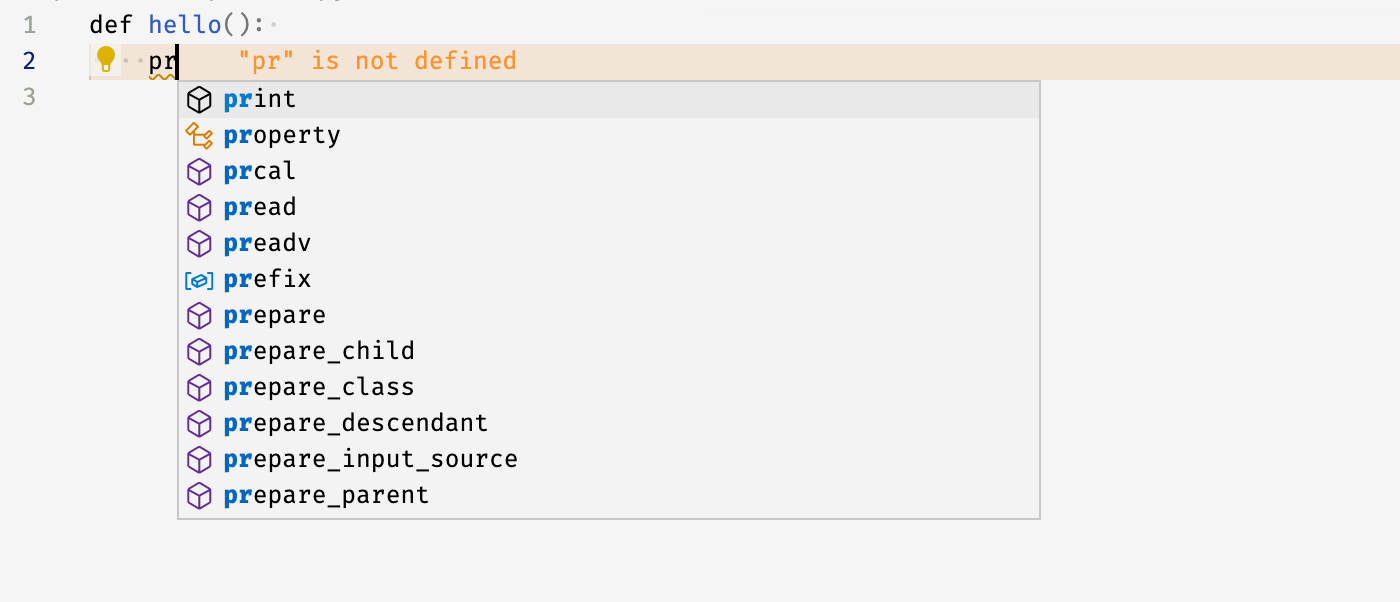
\includegraphics{examples/complete.png}
\caption{Completion options resolved by the Python language server in
Visual Studio Code}\label{fig:lsp-capability-complete}
}
\end{figure}

\hypertarget{sec:hover}{%
\subsubsection{Hover}\label{sec:hover}}

\emph{RPC Method:
\href{https://microsoft.github.io/language-server-protocol/specifications/specification-current/\#textDocument_hover}{\texttt{textDocument/hover}}}

Hover requests are issued by editors when the user rests their mouse
cursor on text in an opened document or issues a designated command in
editors without mouse support. If the language server has indexed any
information corresponding to the position, it can generate a report
using plain text and code elements, which are then rendered by the
editor. Language servers typically use this to communicate
type-signatures or documentation. An example can be seen in
fig.~\ref{fig:lsp-capability-hover}.

\begin{figure}
\hypertarget{fig:lsp-capability-hover}{%
\centering
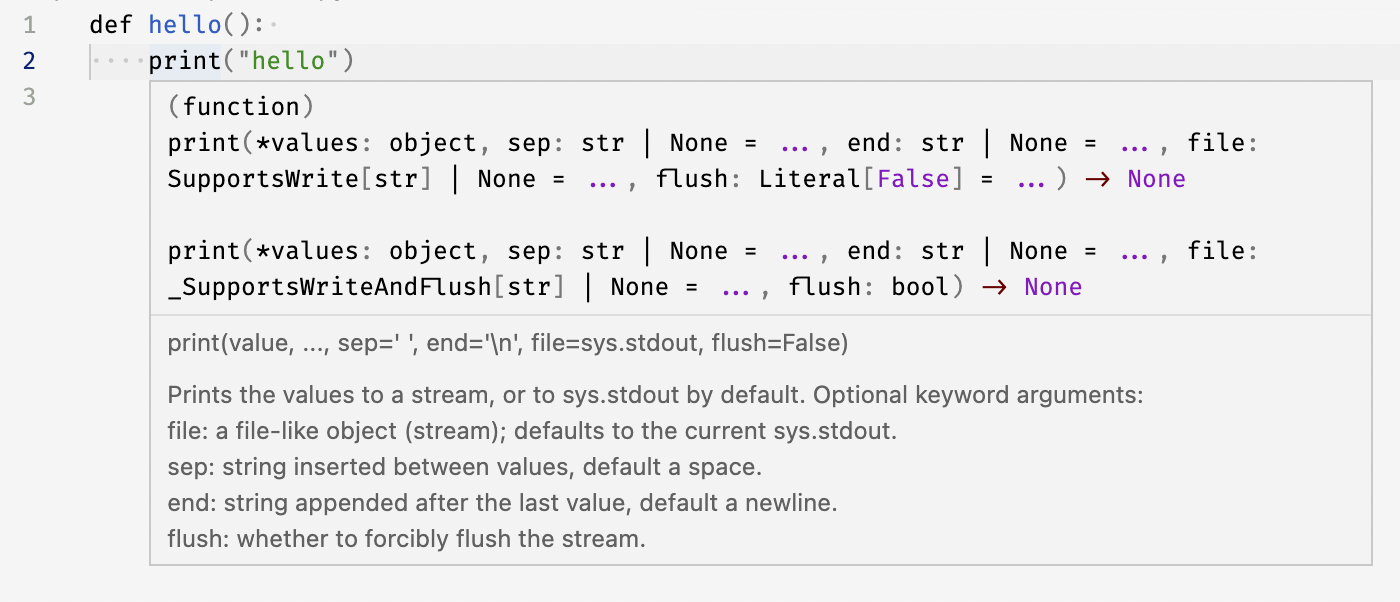
\includegraphics{examples/hover.png}
\caption{Hover information displayed by the Python language server in
Visual Studio Code}\label{fig:lsp-capability-hover}
}
\end{figure}

\hypertarget{sec:jump-to-definition}{%
\subsubsection{Jump to Definition}\label{sec:jump-to-definition}}

\emph{RPC Method:
\href{https://microsoft.github.io/language-server-protocol/specifications/specification-current/\#textDocument_definition}{\texttt{textDocument/definition}}}

The LSP allows users to navigate their code by the means of symbols by
finding the definition of a requested symbol. Symbols can be for
instance variable names or function calls. As seen in
fig.~\ref{fig:lsp-capability-definition}, editors can use the available
information to enrich hover overlays with the hovered element's
definition.

\begin{figure}
\hypertarget{fig:lsp-capability-definition}{%
\centering
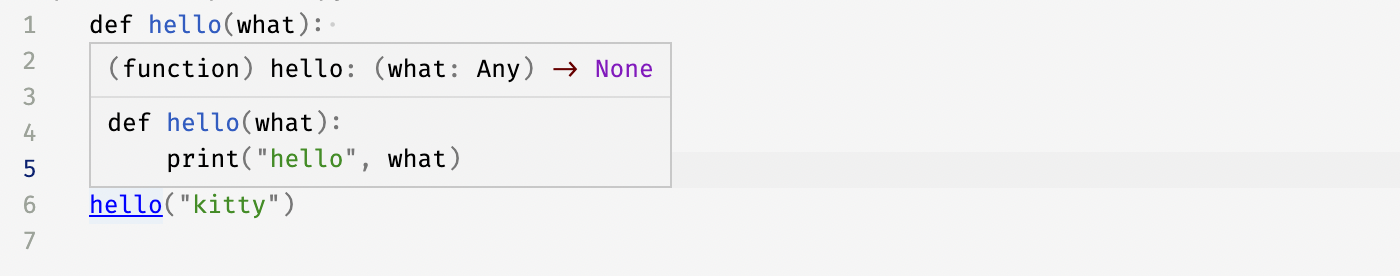
\includegraphics{examples/definition.png}
\caption{Hover information enriched with the definition. Python language
server in Visual Studio Code}\label{fig:lsp-capability-definition}
}
\end{figure}

\hypertarget{sec:find-references}{%
\subsubsection{Find References}\label{sec:find-references}}

\emph{RPC Method:
\href{https://microsoft.github.io/language-server-protocol/specifications/specification-current/\#textDocument_references}{\texttt{textDocument/references}}}

Finding references is the inverse operation to the previously discussed
\emph{Jump to Definition} (cf. \ref{sec:jump-to-definition}). For a
given symbol definition, for example variable, function, function
argument or record field the LSP provides all usages of the symbol
allowing users to inspect or jump to the referencing code position.

\begin{figure}
\hypertarget{fig:lsp-capability-jump-to-definition}{%
\centering
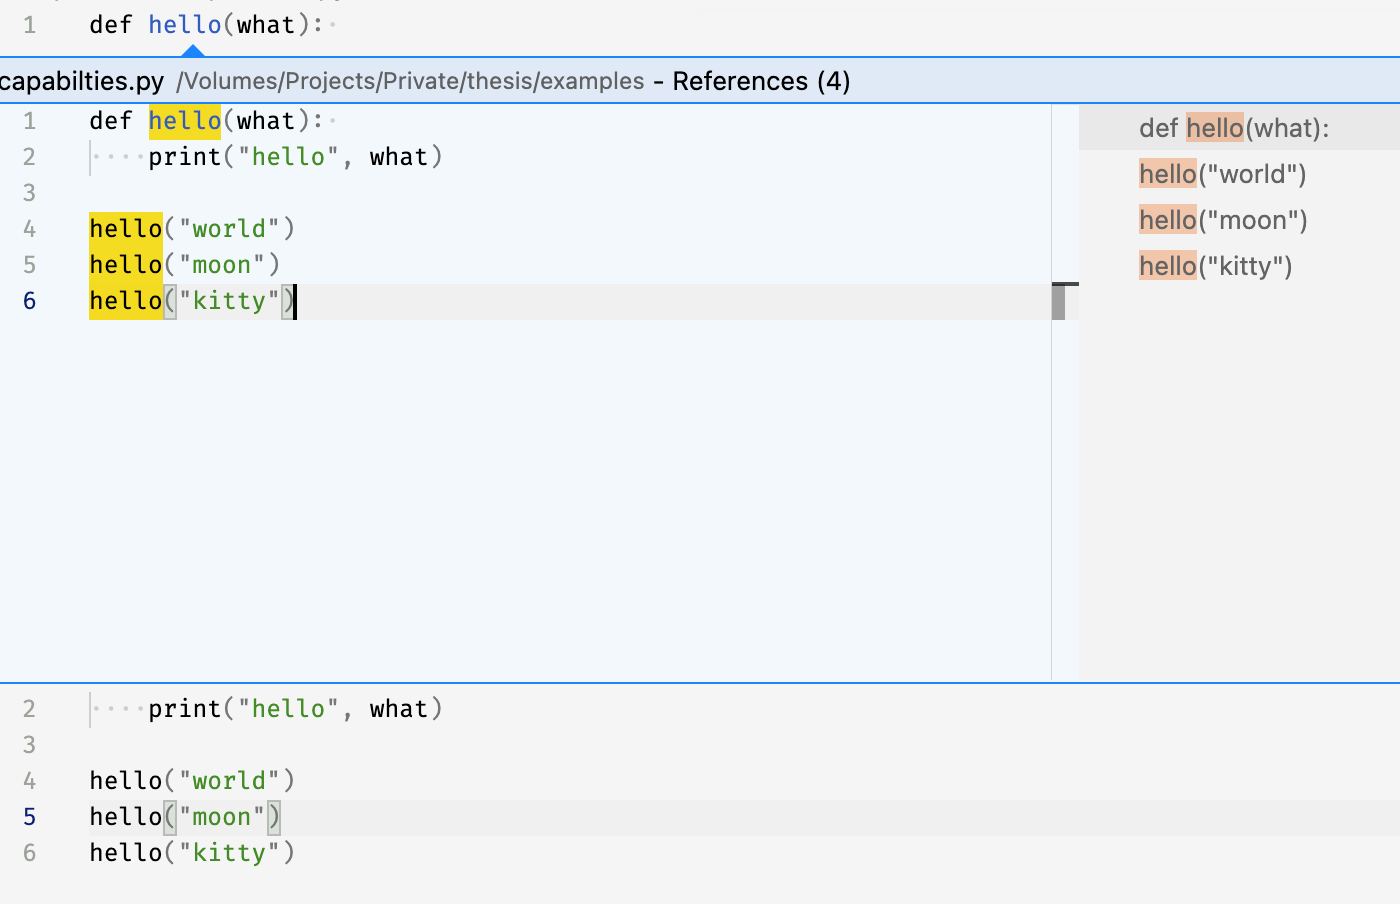
\includegraphics{examples/references.png}
\caption{Listing of all references to the method ``hello.'' Python
language server in Visual Studio
Code}\label{fig:lsp-capability-jump-to-definition}
}
\end{figure}

\hypertarget{sec:workspacedocument-symbols}{%
\subsubsection{Workspace/Document
Symbols}\label{sec:workspacedocument-symbols}}

\emph{RPC Method:
\href{https://microsoft.github.io/language-server-protocol/specifications/lsp/3.17/specification/\#workspace_symbol}{\texttt{textDocument/workspaceSymbol}}
or
\href{https://microsoft.github.io/language-server-protocol/specifications/specification-current/\#textDocument_documentSymbol}{\texttt{textDocument/documentSymbol}}}

The Symbols capability is defined as both a ``Language Feature'' and
``Workspace Feature'' which mainly differ in the scope they represent.
The \texttt{textDocument/documentSymbol} command lists symbols solely
found in the currently opened file, while the \texttt{workspace/symbol}
takes into account all files in the opened set of folders. The
granularity of the listed items is determined by the server and possibly
different for either scope. For instance, document symbols could be as
detailed as listing any kind of method or property found in the
document, while workspace symbols take visibility rules into account
which might expose public entities only. Symbols are associated with a
span of source code of the symbol itself and its context, for example a
function name representing the function body. Moreover, the server can
annotate the items with additional attributes such as symbol kinds, tags
and even child-references (e.g.~for the fields of a record or class).

\hypertarget{sec:diagnostics}{%
\subsubsection{Diagnostics}\label{sec:diagnostics}}

Diagnostics is the collective term for report statements about the
analyzed language of varying severity. This can be parsing or
compilation or type-checking n errors, as well as errors and warnings
issued by a linting tool.

Unlike the preceding features discussed here, diagnostics are a passive
feature, since most often the information stems from external tools
being invoked after source code changes. File updates and diagnostics
are therefore specified as notifications to avoid blocking the
communication.

\hypertarget{sec:file-processing}{%
\subsection{File Processing}\label{sec:file-processing}}

Most language servers handling source code analysis in different ways.
The complexity of the language can be a main influence for the choice of
the approach. Distinctions appear in the way servers process \emph{file
indexes and changes} and how they respond to \emph{requests}.

The LSP supports sending updates in form of diffs of atomic changes and
complete transmission of changed files. The former requires incremental
parsing and analysis, which are challenging to implement but make
processing files much faster upon changes. An incremental approach makes
use of an internal representation of the source code that allows
efficient updates upon small changes to the source file.

Additionally, to facilitate the parsing, an incremental approach must be
able to provide a parser with the right context to correctly parse a
changed fragment of code. In practice, most language servers process
file changes by re-indexing the entire file, discarding the previous
internal state entirely. This is a more approachable method, as it poses
fewer requirements to the architects of the language server. Yet, it is
far less performant. Unlike incremental processing (which updates only
the affected portion of its internal structure), the smallest changes,
including adding or removing lines effect the \emph{reprocessing of the
entire file}. While sufficient for small languages and codebases,
non-incremental processing quickly becomes a performance bottleneck.

For code analysis LSP implementers have to decide between \emph{lazy} or
\emph{greedy} approaches for processing files and answering requests.
Dominantly greedy implementations resolve most available information
during the indexing of the file. The server can then utilize this model
to answer requests using mere lookups. This stands in contrast to lazy
approaches where only minimal local information is resolved during the
indexing. Requests invoke an ad-hoc resolution the results of which may
be memoized for future requests. Lazy resolution is more prevalent in
conjunction with incremental indexing, since it further reduces the work
associated with file changes. This is essential in complex languages
that would otherwise perform a great amount of redundant work.

\hypertarget{sec:text-based-configuration}{%
\section{Text based Configuration}\label{sec:text-based-configuration}}

Configuration languages such as XML{[}13{]}, JSON{[}14{]}, or
YAML{[}15{]} are textual representations of structural data used to
configure parameters of a system or application. The objective of such
languages is to be machine-readable, yet also intuitive enough for
humans to write.

\hypertarget{sec:common-configuration-languages}{%
\subsection{Common Configuration
Languages}\label{sec:common-configuration-languages}}

\hypertarget{sec:json}{%
\subsubsection{JSON}\label{sec:json}}

According to the JSON specification {[}14{]} the language was designed
as a data-interchange format that is easy to read and write both for
humans and machines. Since it is a subset of the JavaScript language,
its use is particularly straight forward and wide spread in JavaScript
based environments such as web applications. But due to its simplicity
implementations are available and for all major languages, motivating
its use for configuration files.

\hypertarget{sec:yaml}{%
\subsubsection{YAML}\label{sec:yaml}}

YAML is another popular language, mainly used for configuration files.
According to its goals it should be human-readable and independent of
the programming language making use of it. It should be efficient to
parse and easy to implement while being expressive and extensible.

YAML also features a very flexible syntax which allows for many
alternative ways to declare semantically equivalent data. For example
boolean expressions can be written as any of the following values:

\begin{quote}
\texttt{y\textbar{}Y\textbar{}yes\textbar{}Yes\textbar{}YES\textbar{}n\textbar{}N\textbar{}no\textbar{}No\textbar{}NO}
\texttt{true\textbar{}True\textbar{}TRUE\textbar{}false\textbar{}False\textbar{}FALSE}
\texttt{on\textbar{}On\textbar{}ON\textbar{}off\textbar{}Off\textbar{}OFF}
\end{quote}

Since YAML facilitates indentation as a way to express objects or lists
and does not require object keys (and even strings) to be quoted, it is
considered easier to write than JSON at the expense of parser
complexity. Yet, YAML is compatible with JSON since as subset of its
specification defines a JSON equivalent syntax that permits the use of
\texttt{\{..\}} and \texttt{{[}..{]}} to describe objects and lists
respectively.

\hypertarget{sec:applications-of-configuration-languages}{%
\subsection{Applications of Configuration
Languages}\label{sec:applications-of-configuration-languages}}

Applications of configuration languages are ubiquitous especially in the
vicinity of software development. While XML and JSON are often used by
package managers {[}18{]}, YAML is a popular choice for complex
configurations such as CI/CD pipelines {[}19{]}--{[}21{]} or machine
configurations in software defined networks such as Kubernetes{[}22{]}
and docker compose {[}23{]}.

Such formats are used due to some significant advantages compared to
other binary formats such as databases. Most strikingly, the textual
representation allows inspection of a configuration without the need of
a separate tool but a text editor. Moreover, textual configuration can
be version controlled using VCS software like Git which allows changes
to be tracked over time. Linux service configurations (files in
\texttt{/etc}) and MacOS \texttt{*.plist} files which can be serialized
as XML or a JSON-like format, especially exemplify that claim.

\hypertarget{sec:configuration-programming-languages}{%
\subsection{Configuration Programming
Languages}\label{sec:configuration-programming-languages}}

Despite the above-mentioned formats being simple to parse and widely
supported {[}14{]}, their static nature rules out any dynamic content
such as generated fields, functions and the possibility to factorize and
reuse. Besides, content validation has to be developed separately, which
led to the design of complementary schema specification languages like
json-schema {[}24{]} or XSD {[}25{]}.

These qualities require an evaluated language. In fact, some
applications make heavy use of config files written in the native
programming language which gives them access to language features and
existing analysis tools. Examples include JavaScript frameworks such as
webpack {[}26{]} or Vue {[}27{]} and python package management using
\texttt{setuptools}{[}28{]}. Yet, the versatility of general purpose
languages poses new security risks if used in this context as
configurations could now contain malicious code requiring additional
verification. Beyond this, not all languages serve as a configuration
language, e.g.~compiled languages.

However, for particularly complex applications, both advanced features
and language independence are desirable. Alternatively to using high
level general purpose languages, this demand is addressed by domain
specific languages (DSL). Dhall {[}29{]}, Cue {[}30{]} or jsonnet
{[}31{]} are such domain specific languages, that offer varying support
for string interpolation, (strict) typing, functions and validation.
Most of these languages are used as a templating system which means a
configuration file in a more portable format is generated using an
evaluation of the more expressive configuration source. The added
expressiveness manifests in the ability to evaluate expression and the
availability of imports, variables and functions. These features allow
refactoring and simplify repetitive configuration files.

\hypertarget{sec:infrastructure-as-code}{%
\subsection{Infrastructure as Code}\label{sec:infrastructure-as-code}}

The shift to an increasing application of IaaS\footnote{Infrastructure
  as a Service} products started the desire for declarative machine
configuration in a bid to simplify the setup and reproducibility of such
systems. This configuration based setup of infrastructure is commonly
summarized as infrastructure as code or IaC. As the name suggests, IaC
puts cloud configuration closer to the domain of software development
{[}32{]}.

In principle, IaaS solutions offer great flexibility with regard to
resource provision (computing, storage, load balancing, etc.), network
setup and scaling of (virtual) servers. However, since the primary
interaction with those systems is imperative and based on command line
or web interfaces, maintaining entire applications' or company's
environments manually comes with obvious drawbacks.

Changing and undoing changes to existing networks requires intricate
knowledge about its topology which in turn has to be meticulously
documented. Undocumented modification pose a significant risk for
\emph{config drift} which is particularly difficult to undo
imperatively. Beyond that, interacting with a system through its
imperative interfaces demands qualified skills of specialized engineers.

The concept of ``Infrastructure as Code'' (\emph{IaC}) align with the
principles of DevOps. IaC tools help to overcome the need for dedicated
teams for \emph{Dev}elopment and \emph{Op}erations by allowing to
declaratively specify the dependencies, topology and virtual resources.
Optimally, different environments for testing, staging and production
can be derived from a common base and changes to configurations are
atomic. As an additional benefit, configuration code is subject to
common software engineering tooling; It can be statically analyzed,
refactored and version controlled to ensure reproducibility. A subset of
IaC is focused on largely declarative configuration based on
configuration files that are interpreted and ``converted'' into
imperative platform dependent instructions.

As a notable instance, the
Nix{[}{[}33{]};dolstraNixSafePolicyFree2004{]} ecosystem even goes as
far as enabling declarative system and service configuration using
NixOps{[}34{]}.

To get an idea of how this would look like, lst.~\ref{lst:nixops-rproxy}
shows the configuration for a deployment of the Git based wiki server
Gollum{[}35{]} behind a nginx reverse proxy on the AWS network. Although
this example targets AWS, Nix itself is platform-agnostic and NixOps
supports different backends through various plugins. Configurations like
this are abstractions over many manual steps and the Nix language
employed in this example allows for even higher level turing-complete
interaction with configurations.

\begin{codelisting}

\caption{Example NixOps deployment to AWS}

\hypertarget{lst:nixops-rproxy}{%
\label{lst:nixops-rproxy}}%
\begin{Shaded}
\begin{Highlighting}[]
\KeywordTok{\{}
  \ExtensionTok{network.description}\NormalTok{ = }\StringTok{"Gollum server and reverse proxy"}\KeywordTok{;}
  \ExtensionTok{defaults}\NormalTok{ = }
    \KeywordTok{\{} \ExtensionTok{config,}\NormalTok{ pkgs, ... \}:}
    \KeywordTok{\{}
      \CommentTok{\# Configuration of a specific deployment implementation}
      \CommentTok{\# here: AWS EC2}
      \ExtensionTok{deployment.targetEnv}\NormalTok{ = }\StringTok{"ec2"}\KeywordTok{;}
      \ExtensionTok{deployment.ec2.accessKeyId}\NormalTok{ = }\StringTok{"AKIA..."}\KeywordTok{;}
      \ExtensionTok{deployment.ec2.keyPair}\NormalTok{ = }\StringTok{"..."}\KeywordTok{;}
      \ExtensionTok{deployment.ec2.privateKey}\NormalTok{ = }\StringTok{"..."}\KeywordTok{;}
      \ExtensionTok{deployment.ec2.securityGroups}\NormalTok{ = pkgs.lib.mkDefault [ }\StringTok{"default"}\NormalTok{ ]}\KeywordTok{;}
      \ExtensionTok{deployment.ec2.region}\NormalTok{ = pkgs.lib.mkDefault }\StringTok{"eu{-}west{-}1"}\KeywordTok{;}
      \ExtensionTok{deployment.ec2.instanceType}\NormalTok{ = pkgs.lib.mkDefault }\StringTok{"t2.large"}\KeywordTok{;}
    \KeywordTok{\};}
  \ExtensionTok{gollum}\NormalTok{ =}
    \KeywordTok{\{} \ExtensionTok{config,}\NormalTok{ pkgs, ... \}:}
    \KeywordTok{\{}
      \CommentTok{\# Nix based setup of the gollum server}
      \ExtensionTok{services.gollum}\NormalTok{ = \{}
        \BuiltInTok{enable}\NormalTok{ = true}\KeywordTok{;}
        \ExtensionTok{port}\NormalTok{ = 40273}\KeywordTok{;}
      \KeywordTok{\};}
      \ExtensionTok{networking.firewall.allowedTCPPorts}\NormalTok{ = [ config.services.gollum.port ]}\KeywordTok{;}
    \KeywordTok{\};}
  \ExtensionTok{reverseproxy}\NormalTok{ =}
    \KeywordTok{\{} \ExtensionTok{config,}\NormalTok{ pkgs, nodes, ... \}:}
    \BuiltInTok{let}
      \ExtensionTok{gollumPort}\NormalTok{ = nodes.gollum.config.services.gollum.port}\KeywordTok{;}
    \ErrorTok{in}
    \KeywordTok{\{}
      \CommentTok{\# Nix based setup of a nginx reverse proxy}
      \ExtensionTok{services.nginx}\NormalTok{ = \{}
        \BuiltInTok{enable}\NormalTok{ = true}\KeywordTok{;}
        \ExtensionTok{virtualHosts.}\StringTok{"wiki.example.net"}\ExtensionTok{.locations.}\StringTok{"/"}\NormalTok{ = \{}
          \ExtensionTok{proxyPass}\NormalTok{ = }\StringTok{"http://gollum:}\VariableTok{$\{toString}\ErrorTok{ gollumPort}\VariableTok{\}}\StringTok{"}\KeywordTok{;}
        \KeywordTok{\};}
      \KeywordTok{\};}
      \ExtensionTok{networking.firewall.allowedTCPPorts}\NormalTok{ = [ 80 ]}\KeywordTok{;}
      \CommentTok{\# Instance can override default deployment options }
      \ExtensionTok{deployment.ec2.instanceType}\NormalTok{ = }\StringTok{"t1.medium"}\KeywordTok{;}
    \KeywordTok{\};}
\KeywordTok{\}}
\end{Highlighting}
\end{Shaded}

\end{codelisting}

Similarly, tools like Terraform{[}36{]}, or Chef{[}37{]} use their own
DSLs and integrate with most major cloud providers. The popularity of
these products\footnote{https://trends.google.com/trends/explore?date=2012-01-01\%202022-01-01\&q=\%2Fg\%2F11g6bg27fp,CloudFormation},
beyond all, highlights the importance of expressive configuration
formats and their industry value.

Finally, descriptive data formats for cloud configurations allow
mitigating security risks through static analysis. Yet, as recently as
Fall 2021 dossiers of Palo Alto Networks' security department Unit 42
{[}38{]} show that a majority of public projects use insecure
configurations. This suggests that techniques{[}39{]} to automatically
check templates are not actively employed, and points out the importance
of evaluated configuration languages which can implement passive
approaches to security analysis.

\hypertarget{sec:nickel}{%
\subsection{Nickel}\label{sec:nickel}}

The Nickel{[}6{]} language is a configuration programming language as
defined in sec.~\ref{sec:configuration-programming-languages} with the
aims of providing composable, verifiable and validatable configuration
files. Nickel implements a pure functional language with JSON-like data
types and turing-complete lambda calculus. The language draws
inspiration from existing projects such as Cue {[}30{]}, Dhall {[}29{]}
and most importantly Nix {[}33{]}. However, Nickel sets itself apart
from the existing projects by combining and advancing their strengths.
The language addresses concerns drawn from the experiences with Nix
which employs a sophisticated module system to provide type-safe,
composed (system) configuration files. Nickel implements gradual type
annotations, with runtime checked contracts to ensure even complex
configurations remain correct. Additionally, considering record merging
on a language level facilitates modularization and composition of
configurations.

\hypertarget{sec:nickel-ast}{%
\subsubsection{Nickel AST}\label{sec:nickel-ast}}

Nickel's syntax tree is a single sum type, i.e., an enumeration of node
types. Each enumeration variant may refer to child nodes, representing a
branch or hold terminal values in which case it is considered a leaf of
the tree. Additionally, tree nodes hold information about their position
in the underlying code.

\hypertarget{sec:basic-elements}{%
\paragraph{Basic Elements}\label{sec:basic-elements}}

The primitive values of the Nickel language are closely related to JSON.
On the leaf level, Nickel defines \texttt{Boolean}, \texttt{Number},
\texttt{String} and \texttt{Null}. In addition to that the language
implements native support for \texttt{Enum} values which are serialized
as plain strings in less expressive formats such as JSON. Each of these
are terminal leafs in the syntax tree.

Completing JSON compatibility, \texttt{List} and \texttt{Record}
constructs are present as well. Records on a syntax level are
Dictionaries, uniquely associating an identifier with a sub-node.

These data types constitute a static subset of Nickel which allows
writing JSON compatible expressions as shown in
lst.~\ref{lst:nickel-static}.

\begin{codelisting}

\caption{Example of a static Nickel expression}

\hypertarget{lst:nickel-static}{%
\label{lst:nickel-static}}%
\begin{verbatim}
{
  list = [ 1, "string", null],
  "some key" = "value"
} 
\end{verbatim}

\end{codelisting}

Beyond these basic elements, Nickel implements variables and functions
as well as a special syntax for attaching metadata and recursive
records.

\hypertarget{sec:identifiers}{%
\paragraph{Identifiers}\label{sec:identifiers}}

The inclusion of variables to the language, implies an understanding of
identifiers. Such name bindings can be declared in multiple ways,
e.g.~\texttt{let} bindings, function arguments and records. The usage of
a name is always parsed as a single \texttt{Var} node wrapping the
identifier. Span information of identifiers is preserved by the parser
and encoded in the \texttt{Ident} type.

\hypertarget{sec:variable-reference}{%
\paragraph{Variable Reference}\label{sec:variable-reference}}

\begin{codelisting}

\caption{Let bindings and functions in nickel}

\hypertarget{lst:nickel-let-binding}{%
\label{lst:nickel-let-binding}}%
\begin{verbatim}
// simple bindings
let name = <expr> in <expr>
let func = fun arg => <expr> in <expr>

// or with patterns
let name @ { field, with_default = 2 } = <expr> in <expr>
let func = fun arg @ { field, with_default = 2 } => 
  <expr> in 
  <expr>
\end{verbatim}

\end{codelisting}

Let bindings in their simplest form merely bind a name to a value
expression and expose the name to the inner expression. Hence, the
\texttt{Let} node contains the binding and links to both implementation
and scope subtrees. The binding can be a simple name, a pattern or both
by naming the pattern as shown in lst.~\ref{lst:nickel-let-binding}.

\begin{codelisting}

\caption{Parsed representation of functions with multiple arguments}

\hypertarget{lst:nickel-args-function}{%
\label{lst:nickel-args-function}}%
\begin{verbatim}
fun first second => first + second
// ...is parsed as
fun first =>
  fun second => first + second
\end{verbatim}

\end{codelisting}

Functions in Nickel are curried lambda expressions. A function with
multiple arguments gets broken down into nested single argument
functions as seen in lst.~\ref{lst:nickel-args-function}. Function
argument name binding therefore looks the same as in \texttt{let}
bindings.

\hypertarget{sec:meta-information}{%
\paragraph{Meta Information}\label{sec:meta-information}}

One key feature of Nickel is its gradual typing system {[}40{]}, which
implies that values can be explicitly typed. Complementing type
information, it is possible to annotate values with contracts and
additional metadata such as contracts, documentation, default values and
merge priority using a special syntax as displayed in
lst.~\ref{lst:nickel-meta}.

\begin{codelisting}

\caption{Example of a static Nickel expression}

\hypertarget{lst:nickel-meta}{%
\label{lst:nickel-meta}}%
\begin{verbatim}
let Contract = { 
  foo | Num 
      | doc "I am foo",
  hello | Str
        | default = "world"
}
| doc "Just an example Contract"
in 
let value | #Contract = { foo = 9, }
in value == { foo = 9, hello = "world", } 

> true
\end{verbatim}

\end{codelisting}

Internally, the addition of annotations wraps the annotated term in a
\texttt{MetaValue}, an additional tree node which describes its subtree.
The expression shown in lst.~\ref{lst:nickel-meta-typed} translates to
the AST in fig.~\ref{fig:nickel-meta-typed}.

\begin{codelisting}

\caption{Example of a typed expression}

\hypertarget{lst:nickel-meta-typed}{%
\label{lst:nickel-meta-typed}}%
\begin{verbatim}
let x: Num = 5 in x
\end{verbatim}

\end{codelisting}

\begin{figure}
\hypertarget{fig:nickel-meta-typed}{%
\centering
\includegraphics[width=\textwidth,height=4.5cm]{graphviz-images/315a516a21d9de4c5e8a5bb47b017725c7516451.pdf}
\caption{AST of typed expression}\label{fig:nickel-meta-typed}
}
\end{figure}

\hypertarget{sec:nested-record-access}{%
\paragraph{Nested Record Access}\label{sec:nested-record-access}}

Nickel supports both static and dynamic access to record fields. If the
field name is statically known, the access is said to be \emph{static}
accordingly. Conversely, if the name requires evaluating a string from
an expression the access is called \emph{dynamic}. An example is given
in lst.~\ref{lst:nickel-static-dynamic}

\begin{codelisting}

\caption{Examples for static and dynamic record access}

\hypertarget{lst:nickel-static-dynamic}{%
\label{lst:nickel-static-dynamic}}%
\begin{verbatim}
let r = { foo = 1, "bar space" = 2} in
r.foo // static
r."bar space" // static
let field = "fo" ++ "o" in r."#{field}" // dynamic
\end{verbatim}

\end{codelisting}

The destruction of record fields is represented using a special set of
AST nodes depending on whether the access is static or dynamic. Static
analysis does not evaluate dynamic fields and thus prevents the analysis
of any deeper element starting with dynamic access. Static access
however can be used to resolve any intermediate reference.

Notably, Nickel represents static access chains in inverse order as
unary operations which in turn puts the terminal \texttt{Var} node as a
leaf in the tree. Figure \ref{fig:nickel-static-access} shows the
representation of the static access performed in
lst.~\ref{lst:nickel-static-access} with the rest of the tree omitted.

\begin{codelisting}

\caption{Nickel static access}

\hypertarget{lst:nickel-static-access}{%
\label{lst:nickel-static-access}}%
\begin{verbatim}
let x = {
  y = {
    z = 1,
  }
} in x.y.z
\end{verbatim}

\end{codelisting}

\begin{figure}
\hypertarget{fig:nickel-static-access}{%
\centering
\includegraphics[width=\textwidth,height=6cm]{graphviz-images/6a93111af06deebabcfa69a99fd1a4c71635ec52.pdf}
\caption{AST of typed expression}\label{fig:nickel-static-access}
}
\end{figure}

\hypertarget{sec:record-shorthand}{%
\paragraph{Record Shorthand}\label{sec:record-shorthand}}

Nickel supports a shorthand syntax to efficiently define nested records
similarly to how nested record fields are accessed. As a comparison the
example in lst.~\ref{lst:nickel-record-shorthand} uses the shorthand
syntax which resolves to the semantically equivalent record defined in
lst.~\ref{lst:nickel-record-no-shorthand}

\begin{codelisting}

\caption{Nickel record defined using shorthand}

\hypertarget{lst:nickel-record-shorthand}{%
\label{lst:nickel-record-shorthand}}%
\begin{verbatim}
{
  deeply.nested.record.field = true,
}
\end{verbatim}

\end{codelisting}

\begin{codelisting}

\caption{Nickel record defined explicitly}

\hypertarget{lst:nickel-record-no-shorthand}{%
\label{lst:nickel-record-no-shorthand}}%
\begin{verbatim}
{
  deeply = {
    nested = {
      record = { 
        field = true,
      }
    }
  }
}
\end{verbatim}

\end{codelisting}

Yet, on a syntax level Nickel generates a different representation.

\hypertarget{sec:record-merging}{%
\subsubsection{Record Merging}\label{sec:record-merging}}

Nickel considers record merging as a fundamental operation that combines
two records (i.e.~JSON objects). Merging is a commutative operation
between two records which takes the fields of both records and returns a
new record that contains the fields of both operands (cf.
lst.~\ref{lst:nickel-merging-simple})

\begin{codelisting}

\caption{Merging of two records without shared fields}

\hypertarget{lst:nickel-merging-simple}{%
\label{lst:nickel-merging-simple}}%
\begin{verbatim}
{ enable = true } & { port = 40273 }
>>
{
  enable = true,
  port = 40273
}
\end{verbatim}

\end{codelisting}

If both operands contain a nested record referred to under the same
name, the merging operation will be applied to these records recursively
(cf. lst.~\ref{lst:nickel-merging-recursive}).

\begin{codelisting}

\caption{Merging of two records without shared nested records}

\hypertarget{lst:nickel-merging-recursive}{%
\label{lst:nickel-merging-recursive}}%
\begin{verbatim}
let enableGollum = {
  service = {
    gollum = {
      enable = true
    }
  } 
} in

let setGollumPort = {
  service = {
    gollum = {
      port = 40273
    }
  } 
} in 

enableGollum & setGollumPort

>> 
{
  service = {
    gollum = {
      enable = true,
      port = 40273
    }
  } 
} 
\end{verbatim}

\end{codelisting}

However, if both operands contain a field with the same name that is not
a mergeable record, the operation fails since both fields have the same
priority making it impossible for Nickel to chose one over the other
(cf. lst.~\ref{lst:nickel-merging-failing-names}) Specifying one of the
fields as a \texttt{default} value allows a single override (cf.
lst.~\ref{lst:nickel-merging-default}). In future versions of Nickel
({[}41{]}) it will be possible to specify priorities in even greater
detail and provide custom merge functions.

\begin{codelisting}

\caption{Failing merge of two records with common field}

\hypertarget{lst:nickel-merging-failing-names}{%
\label{lst:nickel-merging-failing-names}}%
\begin{verbatim}
{ port = 40273 } & { port = 8080 }

>>
error: non mergeable terms
  |
1 | { port = 40273 } & { port = 8080 }
  |          ^^^^^              ^^^^ with this expression
  |          |                   
  |          cannot merge this expression
\end{verbatim}

\end{codelisting}

\begin{codelisting}

\caption{Succeeding merge of two records with default value for common field}

\hypertarget{lst:nickel-merging-default}{%
\label{lst:nickel-merging-default}}%
\begin{verbatim}
{ port | default = 40273 } & { port = 8080 }

>>
{ port = 8080 }
\end{verbatim}

\end{codelisting}

\hypertarget{sec:gradual-typing}{%
\subsubsection{Gradual typing}\label{sec:gradual-typing}}

The typing approach followed by Nickel was introduced by Siek and Taha
{[}40{]} as a combination of static and dynamic typing. The choice
between both type systems is traditionally debated since either approach
imposes specific drawbacks. Static typing lacks the flexibility given by
fully dynamic systems, yet ensures greater correctness by enforcing
value domains. While dynamic typing is often used for prototyping, once
an application or schema stabilizes, the ability to validate data
schemas is usually preferred, often requiring the switch to a different
statically typed language. Gradual typing allows introducing statically
checked types to a program while allowing other parts of the language to
remain untyped and thus interpreted dynamically.

\hypertarget{sec:contracts}{%
\subsubsection{Contracts}\label{sec:contracts}}

In addition to a static type-system Nickel integrates a contract system
akin what is described in {[}42{]}. First introduced by Findler and
Felleisen, contracts allow the creation of runtime-checked subtypes.
Unlike types, contracts check an annotated value using arbitrary
functions that either pass or \emph{blame} the input. Contracts act like
assertions that are automatically checked when a value is used or passed
to annotated functions.

For instance, a contract could be used to define TCP port numbers, like
shown in lst.~\ref{lst:nickel-sample-contract}.

\begin{codelisting}

\caption{Sample Contract ensuring that a value is a valid TCP port number}

\hypertarget{lst:nickel-sample-contract}{%
\label{lst:nickel-sample-contract}}%
\begin{verbatim}
let Port | doc "A contract for a port number" =
  contracts.from_predicate (
    fun value =>
      builtins.is_num value &&
      value % 1 == 0 &&
      value >= 0 &&
      value <= 65535
  )
in 8080 | #Port
\end{verbatim}

\end{codelisting}

Going along gradual typing, contracts pose a convenient alternative to
the \texttt{newtype} pattern. Instead of requiring values to be wrapped
or converted into custom types, contracts are self-contained. As a
further advantage, multiple contracts can be applied to the same value
as well as integrated into other higher level contracts. An example can
be observed in lst.~\ref{lst:nickel-sample-advanced-contract}

\begin{codelisting}

\caption{More advaced use of contracts restricting values to an even smaller domain}

\hypertarget{lst:nickel-sample-advanced-contract}{%
\label{lst:nickel-sample-advanced-contract}}%
\begin{verbatim}
let Port | doc "A contract for a port number" =
  contracts.from_predicate (
    fun value =>
      builtins.is_num value &&
      value % 1 == 0 &&
      value >= 0 &&
      value <= 65535
  )
in
let UnprivilegedPort = contracts.from_predicate (
  fun value =>
    (value | #Port) >= 1024  
  )
in
let Even = fun label value =>
  if value % 2 == 0 then value
  else
    let msg = "not an even value" in
    contracts.blame_with msg label
in

8001 | #UnprivilegedPort
     | #Even
\end{verbatim}

\end{codelisting}

Notice how contracts also enable detailed error messages (see
lst.~\ref{lst:nickel-sample-error-advaced-contract}) using custom blame
messages. Nickel is able to point to the exact value violating a
contract as well as the contract in question.

\begin{codelisting}

\caption{Example error message for failed contract}

\hypertarget{lst:nickel-sample-error-advaced-contract}{%
\label{lst:nickel-sample-error-advaced-contract}}%
\begin{verbatim}
error: Blame error: contract broken by a value [not an even value].
    - :1:1
   |
 1 | #Even
   | ----- expected type
   |
    - repl-input-34:22:1
   |  
22 | - 8001 | #UnprivilegedPort
   |   ---- evaluated to this expression
23 | |      | #Even
   | -------------^ applied to this expression

note: 
    - repl-input-34:23:8
   |
23 |      | #Even
   |        ^^^^^ bound here
\end{verbatim}

\end{codelisting}

\hypertarget{sec:related-work}{%
\chapter{Related work}\label{sec:related-work}}

The Nickel Language Server follows a history of previous research and
development in the domain of modern language tooling and editor
integration. Most importantly, it is part of a growing set of LSP
integrations. As such, it is important to get a picture of the field of
current LSP projects and the approaches leading up to the LSP. This
chapter will first introduce and show the shortcomings of classical IDE
based language tooling as well as early advances towards editor
independent implementations. The following section displays particular
instances of different approaches towards the implementation of language
servers. Projects that extend and supplement or take inspiration from
the LSP, are portrayed in the final section.

\hypertarget{sec:ide-support}{%
\section{IDE Support}\label{sec:ide-support}}

\hypertarget{sec:native-and-plugin-systems}{%
\subsection{Native and Plugin
Systems}\label{sec:native-and-plugin-systems}}

Before the invention of the Language Server Protocol, language
intelligence used to be provided by an IDE. Yet, the range of officially
supported languages remained relatively small\footnote{https://www.jetbrains.com/products/}.
While integration for popular languages was common, top-tier support for
less popular ones was all but guaranteed and relied mainly on community
efforts. In fact Eclipse{[}44{]}, IntelliJ{[}45{]}, and Visual
Studio{[}46{]}, to this day the most popular IDE choices, focus on a
narrow subset of languages, historically Java and .NET. Additional
languages can be integrated by custom (third-party) plugins or
derivatives of the base platform. Due to the technical implications,
plugins are generally not compatible between different platforms. Many
less popular languages therefore saw redundant implementations of what
is essentially the same. For Haskell separate efforts produced an
eclipse based IDE{[}47{]}, as well as independent IntelliJ
plugins{[}49{]}. Importantly, the implementers of the former reported
troubles with the language barrier between Haskell and the Eclipse base
written in Java.

The Haskell language is an exceptional example since there is also a
native Haskell IDE{[}50{]} albeit that it is available only to the MacOS
operating system. This showcases the difficulties of language tooling
and its provision, since all of these projects are platform dependent
and differ in functionality. Moreover, effectively the same tool is
developed multiple times wasting resources.

In general, developing language integrations, both as the vendor of an
IDE or a third-party plugin developer requires extensive resources.
Table \ref{tbl:plugins-size} gives an idea of the efforts required.
Since the IntelliJ platform is based on the JVM, its plugin system
requires the use of JVM languages{[}51{]}, making it hard to reuse the
code of e.g.~a reference compiler or interpreter. The Rust and Haskell
integrations for instance contain at best only a fraction of code in
their respective language.

\hypertarget{tbl:plugins-size}{}
\begin{longtable}[]{@{}
  >{\raggedright\arraybackslash}p{(\columnwidth - 2\tabcolsep) * \real{0.29}}
  >{\raggedright\arraybackslash}p{(\columnwidth - 2\tabcolsep) * \real{0.71}}@{}}
\caption{\label{tbl:plugins-size}Comparison of the size for different
IntelliJ platform plugins}\tabularnewline
\toprule
\begin{minipage}[b]{\linewidth}\raggedright
Plugin
\end{minipage} & \begin{minipage}[b]{\linewidth}\raggedright
lines of code
\end{minipage} \\
\midrule
\endfirsthead
\toprule
\begin{minipage}[b]{\linewidth}\raggedright
Plugin
\end{minipage} & \begin{minipage}[b]{\linewidth}\raggedright
lines of code
\end{minipage} \\
\midrule
\endhead
intellij-haskell & 17249 (Java) + 13476 (Scala) \textbf{+ 0
(Haskell)} \\
intellij-rust & 229131 (Kotlin) + 3958 (Rust) \\
intellij-scala & 39382 (Java) + 478904 (Scala) \\
intellij-kotlin & 182372 (Java) + 563394 (Kotlin) \\
intellij-community/python & 47720 (C) + 248177 (Java) + 37101 (Kotlin) +
277125 (Python) \\
\bottomrule
\end{longtable}

Naturally, development efforts at this size tend to gravitate around the
most promising solution, stifling the progress on competing platforms.
Editor-specific approaches also tend to lock-in programmers into a
specific platform for its language support regardless of their personal
preference.

\hypertarget{sec:server-client-abstractions}{%
\subsection{Server Client
Abstractions}\label{sec:server-client-abstractions}}

\hypertarget{sec:monto}{%
\subsubsection{Monto}\label{sec:monto}}

The authors of the Monto project{[}2{]} call this the ``IDE Portability
Problem.'' They compare the situation with the task of compiling
different high level languages to a set of CPU architectures. In
Compilers, the answer to that problem was the use of an intermediate
representation (IR). A major compiler toolchain making use of this is
the LLVM{[}53{]}. Compiler frontends for different languages --
e.g.~Clang{[}54{]}, Rustc{[}55{]}, NVCC{[}56{]},\ldots{} -- compile
input languages into LLVM IR, a low level language with additional
capabilities to provide optimization hints but independent of a
particular architecture. LLVM performs optimization of the IR and passes
it to a compiler backend which in turn generates bytecode for specific
architectures e.g.~\texttt{x86\_64}, \texttt{MIPS}, \texttt{aarch64},
\texttt{wasm}, etc. Notably through this mechanism, languages gain
support for a range of architectures and profit from existing
optimizations developed for the IR.

With Monto, Kreidel et al propose a similar idea for IDE portability.
The paper describes the \emph{Monto IR} and how they use a \emph{Message
Broker} to receive events from the Editor and dispatch them to
\emph{Monto Services}.

The Monto IR is a language-agnostic and editor-independent tree-like
model serialized as JSON. Additionally, the IR maintains low level
syntax highlighting information (font, color, style, etc.) but leaves
the highlighting to the language specific service.

The processing and modification of the source code and IR is performed
by \emph{Monto Services}. Services implement specific actions,
e.g.~parsing, outlining or highlighting. A central broker connects the
services with each other and the editor.

Since Monto performs all work on the IR, independent of the editor, and
serializes the IR as JSON messages, the language used to implement
\emph{Monto Services} can be chosen freely giving even more flexibility.

The Editor extension's responsibility is to act as a source and sink for
data. It sends Monto compliant messages to the broker and receives
processing results such as (error) reports. The communication is based
on the ZeroMQ{[}57{]} technology which was chosen because it is
lightweight and available in manly languages{[}2{]} allowing to make use
of existing language tools.

\hypertarget{sec:merlin}{%
\subsubsection{Merlin}\label{sec:merlin}}

The Merlin tool{[}1{]} is in many ways a more specific version of the
idea presented in Monto. Merlin is a language server for the Ocaml
language, yet predates the Language Server Protocol.

The authors of Merlin postulate that implementing ``tooling support
traditionally provided by IDEs'' for ``niche languages'' demands to
``share the language-awareness logic'' between implementations. As an
answer to that, they describe the architecture of Merlin in {[}1{]}.

Similarly to Monto, Merlin separates editor extensions from language
analysis. However, Merlin uses a command line interface instead of
message passing for interaction. Editor extensions expose the server
functions to the user by integrating with the editor.

Thanks to this architecture, the Merlin developers have been able to
focus their efforts on a single project providing intelligence for OCaml
source code. The result of this work is a platform independent,
performant and fault-tolerant provider of language intelligence. Low
level changes to the compiler core have been made to provide incremental
parsing, type-checking and analysis. Apart from more efficient handling
of source changes, this allows users to query information even about
incomplete or incorrect programs.

Since both Merlin and the OCaml compiler are written in OCaml, Merlin is
able to reuse large parts of the reference OCaml implementation. This
allows Merlin to avoid reimplementing every single feature of the
language. Still, incremental parsing and typechecking is not a priority
to the compiler which prompted the developers of Merlin to vendor
modified versions of the core OCaml components.

While Merlin serves as a single implementation used by all clients,
unlike Monto it does not specify a language independent format, or
service architecture. In fact, Merlin explicitly specializes in a single
language and provides a complete implementation where Monto merely
defines the language agnostic interface to implement a server on.

\hypertarget{sec:language-servers}{%
\section{Language Servers}\label{sec:language-servers}}

The LSP project was announced{[}60{]} in 2016 to establish a common
protocol over which language tooling could communicate with editors. The
LSP helps the language intelligence tooling to fully concentrate on
source analysis instead of integration with specific editors by building
custom GUI elements and being restricted to editors extension interface.

At the time of writing the LSP is available in version `3.16{[}12{]}.
Microsoft's official website lists 172 implementations of the LSP{[}4{]}
for an equally impressive number of languages.

An in-depth survey of these is outside the scope of this work. Yet, a
few implementations stand out due to their sophisticate architecture,
features, popularity or closeness to the presented work.

Since the number of implementations of the LSP is continuously growing,
this thesis will present a selected set of notable projects. The
presented projects exemplify different approaches with respect to
reusing and interacting with the existing language implementation of the
targeted language. In particular, the following five approaches are
discussed:

\begin{enumerate}
\def\labelenumi{\arabic{enumi}.}
\tightlist
\item
  Three complete implementations that tightly integrate with the
  implementation level tooling of the respective language:
  \emph{rust-analyzer{[}61{]}, }ocaml-lsp\emph{/}merlin{[}1{]} and the
  *Haskell Language Server{[}62{]}
\item
  A project that indirectly interacts with the language implementation
  through an interactive programming shell (REPL). \emph{Frege
  LSP{[}64{]}}
\item
  A Language Server that is completely independent of the target
  language's runtime. Highlighting how basic LSP support can be
  implemented even for small languages in terms of userbase and
  complexity. *rnix-lsp{[}66{]}
\item
  Two projects that facilitate the LSP as an interface to an existing
  tool via HTTP or command line. \emph{CPAchecker{[}68{]} and
  }CodeCompass{[}69{]}
\item
  An approach to generate language servers from domain specific language
  specifications{[}70{]}.
\end{enumerate}

\hypertarget{sec:integrating-with-the-compilerruntime}{%
\subsection{Integrating with the
Compiler/Runtime}\label{sec:integrating-with-the-compilerruntime}}

Today LSP-based solutions serve as the go-to method to implement
language analysis tools. Emerging languages in particular take advantage
from the flexibility and reach of the LSP. Especially the freedom of
choice for the implementing language, is facilitated by multiple
languages by integrating modules of the original compiler or runtime
into the language server.

\hypertarget{sec:hls}{%
\subsubsection{HLS}\label{sec:hls}}

For instance the Haskell language server facilitates a plugin system
that allows it to integrate with existing tooling projects\footnote{https://hackage.haskell.org/packages/browse?terms=hls}.
Plugins provide capabilities for linting, formatting, documentation and
other code actions across multiple compiler versions. This architecture
allows writing an LSP in a modular fashion in the targeted language at
the expense of requiring HSL to use the same compiler version in use by
the IDE and its plugins. This is to ensure API compatibility between
plugins and the compiler.

\hypertarget{sec:ocaml-lsp}{%
\subsubsection{Ocaml LSP}\label{sec:ocaml-lsp}}

Similarly, the Ocaml language service builds on top of existing
infrastructure by relying on the Merlin project introduced in
sec.~\ref{sec:merlin}. Here, the advantages of employing existing
language components have been explored even before the LSP.

\hypertarget{sec:rust-analyzer}{%
\subsubsection{Rust-Analyzer}\label{sec:rust-analyzer}}

The rust-analyzer{[}61{]} takes an intermediate approach. It does not
reuse or modify the existing compiler, but instead implements analysis
functionality based on low level components. This way the developers of
rust-analyzer have greater freedom to adapt for more advanced features.
For instance rust-analyzer implements an analysis optimized parser with
support for incremental processing. Due to the complexity of the
language, LSP requests are processed lazily, with support for caching to
ensure performance. While many parts of the language have been
reimplemented with a language-server-context in mind, the analyzer did
not however implement detailed linting or the rust-specific borrow
checker. For these kinds of analysis, rust-analyzer falls back to calls
to the rust build system.

\hypertarget{sec:frege-lsp}{%
\subsubsection{Frege LSP}\label{sec:frege-lsp}}

While the previous projects integrated into the compiler pipeline and
processed the results separately, other approaches explored the
possiblity to shift the entire analysis to existing modules. A good
example for this method is given by the Frege language\footnote{https://github.com/Frege/frege}.

Frege as introduced in{[}63{]} is a JVM based functional language with a
Haskell-like syntax. It features lazy evaluation, user-definable
operators, type classes and integration with Java.\\
While previously providing an eclipse plugin\footnote{https://github.com/Frege/eclipse-plugin},
the tooling efforts have since been put towards an LSP implementation.
The initial development of this language server has been reported on
in{[}64{]}. The author shows though multiple increments how they
utilized the JVM to implement a language server in Java for the (JVM
based) Frege language. In the final proof-of-concept, the authors build
a minimal language server through the use of Frege's existing REPL and
interpreter modules. The file loaded into the REPL environment providing
basic syntax and type error reporting. The Frege LSP then translates LSP
requests into expressions, evaluates them in the REPL environment and
wraps the result in a formal LSP response. Being written in Java, allows
the server to make use of other community efforts such as the LSP4J
project which provide abstractions over the interaction with LSP
clients. Through the use of abstraction like the Frege REPL, servers can
focus on the implementation of capabilities only, albeit with the limits
set by the interactive environment.

\hypertarget{sec:runtime-independent-lsp-implementations}{%
\subsubsection{Runtime-independent LSP
implementations}\label{sec:runtime-independent-lsp-implementations}}

While many projects do so, language servers do not need to reuse any
existing infrastructure of a targeted language at all. Often, language
implementations do not expose the required language interfaces (parsing,
AST, Types, etc..), or pose various other impediments such as a closed
source, licensing, or the absence of LSP abstractions available for the
host language.

An instance of this type is the rnix-lsp{[}66{]} language server for the
Nix{[}65{]} programming language. Despite the Nix language being written
in C++{[}33{]}, its language server builds on a custom parser called
``rnix{[}71{]} in Rust. However, since rnix does not implement an
interpreter for nix expressions the rnix based language server is
limited to syntactic analysis and changes.

\hypertarget{sec:language-server-as-an-interface-to-cli-tools}{%
\subsubsection{Language Server as an Interface to CLI
tools}\label{sec:language-server-as-an-interface-to-cli-tools}}

While language servers are commonly used to provide code based analytics
and actions such as refactoring, it also proved suitable as a general
interface for existing external tools. These programs may provide common
LSP features or be used to extend past the LSP.

\hypertarget{sec:cpachecker}{%
\paragraph{CPAchecker}\label{sec:cpachecker}}

The work presented by Leimeister in{[}68{]} exemplifies how LSP
functionality can be provided by external tools. The server can be used
to automatically perform software verification in the background using
CPAchecker{[}67{]}. CPAchecker is a platform for automatic and
extensible software verification. The program is written in Java and
provides a command line interface to be run locally. Additionally, it is
possible to execute resource intensive verification through an HTTP-API
on more powerful machines or clusters{[}73{]}. The LSP server supports
both modes of operation. While it can interface directly with the Java
modules provided by the CPAchecker library, it is also able to utilize
an HTTP-API provided by a server instance of the verifier.

\hypertarget{sec:codecompass}{%
\paragraph{CodeCompass}\label{sec:codecompass}}

Similar to the work by Leimeister (c.f sec.~\ref{sec:cpachecker}), in
{[}74{]} Mészáros et al.~present a proof of concept leveraging the LSP
to integrate (stand-alone) code comprehension tools with the LSP
compliant VSCode editor. Code comprehension tools support the work with
complex code bases by ``providing various textual information,
visualization views and source code metrics on multiple abstraction
levels.'' Pushing the boundaries of LSP use-cases, code comprehension
tools do not only analyze specific source code, but also take into
account contextual information. One of such tools is
CodeCompass{[}69{]}. The works of Mészáros yielded a language server
that allowed to access the analysis features of CodeCompass in VSCode.
In their paper they specifically describe the generation of source code
diagrams. Commands issued by the client are processed by a CodeCompass
plugin which acts as an LSP server and interacts with CodeCompass
through internal APIs.

\hypertarget{sec:language-servers-generation-for-domain-specific-languages}{%
\subsection{Language Servers generation for Domain Specific
Languages}\label{sec:language-servers-generation-for-domain-specific-languages}}

Bünder and Kuchen{[}70{]} highlight the importance of the LSP in the
area of Domain Specific Languages (DSL). Compared to general purpose
languages, DSLs often targets both technical and non-technical users.
While DSL creation workbenches like Xtext{[}75{]}, Spoofax{[}76{]} or
MPS{[}77{]} allow for the implementation and provision of Eclipse or
IntelliJ based DSLs, tooling for these languages is usually tied to the
underlying platform. Requiring a specific development platform does not
satisfy every user of the language. Developers have their editor of
choice, that they don't easily give up on. Non-technical users could
easily be overwhelmed by a complex software like Eclipse. For those
non-technical users, a light editor would be more adapted, or even one
that is directly integrated into their business application. The authors
of{[}70{]} present how Xtext can generate an LSP server for a custom
DSL, providing multi-editor support. The authors especially mention the
Monaco Editor{[}78{]}, a reusable HTML component for code editing using
web technologies. It is used in products like VSCode, Theia{[}79{]} and
other web accessible code editors. The Monaco Editor supports the LSP as
a client (that is, on the editor side). Such LSP-capable web editors
make integrating DSLs directly into web applications easier than ever
before.

\hypertarget{sec:alternative-approaches}{%
\section{Alternative approaches}\label{sec:alternative-approaches}}

\hypertarget{sec:lsp-extensions}{%
\subsection{LSP Extensions}\label{sec:lsp-extensions}}

The LSP defines a large range of commands and capabilities which is
continuously being extended by the maintainers of the protocol. Yet,
occasionally server developers find themselves in need of functionality
not yet present in the protocol. For example the LSP does not provide
commands to exchange binary data such as files. In
sec.~\ref{sec:runtime-independent-lsp-implementations} the CodeCompass
Language Server was introduced. A stern feature of this server is the
ability to generate and show diagrams in SVG format. However, the LSP
does not define the concept of \emph{requesting diagrams}. In particular
Mészáros et al.~describe different shortcomings of the LSP :

\begin{enumerate}
\def\labelenumi{\arabic{enumi}.}
\item
  \begin{quote}
  ``LSP doesn't have a feature to place a context menu at an arbitrary
  spot in the document''
  \end{quote}

  Context menu entries are implemented by clients based on the agreed
  upon capabilities of the server. Undefined capabilities cannot be
  added to the context menu.

  In the case of CodeCompass the developers made up for this by using
  the code completion feature as an alternative dynamic context menu.
\item
  \begin{quote}
  ``LSP does not support displaying pictures (diagrams).''
  \end{quote}

  CodeCompass generates diagrams for selected code. Yet, there is no
  image transfer included with the LSP. Since the LSP is based on
  JSON-RPC messages, the authors' solution was to define a new command,
  specifically designed to tackle this non-standard use case.
\end{enumerate}

Missing features of the protocol such as the ones pointed out by
Mészáros et al.~appear frequently, especially in complex language
servers or ones that implement more than basic code processing.

The rust-analyzer defines almost thirty non-standard
commands\footnote{https://rust-analyzer.github.io/manual.html\#features},
to enable different language specific actions.

Taking the idea of the CodeCompass project further, Rodriguez-Echeverria
et al.~propose a generic extension of the LSP for graphical
modeling{[}80{]}. Their approach is based on a generic intermediate
representation of graphs which can be generated by language servers and
turned into a graphical representation by the client implementation.

Similarly, in {[}81{]}, {[}82{]} the authors describe a method to
develop language agnostic LSP extensions. In their work they defined a
language server protocol for specification languages (SLSP) which builds
on top of the existing LSP. The SLSP defines several extensions that
each group the functionality of specific domains. However, unlike other
LSP extensions that are added to facilitate functions of a specific
server, SLSP is language agnostic. In effect, the protocol extensions
presented by Rask et. al.~are reusable across different specification
languages, allowing clients to implements a single frontend. Given their
successes with the presented work, the authors encourage to build
abstract, sharable extensions over language specific ones if possible.

\hypertarget{sec:language-server-index-format}{%
\subsection{Language Server Index
Format}\label{sec:language-server-index-format}}

Nowadays, code hosting platforms are an integral part of the developer
tool set (GitHub, Sourcegraph, GitLab, Sourceforge, etc.). Those
platforms commonly display code simply as text, highlighted at best.
LSP-like features would make for a great improvement for code navigation
and code reading online. Yet, building these features on language
servers would incur redundant and wasteful as a server needed to be
started each time a visitor loads a chunk of code. Since the hosted code
is most often static and precisely versioned, code analysis could be
performed ahead of time, for all files of each version. The LSIF
(Language Server index Format) specifies a schema for the output of such
ahead of time code analysis. Clients can then provide efficient code
intelligence using the pre-computed and standardized index.

The LSIF format encodes a graphical structure which mimics LSP types.
Vertices represent higher level concepts such as \texttt{document}s,
\texttt{range}s, \texttt{resultSet}s and actual results. The relations
between vertices are expressed through the edges.

For instance, hover information as introduced in sec.~\ref{sec:hover}
for the interface declaration in lst.~\ref{lst:lsif-code-sample} can be
represented using the LSIF. Figure \ref{fig:lsif-example} visualizes the
result (cf. lst.~\ref{lst:lsif-result-sample}). Using this graph an LSIF
tool is able to resolve statically determined hover information by
performing the following steps.

\begin{enumerate}
\def\labelenumi{\arabic{enumi}.}
\tightlist
\item
  Search for \texttt{textDocument/hover} edges.
\item
  Select the edge that originates at a \texttt{range} vertex
  corresponding to the requested position.
\item
  Return the target vertex.
\end{enumerate}

\begin{codelisting}

\caption{Exemplary code snippet to showing LSIF formatting}

\hypertarget{lst:lsif-code-sample}{%
\label{lst:lsif-code-sample}}%
\begin{Shaded}
\begin{Highlighting}[]
\NormalTok{export interface ResultSet \{}
\NormalTok{\}}
\end{Highlighting}
\end{Shaded}

\end{codelisting}

\begin{figure}
\hypertarget{fig:lsif-example}{%
\centering
\includegraphics{plantuml-images/2dba35d56975f763ebad1e994af228d0b99b901c}
\caption{LSIF encoded graph for the exemplary code}\label{fig:lsif-example}
}
\end{figure}

\begin{codelisting}

\caption{LSIF formated analysis result}

\hypertarget{lst:lsif-result-sample}{%
\label{lst:lsif-result-sample}}%
\begin{Shaded}
\begin{Highlighting}[]
\NormalTok{\{ }\BuiltInTok{id}\NormalTok{: }\DecValTok{1}\NormalTok{, }\BuiltInTok{type}\NormalTok{: }\StringTok{"vertex"}\NormalTok{, label: }\StringTok{"document"}\NormalTok{, uri: }\StringTok{"file:///..."}\NormalTok{, languageId: }\StringTok{"typescript"}\NormalTok{ \}}
\NormalTok{\{ }\BuiltInTok{id}\NormalTok{: }\DecValTok{2}\NormalTok{, }\BuiltInTok{type}\NormalTok{: }\StringTok{"vertex"}\NormalTok{, label: }\StringTok{"resultSet"}\NormalTok{ \}}
\NormalTok{\{ }
   \BuiltInTok{id}\NormalTok{: }\DecValTok{3}\NormalTok{, }
  \BuiltInTok{type}\NormalTok{: }\StringTok{"vertex"}\NormalTok{, }
\NormalTok{  label: }\StringTok{"range"}\NormalTok{,}
\NormalTok{  start: \{ line: }\DecValTok{0}\NormalTok{, character: }\DecValTok{9}\NormalTok{\}, }
\NormalTok{  end: \{ line: }\DecValTok{0}\NormalTok{, character: }\DecValTok{12}\NormalTok{ \} }
\NormalTok{\}}
\NormalTok{\{ }\BuiltInTok{id}\NormalTok{: }\DecValTok{4}\NormalTok{, }\BuiltInTok{type}\NormalTok{: }\StringTok{"edge"}\NormalTok{, label: }\StringTok{"contains"}\NormalTok{, outV: }\DecValTok{1}\NormalTok{, inVs: [}\DecValTok{3}\NormalTok{] \}}
\NormalTok{\{ }\BuiltInTok{id}\NormalTok{: }\DecValTok{5}\NormalTok{, }\BuiltInTok{type}\NormalTok{: }\StringTok{"edge"}\NormalTok{, label: }\StringTok{"next"}\NormalTok{, outV: }\DecValTok{3}\NormalTok{, inV: }\DecValTok{2}\NormalTok{ \}}
\NormalTok{\{ }
  \BuiltInTok{id}\NormalTok{: }\DecValTok{6}\NormalTok{, }
  \BuiltInTok{type}\NormalTok{: }\StringTok{"vertex"}\NormalTok{,}
\NormalTok{  label: }\StringTok{"hoverResult"}\NormalTok{,}
\NormalTok{  result: \{}
    \StringTok{"contents"}\NormalTok{:[}
\NormalTok{      \{}\StringTok{"language"}\NormalTok{:}\StringTok{"typescript"}\NormalTok{,}\StringTok{"value"}\NormalTok{:}\StringTok{"function bar(): void"}\NormalTok{\},}
      \StringTok{""}
\NormalTok{    ]}
\NormalTok{  \}}
\NormalTok{\}}
\NormalTok{\{ }\BuiltInTok{id}\NormalTok{: }\DecValTok{7}\NormalTok{, }\BuiltInTok{type}\NormalTok{: }\StringTok{"edge"}\NormalTok{, label: }\StringTok{"textDocument/hover"}\NormalTok{, outV: }\DecValTok{2}\NormalTok{, inV: }\DecValTok{6}\NormalTok{ \}}
\end{Highlighting}
\end{Shaded}

\end{codelisting}

An LSIF report is a mere list of \texttt{edge} and \texttt{vertex}
nodes, which allows it to easily extend and connect more subgraphs,
corresponding to more elements and analytics. As a consequence, a subset
of LSP capabilities can be provided statically based on the preprocessed
LSIF model.

\hypertarget{sec:abstracting-software-development-processes}{%
\subsection{Abstracting software development
processes}\label{sec:abstracting-software-development-processes}}

Since its introduction the Language Server Protocol has become a
standard format to provide language tooling for editing source code.
Meanwhile, as hinted in sec.~\ref{sec:lsp-extensions}, the LSP is not
able to fully satisfy every use-case sparking the development of various
LSP extensions. Following the success of language servers, similar
advances have been made in other parts of the software development
process.

For instance, many Java build tools expose software build abstractions
through the Build Server Protocol{[}83{]}, allowing IDEs to integrate
more languages more easily by leveraging the same principle as the LSP.
The BSP provides abstractions over dependencies, build targets,
compilation and running of projects. While the LSP provides \texttt{run}
or \texttt{test} integration for selected languages through Code Lenses,
this is not part of the intended responsibilities of the protocol. In
contrast, those tasks are explicitly targeted by the BSP.

Next to \emph{writing} software (LSP) and
\emph{building/running/testing} software (e.g.~BSP), \emph{debugging}
presents a third principal task of software development. Similar to the
other tasks, most actions and user interfaces related to debugging are
common among different languages (stepping in/out of functions,
pausing/continuing exection, breakpoints, etc.). Hence, the Debug
Adapter Protocol, as maintained by Microsoft and implemented in the
VSCode Editor, aims to separate the language specific implementation of
debuggers from the UI integration. Following the idea of the LSP, the
DAP specifies a communication format between debuggers and editors.
Since debuggers are fairly complicated software, the integration of
editor communication should not prompt new developments of debuggers.
Instead, the DAP assumes a possible intermediate debugger adapter do
perform and interface with existing debuggers such as \texttt{LLDB},
\texttt{GDB}, \texttt{node-debug} and others{[}84{]}.

Following the named protocols, Jeanjean et al.~envision a future{[}85{]}
where all kinds of software tools are developed as protocol based
services independent of and shared by different IDEs and Editors. Taking
this idea further, they call for a Protocol Specification that allows to
describe language protocols on a higher level. Such a protocol, they
claim, could enable editor maintainers to implement protocol clients
more easily by utilizing automated generation from Language Service
Protocol Specifications. Additionally, it could allow different Language
Services to interact with and depend on other services.

\hypertarget{sec:design-and-implementation}{%
\chapter{Design and
Implementation}\label{sec:design-and-implementation}}

This chapter guides through the components of the Nickel Language Server
(NLS) as well as the implementation details of the source code analysis
and information querying. Aiming for an abstract interface, NLS defines
its own data structure underpinning all higher level LSP interactions.
Section \ref{sec:linearization} will introduce this linearization data
structure and explain how NLS bridges the gap from the explicitly
handled Nickel AST. Finally, the implementation of current LSP features
is discussed in sec.~\ref{sec:lsp-server-implementation}.

\hypertarget{sec:key-objectives}{%
\section{Key Objectives}\label{sec:key-objectives}}

The following points are considered key objectives of this thesis
implemented in particular for the Nickel Language Server.

\hypertarget{sec:performance}{%
\subsection{Performance}\label{sec:performance}}

The usefulness of a language server correlates with its performance. It
may cause stutters in the editor, or prompt users to wait for responses
when upon issuing LSP commands. Different studies suggest that
interruptions are detrimental to programmers productivity {[}87{]}. The
more often and longer a task is interrupted the higher the frustration.
Hence, as called for in RQ.1 (cf. sec.~\ref{sec:research-questions}), a
main criterion for the language server is its performance.

Speaking of language servers, there are two tasks that require
processing, and could potentially cause interruptions.

Upon source code changes, a language server may reprocess the code to
gather general information, and provide diagnostics. Since, for this the
LSP uses notifications, and language servers generally run as separate
processes, delays in processing may not directly affect the programmer.
However, depending on the implementation of the server, multiple changes
may queue up preventing the timely response to other requests or
delaying diagnostics.

The JSON-RPC protocol underlying the LSP, is a synchronous protocol.
Each request requires that the server responded to the previous request
before processing can begin. Moreover, the order of requests has to be
maintained. Since many requests are issued implicitly by the editor,
e.g., hover requests, there is a risk of request queuing which could
delay the processing of explicit commands. It is therefore important to
provide nearly instantaneous replies to requests.

It is to mention that the LSP defines ``long-running'' requests, that
may run in the background. This concept mitigates queuing but can lead
to similarly bad user experience as responses appear out of order or
late.

\hypertarget{sec:capability}{%
\subsection{Capability}\label{sec:capability}}

The second objective is to provide an LSP server that offers the most
common LSP features as identified by {[}3{]}. Concretely, these
capabilities are:

\begin{enumerate}
\def\labelenumi{\arabic{enumi}.}
\tightlist
\item
  Code completion Suggest identifiers, methods or values at the cursor
  position.
\item
  Hover information Present additional information about an item under
  the cursor, i.e., types, contracts and documentation.
\item
  Jump to definition Find and jump to the definition of a local variable
  or identifier.
\item
  Find references List all usages of a defined variable.
\item
  Workspace symbols List all variables in a workspace or document.
\item
  Diagnostics Analyze source code, i.e., parse and type check and notify
  the LSP Client if errors arise.
\end{enumerate}

For the work on NLS these six capabilities were considered as the goal
for a minimal viable product.

\hypertarget{sec:flexibility}{%
\subsection{Flexibility}\label{sec:flexibility}}

The Nickel Language just faced its initial release so changes and
additions to the language are inevitable. Since, NLS is expressed as the
official tooling solution for the language, it has to be able to keep up
with Nickel's development. Therefore, the architecture needs to be
flexible and simple enough to accommodate changes to the language's
structure while remaining the server's capabilities and requiring little
changes to the language core. Likewise, extending the capabilities of
the server should be simple enough and designed such future developers
are able to pick up the work on NLS.

\hypertarget{sec:generalizability}{%
\subsection{Generalizability}\label{sec:generalizability}}

In the interest of the academic audience and future developers of
language servers, this thesis aims to present a reusable solution. The
implementation of NLS as examined in this thesis should act as an
implementation example that can be applied to other, similar languages.
As a result the requirements on the language and its implementation
should be minimal. Also, the Language servers should not depend on the
implementation of Nickel (e.g.~types) too deeply.

\hypertarget{sec:design-decisions}{%
\section{Design Decisions}\label{sec:design-decisions}}

Section \ref{sec:key-objectives} introduced several considerations with
respect to the implementation of language servers. Additionally,
sec.~\ref{sec:language-servers} presents examples of different servers
which guided the decisions made while implementing the NLS.

\hypertarget{sec:programming-language}{%
\subsection{Programming language}\label{sec:programming-language}}

Rust{[}55{]} was chosen as the implementing language of NLS primarily
since Nickel itself is written in Rust. Being written in the same
language as the Nickel interpreter allows NLS to integrate existing
components for language analysis. This way, changes to the Nickel syntax
or code analysis impose minimal adaptation of the Language Server.

In fact, using any other language was never considered since that would
have required a separate implementation of integral parts of Nickel,
which are actively being developed.

Additionally, Rust has proven itself as a language for LSP Servers.
Lastly, Rust has already been employed by multiple LSP servers which
created a rich ecosystem of server abstractions. For instance the
largest and most advanced LSP implementation in Rust -- the Rust
Analyzer{[}61{]} -- has contributed many tools such as an LSP server
interface {[}88{]} and a refactoring oriented syntax tree
representation{[}89{]}. Additionally, lots of smaller
languages{[}90{]}--{[}92{]} implement Language Servers in Rust. Rust
appears to be a viable choice even for languages that are not originally
implemented in Rust, such as Nix {[}66{]}.

In Rust \texttt{traits}{[}93{]} are the fundamental concept used to
abstract methods from the underlying data.\\
Traits are definitions of shared behavior. Similar to interfaces in
other languages, a trait defines a set of methods. One implements a
trait for a certain type, by defining the behavior in the context of the
type. Rust's support for generics{[}94{]} allows constraining arguments
and structure fields to implementors of a certain trait allowing to
abstract concrete behavior from its interface.

Rust also excels due to its various safety features and performance, for
the following reasons. Safety comes in form of \emph{memory} safety,
which is enforced by Rust's ownership model{[}94{]} and explicit memory
handling. The developer in turn needs to be aware of the implications of
stack or heap located variables and their size in memory. A different
kind of safety is \emph{type} safety which is an implication of Rust's
strong type system and \texttt{trait} based generics. Type-safe
languages such as Rust enforce explicit usage of data types for
variables and function definitions. Type annotations ensure that methods
and fields can be accessed as part of the compilation saving users from
passing incompatible data to functions. This eliminates common runtime
failures as they occur in dynamic languages like Python or JavaScript.
Finally, as Rust leverages the LLVM infrastructure and requires no
runtime, its performance rivals the traditional C languages.

\hypertarget{sec:file-processing-1}{%
\subsection{File processing}\label{sec:file-processing-1}}

Earlier two different file processing models were discussed in
sec.~\ref{sec:key-objectives}, incremental and complete processing.

LSP implementations may employ so-called incremental parsing, which
allows updating only the relevant parts of its source code model upon
small changes in the source. However, an incremental LSP is not trivial
to implement, which is why it is mainly found in more complex servers
such as the Rust Analyzer{[}61{]} or the OCaml Language Server{[}7{]},
{[}58{]}.

Implementing an incremental LSP server for Nickel would be impractical.
NLS would not be able to leverage existing components from the
non-incremental Nickel implementation (most notably, the parser). Parts
of the nickel runtime, such as the type checker, would need to be
adapted or even reimplemented to work incrementally too. Considering the
scope of this thesis, the presented approach performs a complete
analysis on every update to the source file. The typical size of Nickel
projects is assumed to remain small for quite some time, giving
reasonable performance in practice. Incremental parsing, type-checking
and analysis can still be implemented as a second step in the future
after gathering more usage data once nickel and the NLS enjoy greater
adoption.

\hypertarget{sec:code-analysis}{%
\subsection{Code Analysis}\label{sec:code-analysis}}

Code analysis approaches as introduced in sec.~\ref{sec:key-objectives}
can have both \emph{lazy} and \emph{eager} qualities. Lazy solutions are
generally more compatible with an incremental processing model, since
these aim to minimizing the change induced computation. NLS prioritizes
to optimize for efficient queries to a pre-processed data model. Similar
to the file processing argument in sec.~\ref{sec:file-processing}, it is
assumed that Nickel project's size allows for efficient enough eager
analysis prioritizing a more straight forward implementation over
optimized performance.

An example workflow of both lazy and eager processing is exemplified in
the sequence diagrams fig.~\ref{fig:nls-lazy-processing-seq} and
fig.~\ref{fig:nls-eager-processing-seq} respectively. As mentioned in
the previous paragraph, it is assumed that the performance gains of
direct lookup after an ``Ahead of time analysis,'' outperform the lazy
analysis in terms of responsiveness. At the same time the initial
analysis is expected to complete in reasonably short time for typical
Nickel workflows.

\begin{figure}
\hypertarget{fig:nls-lazy-processing-seq}{%
\centering
\includegraphics{plantuml-images/47368a4c253c941450a4f27035cb76399a6513b9}
\caption{Sequence diagram depicting lazy handling of LSP requests.}\label{fig:nls-lazy-processing-seq}
}
\end{figure}

\begin{figure}
\hypertarget{fig:nls-eager-processing-seq}{%
\centering
\includegraphics{plantuml-images/c2ef11c66d41d3cdec1b8cba58d816d1ad5d6a75}
\caption{Sequence diagram depicting eager analysis and handling of LSP requests.}\label{fig:nls-eager-processing-seq}
}
\end{figure}

\hypertarget{sec:high-level-architecture}{%
\section{High-Level Architecture}\label{sec:high-level-architecture}}

This section describes the high-level architecture of NLS. The entity
diagram depicted in fig.~\ref{fig:class-diagram} shows the main elements
at play.

NLS needs to meet the flexibility and generalizability requirements as
discussed in sec.~\ref{sec:flexibility}. In short three main
considerations have to be satisfied:

\begin{enumerate}
\def\labelenumi{\arabic{enumi}.}
\tightlist
\item
  To keep up with the frequent changes to the Nickel language and ensure
  compatibility at minimal cost, NLS needs to \emph{integrate critical
  functions} of Nickel's runtime
\item
  Adaptions to Nickel to accommodate the language server should be
  minimal not obstruct its development and \emph{maintain performance of
  the runtime}.
\item
  To allow the adoption in other languages, the core language server
  should be separable from the nickel specifics.
\end{enumerate}

The architecture of NLS reflects these goals, using conceptional groups.
The core group labeled ``Language Server,'' contains modules concerning
both the source code analysis and LSP interaction. The analysis is base
on an internal representation of source code called
\texttt{Linearization} which can be in one of two states, namely
\texttt{Building} or \texttt{Completed}. Either state manages an array
of items (\texttt{LinearizationItems}) that are derived from AST nodes
as well as various metadata facilitating the actions related to the
state. The \texttt{LinearizationItem} is an abstract representation of
code units represented by AST nodes or generated to support an AST
derived item. Items associate a certain span with its type, metadata,
scope and a unique ID, making it referable to. Additionally,
\texttt{LinearizationItem}s are assigned a \texttt{TermKind} which
distinguishes different functions of the item in the context of the
linearization. The building of the linearization is abstracted in the
\texttt{Linearizer} trait. Implementors of this trait convert AST nodes
to linearization items and append said items to a shared linearization
in the building state. Finally, linearizers define how to post-process
and complete the linearization. The full linearization is described in
detail in sec.~\ref{sec:linearization}. The LSP capabilities are
implemented as independent functions satisfying the same interface,
accepting request parameters, and a reference to the completed
linearization. A reference to the server finally allows the handlers to
send responses to LSP clients. To facilitate most functions of the
linearization and the LSP handlers, the language-server abstraction also
defines a range of support types.

Unlike the abstract language server module, the NLS module defines
language specific implementations. In particular, it implements the
\texttt{Linearizer} trait through \texttt{AnalysisHost} which is
referred to in the following of this document simply as the
``linearizer.'' The linearizer abstracts Nickel's AST nodes into
linearization items. Since the linearizer implementation is the only
interface between Nickel and NLS, changes to the language that affect
the AST require changes to this module only. Representing the main
binary, the Server module integrates the Nickel parser and type checker
to perform deeper analysis based on an AST representation and to provide
diagnostics to the client. Moreover, the integration of Nickel's
original modules avoids the need to rewrite these functions which allows
NLS to profit from improvements with minimal adaption. The analysis
results are cached internally and used by the individual capability
handlers to answer LSP requests.

The Nickel module contains, apart from the parsing and type checking
functions, a group of types related to AST nodes and the linearization
process. While these types currently appear throughout the entire
architecture, in the future the language server library will use
different abstractions to remove this dependency. Section
\ref{sec:future-work} lays out a more detailed plan how this will be
achieved.

\begin{landscape}

\begin{figure}
\hypertarget{fig:class-diagram}{%
\centering
\includegraphics{plantuml-images/8e6ac229db4ba85e31cfc4ad1f28afbbea23e496}
\caption{Entity Diagram showing the architecture of NLS, explicit dependency arrows omitted for legibility.}\label{fig:class-diagram}
}
\end{figure}

\end{landscape}

\hypertarget{sec:illustrative-example}{%
\section{Illustrative example}\label{sec:illustrative-example}}

The example lst.~\ref{lst:nickel-complete-example} shows an illustrative
high level configuration of a server. Using Nickel, this file would be
used to define the schema of the configuration format of another
program. Evaluation and validation is done in the context of Nickel,
after which the evaluated structure is translated into a more common
(but less expressive) format such as YAML or JSON. Here, the schema for
a configuration of a Kubernetes-like {[}22{]} tool is defined using
contracts, making exemplary use of variables and functions.
Specifically, it describes a way to provision named containers. The user
is able to specify container images and opened ports, as well as define
metadata of the deployment. The configuration is constrained by the
\texttt{NobernetesConfig} contract. The contract in turn defines the
required fields and field types. Notably, the fields \texttt{containers}
and \texttt{replicas} are further constrained by individual contracts.
The \texttt{Port} contract is a logical contract that ensures the value
is in the range of valid port numbers. The example also shows different
ways of declaring types (i.e.~constraining record value types), string
interpolation, as well as the usage of let bindings with standard types.
Throughout this chapter, different sections about the NSL implementation
will refer back to this example.

\begin{codelisting}

\caption{Nickel example with most features shown}

\hypertarget{lst:nickel-complete-example}{%
\label{lst:nickel-complete-example}}%
\begin{verbatim}
let Port | doc "A contract for a port number" =
  contracts.from_predicate (fun value =>
    builtins.is_num value &&
    value % 1 == 0 &&
    value >= 0 &&
    value <= 65535) in

let Container = {
  image | Str,
  ports | List Port,
} in

let NobernetesConfig = {
  apiVersion | Str,
  metadata.name | Str,
  replicas | nums.PosNat
           | doc "The number of replicas"
           | default = 1,
  containers | { _ : Container },

} in

let name_ = "myApp" in

let metadata_ = {
    name = name_,
} in

let webContainer = fun image => {
  image = image,
  ports = [ 80, 443 ],
} in

let image = "k8s.gcr.io/%{name_}" in

{
  apiVersion = "1.1.0",
  metadata = metadata_,
  replicas = 3,
  containers = {
    "main container" = webContainer image
  }
} | NobernetesConfig
\end{verbatim}

\end{codelisting}

\hypertarget{sec:linearization}{%
\section{Linearization}\label{sec:linearization}}

The focus of the NLS as presented in this work is to implement a
foundational set of LSP features as described in
sec.~\ref{sec:capability}. In order to process these capabilities
efficiently as per sec.~\ref{sec:performance}, NLS needs to store more
information than what is originally present in a Nickel AST (cf.
sec.~\ref{sec:nickel-ast}), such as information about references.
Although this can be deduced from the AST lazily, working with Nickel's
tree representation is inefficient, as it is not optimized for random
access and search operations. Therefore, as hinted in
sec.~\ref{sec:code-analysis}, optimization is directed to efficient
lookup from a pre-processed report. Since most LSP commands refer to
code positions, the intermediate structure must allow efficient lookup
of analysis results based on positions.

To that end NLS introduces an auxiliary data structure, the so-called
linearization. The linearization is a linear representation of the
program and consists of linearization items. It is derived node by node,
from the program's AST by the means of a recursive tree traversal. The
transfer process generates a set of linearization items for every node.
The kind of the items as well as any additional type information and
metadata are determined by the state of the linearization, and the
implementation of the process, also called linearizer. Transferring AST
nodes into an intermediate structure has the additional advantage of
establishing a boundary between the language dependent and generic part
of the language server, since linearization items could be implemented
entirely language independent. The transfer process is described in
greater detail in sec.~\ref{sec:transfer-from-ast}.

The linearization can be in the following two different general states
that align with the two phases of its life cycle. While NLS processes
the AST, it is considered to be in a building state. After the AST is
fully transferred, the linearization enters the second, phase in which
it is referred to as completed and used by the server to facilitate
answering LSP requests. The two states are syntactically separate and
implementation dependent through the use of different types and the
generic interface that allows the independent implementations of the
linearizer. Since different types represent the two states, the building
state is explicitly transformed into a completed type allowing for
additional post-processing (cf. sec.~\ref{sec:post-processing}). To
fully support all actions implemented by the server, the completed
linearization provides several methods to access specific items
efficiently. The implementation of these methods is explained in
sec.~\ref{sec:resolving-elements}.

\hypertarget{sec:states}{%
\subsection{States}\label{sec:states}}

At its core the linearization in either state is represented by an array
of \texttt{LinearizationItem}s which are derived from AST nodes during
the linearization process. However, the exact structure of that array
differs as an effect of the post-processing.

\texttt{LinearizationItem}s maintain the position of their AST
counterpart as well as its type. Unlike in the AST
({[}sec:meta-information{]}), \emph{metadata} is directly associated
with the element. Further deviating from the AST representation, both
the \emph{type} of the node and its references to other items are
encoded explicitly in the \texttt{LinearizationType}. The references
form an implicit usage graph on top of the linear structure. It
distinguishes between declarations (\texttt{let} bindings, function
parameters, records) and variable usages. Any other kind of structure,
for instance, primitive values (Strings, numbers, boolean,
enumerations), is recorded as \texttt{Structure}.

To separate the phases of the elaboration of the linearization in a
type-safe way, the implementation is based on type-states{[}95{]}.
Type-states were chosen over an enumeration based approach for the
additional flexibility they provide to build a generic interface. First,
type-states allow implementing separate utility methods for either state
and enforce specific states on the type level. Second the
\texttt{Linearization} struct provides a common context for all states
like an enumeration, yet statically determining the Variant.
Additionally, the \texttt{Linearizer} trait can be implemented for
arbitrary \texttt{LinearizationState}s. This allows other LSP
implementations to base on the same core while providing, for example,
more information during the building phase. The unit type \texttt{()} is
a so-called ``zero sized type''{[}96{]}, it represents the absence of a
value. NLS provides a \texttt{Linearizer} implementation based on unit
types and empty method definitions. As a result, the memory footprint of
this linearizer is effectively zero and most method calls will be
removed as part of compile time optimizations.

NLS defines two type-state variants according to the two phases of the
linearization: \texttt{Building} and \texttt{Completed}.

\begin{description}
\tightlist
\item[Building phase:]
A linearization in the \texttt{Building} state is a linearization under
construction. It is a list of \texttt{LinearizationItem}s of unresolved
type, appended as they are created during a depth-first traversal of the
AST.

During this phase, the \texttt{id} affected to a new item is always
equal to its index in the array.

The Building state also records the definitions in scope of each item in
a separate mapping.
\item[Post-Processing phase:]
Once fully built, a Building instance is post-processed to get a
\texttt{Completed} linearization.

Although fundamentally still represented by an array, a completed
linearization is optimized for search by positions (in the source file)
thanks to sorting and the use of an auxiliary map from \texttt{id}s to
the new index of items.

Additionally, missing edges in the usage graph have been created and the
types of items are fully resolved in a completed linearization.
\end{description}

Type definitions of the \texttt{Linearization} as well as its
type-states \texttt{Building} and \texttt{Completed} are listed in
lsts.~\ref{lst:nickel-definition-lineatization}, \ref{lst:nls-definition-building-type}, \ref{lst:nls-definition-completed-type}.
As hinted above, the \texttt{Linearization} struct acts as the
overarching context only. Therefore, it is similar to an enumeration
where the concrete variants are unknown but statically determined at
compile time. The \texttt{LinearizationState}s can be implemented
according to the needs of the Linearizer implementation of the LSP
server built on top of the core module. Note that only the former is
defined as part of the Nickel libraries, the latter are specific
implementations for NLS.

\begin{codelisting}

\caption{Definition of Linearization structure}

\hypertarget{lst:nickel-definition-lineatization}{%
\label{lst:nickel-definition-lineatization}}%
\begin{Shaded}
\begin{Highlighting}[]
\KeywordTok{pub} \KeywordTok{trait}\NormalTok{ LinearizationState }\OperatorTok{\{\}}

\KeywordTok{pub} \KeywordTok{struct}\NormalTok{ Linearization}\OperatorTok{\textless{}}\NormalTok{S}\OperatorTok{:}\NormalTok{ LinearizationState}\OperatorTok{\textgreater{}} \OperatorTok{\{}
    \KeywordTok{pub}\NormalTok{ state}\OperatorTok{:}\NormalTok{ S}\OperatorTok{,}
\OperatorTok{\}}
\end{Highlighting}
\end{Shaded}

\end{codelisting}

\begin{codelisting}

\caption{Type Definition of Building state}

\hypertarget{lst:nls-definition-building-type}{%
\label{lst:nls-definition-building-type}}%
\begin{Shaded}
\begin{Highlighting}[]
\KeywordTok{pub} \KeywordTok{struct}\NormalTok{ Building }\OperatorTok{\{}
    \KeywordTok{pub}\NormalTok{ linearization}\OperatorTok{:} \DataTypeTok{Vec}\OperatorTok{\textless{}}\NormalTok{LinearizationItem}\OperatorTok{\textless{}}\NormalTok{Unresolved}\OperatorTok{\textgreater{}\textgreater{},}
    \KeywordTok{pub}\NormalTok{ scope}\OperatorTok{:}\NormalTok{ HashMap}\OperatorTok{\textless{}}\DataTypeTok{Vec}\OperatorTok{\textless{}}\NormalTok{ScopeId}\OperatorTok{\textgreater{},} \DataTypeTok{Vec}\OperatorTok{\textless{}}\NormalTok{ID}\OperatorTok{\textgreater{}\textgreater{},}
\OperatorTok{\}}
\KeywordTok{impl}\NormalTok{ LinearizationState }\KeywordTok{for}\NormalTok{ Building }\OperatorTok{\{\}}
\end{Highlighting}
\end{Shaded}

\end{codelisting}

\begin{codelisting}

\caption{Type Definition of Completed state}

\hypertarget{lst:nls-definition-completed-type}{%
\label{lst:nls-definition-completed-type}}%
\begin{Shaded}
\begin{Highlighting}[]
\KeywordTok{pub} \KeywordTok{struct}\NormalTok{ Completed }\OperatorTok{\{}
    \KeywordTok{pub}\NormalTok{ linearization}\OperatorTok{:} \DataTypeTok{Vec}\OperatorTok{\textless{}}\NormalTok{LinearizationItem}\OperatorTok{\textless{}}\NormalTok{Resolved}\OperatorTok{\textgreater{}\textgreater{},}
\NormalTok{    scope}\OperatorTok{:}\NormalTok{ HashMap}\OperatorTok{\textless{}}\DataTypeTok{Vec}\OperatorTok{\textless{}}\NormalTok{ScopeId}\OperatorTok{\textgreater{},} \DataTypeTok{Vec}\OperatorTok{\textless{}}\NormalTok{ID}\OperatorTok{\textgreater{}\textgreater{},}
\NormalTok{    id\_to\_index}\OperatorTok{:}\NormalTok{ HashMap}\OperatorTok{\textless{}}\NormalTok{ID}\OperatorTok{,} \DataTypeTok{usize}\OperatorTok{\textgreater{},}
\OperatorTok{\}}
\KeywordTok{impl}\NormalTok{ LinearizationState }\KeywordTok{for}\NormalTok{ Completed }\OperatorTok{\{\}}
\end{Highlighting}
\end{Shaded}

\end{codelisting}

\hypertarget{sec:transfer-from-ast}{%
\subsection{Transfer from AST}\label{sec:transfer-from-ast}}

The NLS project aims to present a transferable architecture that can be
adapted for future languages as elaborated in
sec.~\ref{sec:generalizability}. Consequently, NLS faces the challenge
of satisfying multiple goals

\begin{enumerate}
\def\labelenumi{\arabic{enumi}.}
\tightlist
\item
  The core of the server should be language independent.
\item
  Language dependent features should serve the core abstractions.
\item
  To keep up with Nickel's rapid development ensuring compatibility at
  minimal cost, critical functions should integrate with the Nickel
  language implementation.
\item
  Adaptions to Nickel should be minimal not obstruct its development and
  runtime performance.
\end{enumerate}

To accommodate these goals NLS comprises three different parts as
discussed in sec.~\ref{sec:high-level-architecture}.

\begin{description}
\tightlist
\item[The \texttt{Linearizer} trait]
acts as an interface between Nickel and the language server. NLS
implements a \texttt{Linearizer} specialized to Nickel which registers
AST nodes and builds a final linearization. Nickel's type checking
implementation

was adapted to pass AST nodes to the \texttt{Linearizer}. Modifications
to Nickel are minimal, comprising only few additional function calls and
a slightly extended argument list. A stub implementation

of the \texttt{Linearizer} trait is used during normal operation of the
interpreter. Since most methods of this implementation are
\texttt{no-op}s, the compiler is expected to be able to remove most
\texttt{Linearizer} related method calls in optimized release builds.
This promises minimal runtime impact incurred by the integration of LSP
APIs.
\end{description}

\hypertarget{sec:usage-graph}{%
\subsubsection{Usage Graph}\label{sec:usage-graph}}

At the core the linearization is a simple \emph{linear} structure. Yet,
it represents relationships of nodes on a structural level as a
tree-like structure. Taking into account variable usage information adds
back-edges to the original AST, yielding a graph structure. Both kinds
of edges have to be encoded with the elements in the list. Alas, items
have to be referred to using \texttt{id}s since the index of items
cannot be relied on (such as in e.g., a binary heap), because the array
is reordered to optimize access by source position.

There are two groups of vertices in such a graph. \textbf{Declarations}
are nodes that introduce an identifier, and can be referred to by a set
of nodes. Referral is represented by \textbf{Usage} nodes.

During the linearization process this graphical model is embedded into
the items of the linearization. Hence, each \texttt{LinearizationItem}
is associated with a kind representing the item's role in the graph
(see: lst.~\ref{lst:nls-termkind-definition}).

\begin{codelisting}

\caption{Definition of a linearization items TermKind}

\hypertarget{lst:nls-termkind-definition}{%
\label{lst:nls-termkind-definition}}%
\begin{Shaded}
\begin{Highlighting}[]
\KeywordTok{pub} \KeywordTok{enum}\NormalTok{ TermKind }\OperatorTok{\{}
\NormalTok{    Declaration(Ident}\OperatorTok{,} \DataTypeTok{Vec}\OperatorTok{\textless{}}\NormalTok{ID}\OperatorTok{\textgreater{},}\NormalTok{ ValueState)}\OperatorTok{,}
\NormalTok{    Record(HashMap}\OperatorTok{\textless{}}\NormalTok{Ident}\OperatorTok{,}\NormalTok{ ID}\OperatorTok{\textgreater{}}\NormalTok{)}\OperatorTok{,}
\NormalTok{    RecordField }\OperatorTok{\{}
\NormalTok{        ident}\OperatorTok{:}\NormalTok{ Ident}\OperatorTok{,}
\NormalTok{        record}\OperatorTok{:}\NormalTok{ ID}\OperatorTok{,}
\NormalTok{        usages}\OperatorTok{:} \DataTypeTok{Vec}\OperatorTok{\textless{}}\NormalTok{ID}\OperatorTok{\textgreater{},}
\NormalTok{        value}\OperatorTok{:}\NormalTok{ ValueState}\OperatorTok{,}
    \OperatorTok{\},}

\NormalTok{    Usage(UsageState)}\OperatorTok{,}

\NormalTok{    Structure}\OperatorTok{,}
\OperatorTok{\}}

\KeywordTok{pub} \KeywordTok{enum}\NormalTok{ UsageState }\OperatorTok{\{}
\NormalTok{    Unbound}\OperatorTok{,}
\NormalTok{    Resolved(ID)}\OperatorTok{,}
\NormalTok{    Deferred }\OperatorTok{\{}\NormalTok{ parent}\OperatorTok{:}\NormalTok{ ID}\OperatorTok{,}\NormalTok{ child}\OperatorTok{:}\NormalTok{ Ident }\OperatorTok{\},}
\OperatorTok{\}}

\KeywordTok{pub} \KeywordTok{enum}\NormalTok{ ValueState }\OperatorTok{\{}
\NormalTok{    Unknown}\OperatorTok{,}
\NormalTok{    Known(ID)}\OperatorTok{,}
\OperatorTok{\}}
\end{Highlighting}
\end{Shaded}

\end{codelisting}

\begin{description}
\item[Variable bindings and function arguments]
are linearized using the \texttt{Declaration} variant which holds

\begin{itemize}
\tightlist
\item
  the bound identifier
\item
  a list of \texttt{ID}s corresponding to its \texttt{Usage}s.
\item
  its assigned value
\end{itemize}
\item[Records]
remain similar to their AST representation. The \texttt{Record} variant
simply maps the record's field names to the linked \texttt{RecordField}
\item[Record fields]
are represented as \texttt{RecordField} kinds and store:

\begin{itemize}
\tightlist
\item
  the same data as for identifiers (and, in particular, tracks its
  usages)
\item
  a link to the parent \texttt{Record}
\item
  a link to the value of the field
\end{itemize}
\item[Variable usages]
can be in three different states.

\begin{enumerate}
\def\labelenumi{\arabic{enumi}.}
\tightlist
\item
  \texttt{Usage}s that can not (yet) be mapped to a declaration are
  tagged \texttt{Unbound}
\item
  A \texttt{Resolved} usage introduces a back-link to the complementary
  \texttt{Declaration}
\item
  For record destructuring resolution of the name might need to be
  \texttt{Deferred} to the post-processing as discussed in
  sec.~\ref{sec:resolving-deferred-access}.
\end{enumerate}
\item[Other nodes]
of the AST that do not participate in the usage graph, are linearized as
\texttt{Structure} -- A wildcard variant with no associated data.
\end{description}

\hypertarget{sec:scopes}{%
\subsubsection{Scopes}\label{sec:scopes}}

The Nickel language implements lexical scopes with name shadowing.

\begin{enumerate}
\def\labelenumi{\arabic{enumi}.}
\tightlist
\item
  A name can only be referred to after it has been defined
\item
  A name can be redefined locally
\end{enumerate}

An AST supports this concept due to its hierarchical structure. A
variable reference always refers to the closest parent node defining the
name and scopes are naturally separated using branching. Each branch of
a node represents a sub-scope of its parent, i.e., new declarations made
in one branch are not visible in the other.

When eliminating the tree structure, scopes have to be maintained. This
is to provide LSP capabilities such as auto-completion
sec.~\ref{sec:code-completion} of identifiers and list symbol names
sec.~\ref{sec:document-symbols}, which require the item's scope as
context. Since the bare linear data structure cannot be used to deduce a
scope, related metadata has to be tracked separately. The language
server maintains a register for identifiers defined in every scope. This
register allows NLS to resolve possible completion targets as detailed
in sec.~\ref{sec:resolving-by-scope}.

The globally tracked scope metadata maps \texttt{ScopeId}s to a list of
identifiers defined in the scope. An instance of the linearizer is valid
for a single scope and hence corresponds to a unique \texttt{ScopeId}.
Every item generated by the same linearizer is associated with the
\texttt{ScopeId} of the instance. A scope branch during the traversal of
the AST is indicated through the \texttt{Linearizer::scope()} method.
The \texttt{Linearizer::scope()} method creates a new linearizer
instance with a new \texttt{ScopeId}. A \texttt{ScopeId} in turn is a
``scope path,'' a list of path elements where the prefix is equal to the
parent scope's \texttt{ScopeId}. Listing \ref{lst:nickel-scope-example}
shows the scopes for a simple expression in Nickel explicitly.

\begin{codelisting}

\caption{Explicit display of Nickel scopes}

\hypertarget{lst:nickel-scope-example}{%
\label{lst:nickel-scope-example}}%
\begin{verbatim}
---------------------------------------------+ /1
                                             |
let record                                   |
  = { -------------------------------+ /1/1  |
                                     |       |
    key1 = "value", -------- /1/1/1  |       |
    key2 = 123, ------------ /1/1/2  |       |
                                     |       |
  } ---------------------------------+       |
  in record -------------------------- /1/2  |
                                             |
---------------------------------------------+
\end{verbatim}

\end{codelisting}

Additionally, to keep track of the variables in scope, and iteratively
build a usage graph, NLS keeps track of the latest definition of each
variable name and which \texttt{Declaration} node it refers to.

\hypertarget{sec:linearizer}{%
\subsubsection{Linearizer}\label{sec:linearizer}}

The heart of the linearization is the \texttt{Linearizer} trait as
defined in lst.~\ref{lst:nls-linearizer-trait}. The \texttt{Linearizer}
lives in parallel to the \texttt{Linearization}. Its methods modify a
shared reference to a \texttt{Building} \texttt{Linearization}.

\begin{codelisting}

\caption{Interface of linearizer trait}

\hypertarget{lst:nls-linearizer-trait}{%
\label{lst:nls-linearizer-trait}}%
\begin{Shaded}
\begin{Highlighting}[]
\KeywordTok{pub} \KeywordTok{trait}\NormalTok{ Linearizer }\OperatorTok{\{}
    \KeywordTok{type}\NormalTok{ Building: LinearizationState + Default}\OperatorTok{;}
    \KeywordTok{type}\NormalTok{ Completed: LinearizationState + Default}\OperatorTok{;}
    \KeywordTok{type}\NormalTok{ CompletionExtra}\OperatorTok{;}

    \KeywordTok{fn}\NormalTok{ add\_term(}
        \OperatorTok{\&}\KeywordTok{mut} \KeywordTok{self}\OperatorTok{,}
\NormalTok{        lin}\OperatorTok{:} \OperatorTok{\&}\KeywordTok{mut}\NormalTok{ Linearization}\OperatorTok{\textless{}}\DataTypeTok{Self}\PreprocessorTok{::}\NormalTok{Building}\OperatorTok{\textgreater{},}
\NormalTok{        term}\OperatorTok{:} \OperatorTok{\&}\NormalTok{Term}\OperatorTok{,}
\NormalTok{        pos}\OperatorTok{:}\NormalTok{ TermPos}\OperatorTok{,}
\NormalTok{        ty}\OperatorTok{:}\NormalTok{ TypeWrapper}\OperatorTok{,}
\NormalTok{    )}

    \KeywordTok{fn}\NormalTok{ retype\_ident(}
        \OperatorTok{\&}\KeywordTok{mut} \KeywordTok{self}\OperatorTok{,}
\NormalTok{        lin}\OperatorTok{:} \OperatorTok{\&}\KeywordTok{mut}\NormalTok{ Linearization}\OperatorTok{\textless{}}\DataTypeTok{Self}\PreprocessorTok{::}\NormalTok{Building}\OperatorTok{\textgreater{},}
\NormalTok{        ident}\OperatorTok{:} \OperatorTok{\&}\NormalTok{Ident}\OperatorTok{,}
\NormalTok{        new\_type}\OperatorTok{:}\NormalTok{ TypeWrapper}\OperatorTok{,}
\NormalTok{    )}

    \KeywordTok{fn}\NormalTok{ complete(}
        \KeywordTok{self}\OperatorTok{,}
\NormalTok{        \_lin}\OperatorTok{:}\NormalTok{ Linearization}\OperatorTok{\textless{}}\DataTypeTok{Self}\PreprocessorTok{::}\NormalTok{Building}\OperatorTok{\textgreater{},}
\NormalTok{        \_extra}\OperatorTok{:} \DataTypeTok{Self}\PreprocessorTok{::}\NormalTok{CompletionExtra}\OperatorTok{,}
\NormalTok{    ) }\OperatorTok{{-}\textgreater{}}\NormalTok{ Linearization}\OperatorTok{\textless{}}\DataTypeTok{Self}\PreprocessorTok{::}\NormalTok{Completed}\OperatorTok{\textgreater{}}
    \KeywordTok{where}
        \DataTypeTok{Self}\OperatorTok{:} \BuiltInTok{Sized}\OperatorTok{,}

    \KeywordTok{fn}\NormalTok{ scope(}\OperatorTok{\&}\KeywordTok{mut} \KeywordTok{self}\NormalTok{) }\OperatorTok{{-}\textgreater{}} \DataTypeTok{Self}\OperatorTok{;}
\OperatorTok{\}}
\end{Highlighting}
\end{Shaded}

\end{codelisting}

\begin{description}
\tightlist
\item[\texttt{Linearizer::add\_term}]
is used to record a new term, i.e.~AST node.

Its responsibility is to combine context information stored in the
\texttt{Linearizer} and concrete information about a node to extend the
\texttt{Linearization} by appropriate items.
\item[\texttt{Linearizer::retype\_ident}]
is used to update the type information of an identifier.

The reason this method exists is that not all variable definitions have
a corresponding AST node but may be part of another node. This is the
case with records; Field \emph{names} are not linearized separately but
as part of the record. Thus, their type is not known to the linearizer
and has to be added explicitly.
\item[\texttt{Linearizer::complete}]
implements the post-processing necessary to turn a final
\texttt{Building} linearization into a \texttt{Completed} one.

Note that the post-processing might depend on additional data.
\item[\texttt{Linearizer::scope}]
returns a new \texttt{Linearizer} to be used for a sub-scope of the
current one.

Multiple calls to this method yield unique instances, each with their
own scope. It is the caller's responsibility to call this method
whenever a new scope is entered traversing the AST.

The recursive traversal of an AST implies that scopes are correctly
backtracked.
\end{description}

While data stored in the \texttt{Linearizer::Building} state will be
accessible at any point in the linearization process, the
\texttt{Linearizer} is considered to be \emph{scope safe}. No instance
data is propagated back to the outer scopes \texttt{Linearizer}. Neither
have \texttt{Linearizer}s of sibling scopes access to each other's data.
Yet, the \texttt{scope} method can be implemented to pass arbitrary
state down to the scoped instance. The scope safe storage of the
\texttt{Linearizer} implemented by NLS, as seen in
lst.~\ref{lst:nls-analysis-host-definition}, stores the scope aware
register and scope related data. Additionally, it contains fields to
allow the linearization of records and record destructuring, as well as
metadata (sec.~\ref{sec:records}).

\begin{codelisting}

\caption{Definition of the AnalysisHost}

\hypertarget{lst:nls-analysis-host-definition}{%
\label{lst:nls-analysis-host-definition}}%
\begin{Shaded}
\begin{Highlighting}[]
\KeywordTok{pub} \KeywordTok{struct}\NormalTok{ AnalysisHost }\OperatorTok{\{}
\NormalTok{    env}\OperatorTok{:}\NormalTok{ Environment}\OperatorTok{,}
\NormalTok{    scope}\OperatorTok{:}\NormalTok{ Scope}\OperatorTok{,}
\NormalTok{    next\_scope\_id}\OperatorTok{:}\NormalTok{ ScopeId}\OperatorTok{,}
\NormalTok{    meta}\OperatorTok{:} \DataTypeTok{Option}\OperatorTok{\textless{}}\NormalTok{MetaValue}\OperatorTok{\textgreater{},}
    \CommentTok{/// Indexing a record will store a reference to the record as}
    \CommentTok{/// well as its fields.}
    \CommentTok{/// [Self::Scope] will produce a host with a single **\textasciigrave{}pop\textasciigrave{}ed**}
    \CommentTok{/// Ident. As fields are typechecked in the same order, each}
    \CommentTok{/// in their own scope immediately after the record, which}
    \CommentTok{/// gives the corresponding record field \_term\_ to the ident}
    \CommentTok{/// useable to construct a vale declaration.}
\NormalTok{    record\_fields}\OperatorTok{:} \DataTypeTok{Option}\OperatorTok{\textless{}}\NormalTok{(}\DataTypeTok{usize}\OperatorTok{,} \DataTypeTok{Vec}\OperatorTok{\textless{}}\NormalTok{(}\DataTypeTok{usize}\OperatorTok{,}\NormalTok{ Ident)}\OperatorTok{\textgreater{}}\NormalTok{)}\OperatorTok{\textgreater{},}
    \CommentTok{/// Accesses to nested records are recorded recursively.}
    \CommentTok{/// \textasciigrave{}\textasciigrave{}\textasciigrave{}}
    \CommentTok{/// outer.middle.inner {-}\textgreater{} inner(middle(outer))}
    \CommentTok{/// \textasciigrave{}\textasciigrave{}\textasciigrave{}}
    \CommentTok{/// To resolve those inner fields, accessors (\textasciigrave{}inner\textasciigrave{}, \textasciigrave{}middle\textasciigrave{})}
    \CommentTok{/// are recorded first until a variable (\textasciigrave{}outer\textasciigrave{}). is found.}
    \CommentTok{/// Then, access to all nested records are resolved at once.}
\NormalTok{    access}\OperatorTok{:} \DataTypeTok{Option}\OperatorTok{\textless{}}\DataTypeTok{Vec}\OperatorTok{\textless{}}\NormalTok{Ident}\OperatorTok{\textgreater{}\textgreater{},}
\OperatorTok{\}}
\end{Highlighting}
\end{Shaded}

\end{codelisting}

\hypertarget{sec:linearization-process}{%
\subsubsection{Linearization Process}\label{sec:linearization-process}}

From the perspective of the language server, building a linearization is
a completely passive process. For each analysis NLS initializes an empty
linearization in the \texttt{Building} state. This linearization is then
passed into Nickel's type-checker along a \texttt{Linearizer} instance.

Type checking in Nickel is implemented as a complete recursive
depth-first preorder traversal of the AST. As such it could easily be
adapted to interact with a \texttt{Linearizer} since every node is
visited and both type and scope information is available without the
additional cost of a separate traversal. Moreover, type checking proved
optimal to interact with traversal as most transformations of the AST
happen afterwards.

While the type checking algorithm is complex only a fraction is of
importance for the linearization. Reducing the type checking function to
what is relevant to the linearization process yields
lst.~\ref{lst:nickel-tc-abstract}. Essentially, every term is
unconditionally registered by the linearization. This is enough to
handle a large subset of Nickel. In fact, only records, let bindings and
function definitions require additional change to enrich identifiers
they define with type information.

\begin{codelisting}

\caption{Abstract type checking function}

\hypertarget{lst:nickel-tc-abstract}{%
\label{lst:nickel-tc-abstract}}%
\begin{Shaded}
\begin{Highlighting}[]
\KeywordTok{fn}\NormalTok{ type\_check\_}\OperatorTok{\textless{}}\NormalTok{L}\OperatorTok{:}\NormalTok{ Linearizer}\OperatorTok{\textgreater{}}\NormalTok{(}
\NormalTok{    lin}\OperatorTok{:} \OperatorTok{\&}\KeywordTok{mut}\NormalTok{ Linearization}\OperatorTok{\textless{}}\PreprocessorTok{L::}\NormalTok{Building}\OperatorTok{\textgreater{},}
    \KeywordTok{mut}\NormalTok{ linearizer}\OperatorTok{:}\NormalTok{ L}\OperatorTok{,}
\NormalTok{    rt}\OperatorTok{:} \OperatorTok{\&}\NormalTok{RichTerm}\OperatorTok{,}
\NormalTok{    ty}\OperatorTok{:}\NormalTok{ TypeWrapper}\OperatorTok{,}
    \CommentTok{/* omitted */}
\NormalTok{) }\OperatorTok{{-}\textgreater{}} \DataTypeTok{Result}\OperatorTok{\textless{}}\NormalTok{()}\OperatorTok{,}\NormalTok{ TypecheckError}\OperatorTok{\textgreater{}} \OperatorTok{\{}
    \KeywordTok{let}\NormalTok{ RichTerm }\OperatorTok{\{}\NormalTok{ term}\OperatorTok{:}\NormalTok{ t}\OperatorTok{,}\NormalTok{ pos }\OperatorTok{\}} \OperatorTok{=}\NormalTok{ rt}\OperatorTok{;}

    \CommentTok{// 1. record a node}
\NormalTok{    linearizer}\OperatorTok{.}\NormalTok{add\_term(lin}\OperatorTok{,}\NormalTok{ t}\OperatorTok{,} \OperatorTok{*}\NormalTok{pos}\OperatorTok{,}\NormalTok{ ty}\OperatorTok{.}\NormalTok{clone())}\OperatorTok{;}

    \CommentTok{// handling of each term variant}
    \CommentTok{// recursively calling \textasciigrave{}type\_check\_\textasciigrave{}}
    \CommentTok{//}
    \CommentTok{// 2. retype identifiers if needed}
    \KeywordTok{match}\NormalTok{ t}\OperatorTok{.}\NormalTok{as\_ref() }\OperatorTok{\{}
      \PreprocessorTok{Term::}\NormalTok{RecRecord(stat\_map}\OperatorTok{,} \OperatorTok{..}\NormalTok{) }\OperatorTok{=\textgreater{}} \OperatorTok{\{}
        \KeywordTok{for}\NormalTok{ (id}\OperatorTok{,}\NormalTok{ rt) }\KeywordTok{in}\NormalTok{ stat\_map }\OperatorTok{\{}
          \KeywordTok{let}\NormalTok{ tyw }\OperatorTok{=}\NormalTok{ binding\_type(}\CommentTok{/* omitted */}\NormalTok{)}\OperatorTok{;}
\NormalTok{          linearizer}\OperatorTok{.}\NormalTok{retype\_ident(lin}\OperatorTok{,}\NormalTok{ id}\OperatorTok{,}\NormalTok{ tyw)}\OperatorTok{;}
        \OperatorTok{\}}
      \OperatorTok{\}}
      \PreprocessorTok{Term::}\NormalTok{Fun(ident}\OperatorTok{,}\NormalTok{ \_) }\OperatorTok{|}
      \PreprocessorTok{Term::}\NormalTok{FunPattern(}\ConstantTok{Some}\NormalTok{(ident)}\OperatorTok{,}\NormalTok{ \_)}\OperatorTok{=\textgreater{}} \OperatorTok{\{}
        \KeywordTok{let}\NormalTok{ src }\OperatorTok{=}\NormalTok{ state}\OperatorTok{.}\NormalTok{table}\OperatorTok{.}\NormalTok{fresh\_unif\_var()}\OperatorTok{;}
\NormalTok{        linearizer}\OperatorTok{.}\NormalTok{retype\_ident(lin}\OperatorTok{,}\NormalTok{ ident}\OperatorTok{,}\NormalTok{ src}\OperatorTok{.}\NormalTok{clone())}\OperatorTok{;}
      \OperatorTok{\}}
      \PreprocessorTok{Term::}\NormalTok{Let(ident}\OperatorTok{,} \OperatorTok{..}\NormalTok{) }\OperatorTok{|}
      \PreprocessorTok{Term::}\NormalTok{LetPattern(}\ConstantTok{Some}\NormalTok{(ident)}\OperatorTok{,} \OperatorTok{..}\NormalTok{)}\OperatorTok{=\textgreater{}} \OperatorTok{\{}
        \KeywordTok{let}\NormalTok{ ty\_let }\OperatorTok{=}\NormalTok{ binding\_type(}\CommentTok{/* omitted */}\NormalTok{)}\OperatorTok{;}
\NormalTok{        linearizer}\OperatorTok{.}\NormalTok{retype\_ident(lin}\OperatorTok{,}\NormalTok{ ident}\OperatorTok{,}\NormalTok{ ty\_let}\OperatorTok{.}\NormalTok{clone())}\OperatorTok{;}
      \OperatorTok{\}}
\NormalTok{      \_ }\OperatorTok{=\textgreater{}} \OperatorTok{\{} \CommentTok{/* omitted */} \OperatorTok{\}}
    \OperatorTok{\}}
\end{Highlighting}
\end{Shaded}

\end{codelisting}

While registering a node, NLS distinguishes 4 kinds of nodes. These are
\emph{metadata}, \emph{usage graph} related nodes, i.e.~declarations and
usages, \emph{static access} of nested record fields, and \emph{general
elements} which is every node that does not fall into one of the prior
categories.

\hypertarget{sec:structures}{%
\paragraph{Structures}\label{sec:structures}}

\begin{codelisting}

\caption{Exemplary nickel expressions}

\hypertarget{lst:nickel-simple-expr}{%
\label{lst:nickel-simple-expr}}%
\begin{verbatim}
// atoms

1
true
null

// binary operations
42 * 3
[ 1, 2, 3 ] @ [ 4, 5]

// if-then-else
if true then "TRUE :)" else "false :("

// string iterpolation
"%{ "hello" } %{ "world" }!"
\end{verbatim}

\end{codelisting}

In the most common case of general elements, the node is simply
registered as a \texttt{LinearizationItem} of kind \texttt{Structure}.
This applies for all simple expressions like those exemplified in
lst.~\ref{lst:nickel-simple-expr}

\hypertarget{sec:declarations}{%
\paragraph{Declarations}\label{sec:declarations}}

In case of \texttt{let} bindings or function arguments name binding is
equally simple. As discussed in sec.~\ref{sec:variable-reference} the
\texttt{let} node may contain both a name and patterns. For either the
linearizer generates \texttt{Declaration} items and updates its name
register. However, type information is available for name bindings only,
meaning pattern matches remain untyped.

The same process applies for argument names in function declarations.
Due to argument currying {[}97{]}, NLS linearizes only a single
argument/pattern at a time.

\hypertarget{sec:records}{%
\paragraph{Records}\label{sec:records}}

\begin{codelisting}

\caption{A record in Nickel}

\hypertarget{lst:nickel-record}{%
\label{lst:nickel-record}}%
\begin{verbatim}
{
  apiVersion = "1.1.0",
  metadata = metadata_,
  replicas = 3,
  containers = {
    "main container" = webContainer image
  }
}
\end{verbatim}

\end{codelisting}

\begin{figure}
\hypertarget{fig:nickel-record-ast}{%
\centering
\includegraphics{graphviz-images/b872cf826886b6b117cbbd690e3c9c9253617268.pdf}
\caption{AST representation of a record}\label{fig:nickel-record-ast}
}
\end{figure}

Section \ref{sec:nested-record-access} introduced the AST representation
of Records. As suggested by fig.~\ref{fig:nickel-record-ast}, Nickel
does not have AST nodes dedicated to record fields. Instead, it
associates field names with values as part of the \texttt{Record} node.
Since the language server is bound to process nodes individually, in
effect, it will only see the values. Therefore, it can not process
record values at the same time as the outer record. For the language
server it is important to associate field names with their value, as it
serves as name declaration. For that reason, NLS distinguishes
\texttt{Record} and \texttt{RecordField} as independent kinds of
linearization items where \texttt{RecordFields} act as a bridge between
the record and the value named after the field.

To maintain similarity to other binding types, NLS has to create a
separate item for the field and the value. This also ensures that the
value can be linearized independently.

Record values may reference other fields defined in the same record
regardless of the order, as records are recursive by default.
Consequently, all fields have to be in scope and as such be linearized
beforehand. When linearizing a record, NLS will generate
\texttt{RecordField} items for each field. However, it can not associate
the field's value with the item yet (which is expressed using
\texttt{ValueState::None}). This is because the subtree of each field
can be arbitrary large, as is the offset of the corresponding
linearization items.

The visualization (fig.~\ref{fig:nls-lin-records}) of the record
discussed in lst.~\ref{lst:nickel-record} gives an example for this.
Here, the first items linearized are record fields. Yet, as the
\texttt{containers} field value is processed first, the
\texttt{metadata} field value is offset by a number of fields unknown
when the outer record node is processed.

\begin{figure}
\hypertarget{fig:nls-lin-records}{%
\centering
\includegraphics{graphviz-images/5f4e14875f5c0a6fbe708ebfc1b928e3e3126471.pdf}
\caption{Linearization of a record}\label{fig:nls-lin-records}
}
\end{figure}

To provide the necessary references, NLS makes use of the \emph{scope
safe} memory of its \texttt{Linearizer} implementation. This is
possible, because each record value corresponds to its own scope. The
complete process looks as follows:

\begin{enumerate}
\def\labelenumi{\arabic{enumi}.}
\tightlist
\item
  When registering a record, first the outer \texttt{Record} is added to
  the linearization
\item
  This is followed by \texttt{RecordField} items for its fields, which
  at this point do not reference any value.
\item
  NLS then stores the \texttt{id} of the parent as well as the fields
  and the offsets of the corresponding items (\texttt{n-4} and
  \texttt{{[}(apiVersion,\ n-3),\ (containers,\ n-2),\ (metadata,\ n-1){]}}
  respectively in the example fig.~\ref{fig:nls-lin-records}).
\item
  The \texttt{scope} method will be called in the same order as the
  record fields appear. Using this fact, the \texttt{scope} method moves
  the data stored for the next evaluated field into the freshly
  generated \texttt{Linearizer}
\item
  \textbf{In the sub-scope} The \texttt{Linearizer} associates the
  \texttt{RecordField} item with the (now known) \texttt{id} of the
  field's value. The cached field data is invalidated such that this
  process only happens once for each field.
\end{enumerate}

\hypertarget{sec:variable-reference-1}{%
\paragraph{Variable Reference}\label{sec:variable-reference-1}}

The usage of a variable is always expressed as a \texttt{Var} node that
holds an identifier. Registering a name usage is a multistep process.

First, NLS tries to find the identifier in its scope-aware name
registry. If the registry does not contain the identifier, NLS will
linearize the node as \texttt{Unbound}. In the case that the registry
lookup succeeds, NLS retrieves the referenced \texttt{Declaration} or
\texttt{RecordField}. The linearizer will then add a usage item in the
\texttt{Resolved} state to the linearization and update the
declaration's list of usages.

\hypertarget{sec:resolution-of-record-fields}{%
\paragraph{Resolution of Record
Fields}\label{sec:resolution-of-record-fields}}

The AST representation of record destructuring in
fig.~\ref{fig:nickel-static-access} shows that accessing inner records
involves chains of unary operations \emph{ending} with a reference to a
variable binding. Each operation encodes one field of a referenced
record. However, to reference the corresponding declaration, the final
usage has to be known. Therefore, instead of linearizing the
intermediate elements directly, the \texttt{Linearizer} adds them to a
shared stack until the grounding variable reference is registered.

Whenever a variable usage is linearized, NLS checks the stack for latent
destructors (record accesses). If destructors are present, it adds
\texttt{Usage} items for each element on the stack. Yet, because records
are recursive it is possible that fields reference other fields' values.

Consider the following example lst.~\ref{lst:nickel-recursive-record},
which is depicted in fig.~\ref{fig:nls-unavailable-rec-record-field}

\begin{codelisting}

\caption{Example of a recursive record}

\hypertarget{lst:nickel-recursive-record}{%
\label{lst:nickel-recursive-record}}%
\begin{verbatim}
{
  y = {
    yy = "foo",
    yz = z,
  },
  z = y.yy
}
\end{verbatim}

\end{codelisting}

\begin{figure}
\hypertarget{fig:nls-unavailable-rec-record-field}{%
\centering
\includegraphics{graphviz-images/f4684bf0e54d5358e1f3450c4c2fff316f425a3f.pdf}
\caption{Example lock in recursive records. The field `y.yz` cannot be not be referenced at this point as the `y` branch has yet to be linearized}\label{fig:nls-unavailable-rec-record-field}
}
\end{figure}

Here, a conflict is guaranteed. As the \texttt{Linearizer} processes the
field values sequentially in arbitrary order, it is unable to resolve
both \texttt{y.yz} and \texttt{z}.

Assuming the value for \texttt{z} is linearized first, the items
corresponding the destructuring of \texttt{y} can not be resolved. While
the \emph{field} \texttt{y} is known, its value is not (cf.
sec.~\ref{sec:records}), from which follows that \texttt{yy} is
inaccessible. Yet, \texttt{y.yy} will be possible to resolve once the
value of \texttt{y} is processed. For this reason the \texttt{Usage}
generated from the destructor \texttt{.yy} is marked as
\texttt{Deferred} and will be fully resolved during the post-processing
phase as documented in sec.~\ref{sec:resolving-deferred-access}.

In fact, NLS linearized all destructor elements as \texttt{Deferred} and
resolves the correct references later. Figure
\ref{fig:ncl-record-access} shows this more clearly for the expression
\texttt{x.y.z}. The \texttt{Declaration} for \texttt{x} is known,
therefore its \texttt{Var} AST node is linearized as a \texttt{Resolved}
usage. Mind that in records \texttt{x} could as well be a
\texttt{RecordField}.

\begin{figure}
\hypertarget{fig:ncl-record-access}{%
\centering
\includegraphics{graphviz-images/bee2facfa268dd3d2c3c3d2f55e8ec2d99494e31.pdf}
\caption{Depiction of generated usage nodes for record destructuring}\label{fig:ncl-record-access}
}
\end{figure}

\hypertarget{sec:metadata}{%
\paragraph{Metadata}\label{sec:metadata}}

In sec.~\ref{sec:meta-information} was shown that on the syntax level,
metadata ``wraps'' the annotated value. Conversely, NLS encodes metadata
as part of the \texttt{LinearizationItem} as it is considered to be
intrinsically related to a value. NLS therefore has to defer handling of
the \texttt{MetaValue} node until the processing of the associated value
in the succeeding call. Like record destructors, NLS temporarily stores
this metadata in the \texttt{Linearizer}'s memory.

Metadata always precedes its value immediately. Thus, whenever a node is
linearized, NLS checks whether any latent metadata is stored. If there
is, it moves it to the value's \texttt{LinearizationItem}, clearing the
temporary storage.

Although metadata is not linearized as is, contracts encoded in the
metadata can however refer to locally bound names. Considering that only
the annotated value is type-checked and therefore passed to NLS,
resolving Usages in contracts requires NLS to separately walk the
contract expression. Therefore, NLS traverses the AST of expressions
used as value annotations. In order to avoid interference with the main
linearization, contracts are linearized using their own
\texttt{Linearizer}.

\hypertarget{sec:post-processing}{%
\subsection{Post-Processing}\label{sec:post-processing}}

Once the entire AST has been processed NLS modifies the Linearization to
make it suitable as an efficient index to serve various LSP commands.

After the post-processing the resulting linearization

\begin{enumerate}
\def\labelenumi{\arabic{enumi}.}
\tightlist
\item
  allows efficient lookup of elements from file locations
\item
  maintains an \texttt{id} based lookup
\item
  links deeply nested record destructors to the correct definitions
\item
  provides all available type information utilizing Nickel's typing
  backend
\end{enumerate}

\hypertarget{sec:sorting}{%
\subsubsection{Sorting}\label{sec:sorting}}

Since the linearization is performed in a preorder traversal, processing
already happens in the order elements are defined in the file. Yet,
during the linearization the location might be unstable or unknown for
different items. Record fields for instance are processed in an
arbitrary order rather than the order they are defined. Moreover, for
nested records and record short notations, symbolic \texttt{Record}
items are created which cannot be mapped to the original source and are
thus placed at the range \texttt{{[}0..=0{]}} in the beginning of the
file. Maintaining constant insertion performance and item-referencing
requires that the linearization is exclusively appended. Given the
examples above, this breaks the original order of the items with respect
to their assigned position.

NLS thus defers reordering of items. The language server uses a stable
sorting algorithm to sort items by their associated span's starting
position. This way, nesting of items with the same start location is
preserved. Since several operations require efficient access to elements
by \texttt{id}, which after the sorting does not correspond to the items
index in the linearization, after sorting NLS creates an index mapping
\texttt{id}s to the new actual indices.

\hypertarget{sec:resolving-deferred-access}{%
\subsubsection{Resolving deferred
access}\label{sec:resolving-deferred-access}}

Section \ref{sec:usage-graph} introduced the \texttt{Deferred} type for
\texttt{Usages}. Resolution of usages is deferred if chained destructors
are used. This is especially important in recursive records where any
value may refer to other fields of the record which could still be
unresolved.

As seen in fig.~\ref{fig:ncl-record-access}, the items generated for
each destructor only link to their parent item. Yet, the root access is
connected to a known declaration. Since at this point all records are
fully processed NLS is able to resolve destructors iteratively.

First NLS collects all deferred usages in a queue. Each usage contains
the \emph{\texttt{id}} of the parent destructor as well as the
\emph{name} of the field itself represents. NLS then tries to resolve
the base record for the usage by resolving the parent. If the value of
the parent destructor is not yet known or a deferred usage, NLS will
enqueue the destructor once again to be processed again later. In
practical terms that is after the other fields of a common record. In
any other case the parent consequently has to point to a record, either
directly, through a record field or a variable. NLS will then get the
\texttt{id} of the \texttt{RecordField} for the destructors \emph{name}
and mark the \texttt{Usage} as \texttt{Known} If no field with that name
is present or the parent points to a \texttt{Structure} or
\texttt{Unbound} usage, the destructor cannot be resolved in a
meaningful way and will thus be marked \texttt{Unbound}.

\hypertarget{sec:resolving-types}{%
\subsubsection{Resolving types}\label{sec:resolving-types}}

Nickel features type inference in order to relieve the programmer of the
burden of writing a lot of redundant type annotations. In a typed block,
the typechecker is able to guess the type of all the values, even when
they are not explicitly annotated by the user. To do so, the typechecker
generates constraints derived from inspecting the AST, and solve them
along the way. As a consequence, when a node is first encountered by
NLS, its type is not necessarily known. There, the typechecker associate
to the new node a so-called unification variable, which is a placeholder
for a later resolved type. This unification variable is handed down to
the \texttt{Linearizer}.

Similar to runtime processing, NLS needs to resolve the final types
separately. After typechecking, NLS is eventually able to query the
resolved type corresponding to an AST node using the associated
unification variable.

\hypertarget{sec:resolving-elements}{%
\subsection{Resolving Elements}\label{sec:resolving-elements}}

\hypertarget{sec:resolving-by-position}{%
\subsubsection{Resolving by position}\label{sec:resolving-by-position}}

As part of the post-processing step discussed in
sec.~\ref{sec:post-processing}, the \texttt{LinearizationItem}s in the
completed linearization are reordered by their occurrence of the
corresponding AST node in the source file. To find items in this list
three preconditions have to hold:

\begin{enumerate}
\def\labelenumi{\arabic{enumi}.}
\tightlist
\item
  Each element has a corresponding span in the source
\item
  Items of different files appear ordered by \texttt{FileId}
\item
  Two spans are either within the bounds of the other or disjoint.
  \[\text{Item}^2_\text{start} \geq \text{Item}^1_\text{start} \land \text{Item}^2_\text{end} \leq \text{Item}^1_\text{end}\]
\item
  Items referring to the spans starting at the same position have to
  occur in the same order before and after the post-processing.
  Concretely, this ensures that the tree-induced hierarchy is
  maintained, more precise elements follow broader ones
\end{enumerate}

This first two properties are an implication of the preceding processes.
All elements are derived from AST nodes, which are parsed from files
retaining their position. Nodes that are generated by the runtime before
being passed to the language server are either ignored or annotated with
synthetic positions that are known to be in the bounds of the file and
meet the second requirement. For all other nodes the second requirement
is automatically fulfilled by the grammar of the Nickel language. The
last requirement is achieved by using a stable sort during the
post-processing.

The algorithm used is listed in lst.~\ref{lst:nls-resolve-at}. Given a
concrete position, that is a \texttt{FileId} and \texttt{ByteIndex} in
that file, a binary search is used to find the \emph{last} element that
\emph{starts} at the given position. According to the aforementioned
preconditions an element found there is equivalent to being the most
specific element starting at this position. In the more frequent case
that no element starting at the provided position is found, the search
instead yields an index which can be used as a starting point to iterate
the linearization \emph{backwards} to find an item with the shortest
span containing the queried position. Due to the third requirement, this
reverse iteration can be aborted once an item's span ends before the
query. If the search has to be aborted, the query does not have a
corresponding \texttt{LinearizationItem}.

\begin{codelisting}

\caption{Resolution of item at given position}

\hypertarget{lst:nls-resolve-at}{%
\label{lst:nls-resolve-at}}%
\begin{Shaded}
\begin{Highlighting}[]
\KeywordTok{impl}\NormalTok{ Completed }\OperatorTok{\{}
  \KeywordTok{pub} \KeywordTok{fn}\NormalTok{ item\_at(}
    \OperatorTok{\&}\KeywordTok{self}\OperatorTok{,}
\NormalTok{    locator}\OperatorTok{:} \OperatorTok{\&}\NormalTok{(FileId}\OperatorTok{,}\NormalTok{ ByteIndex)}\OperatorTok{,}
\NormalTok{  ) }\OperatorTok{{-}\textgreater{}} \DataTypeTok{Option}\OperatorTok{\textless{}\&}\NormalTok{LinearizationItem}\OperatorTok{\textless{}}\NormalTok{Resolved}\OperatorTok{\textgreater{}\textgreater{}} \OperatorTok{\{}
    \KeywordTok{let}\NormalTok{ (file\_id}\OperatorTok{,}\NormalTok{ start) }\OperatorTok{=}\NormalTok{ locator}\OperatorTok{;}
    \KeywordTok{let}\NormalTok{ linearization }\OperatorTok{=} \OperatorTok{\&}\KeywordTok{self}\OperatorTok{.}\NormalTok{linearization}\OperatorTok{;}
    \KeywordTok{let}\NormalTok{ item }\OperatorTok{=} \KeywordTok{match}\NormalTok{ linearization}
      \OperatorTok{.}\NormalTok{binary\_search\_by\_key(}
\NormalTok{        locator}\OperatorTok{,}
        \OperatorTok{|}\NormalTok{item}\OperatorTok{|}\NormalTok{ (item}\OperatorTok{.}\NormalTok{pos}\OperatorTok{.}\NormalTok{src\_id}\OperatorTok{,}\NormalTok{ item}\OperatorTok{.}\NormalTok{pos}\OperatorTok{.}\NormalTok{start))}
      \OperatorTok{\{}
        \CommentTok{// Found item(s) starting at \textasciigrave{}locator\textasciigrave{}}
        \CommentTok{// search for most precise element}
        \ConstantTok{Ok}\NormalTok{(index) }\OperatorTok{=\textgreater{}}\NormalTok{ linearization[index}\OperatorTok{..}\NormalTok{]}
          \OperatorTok{.}\NormalTok{iter()}
          \OperatorTok{.}\NormalTok{take\_while(}\OperatorTok{|}\NormalTok{item}\OperatorTok{|}\NormalTok{ (item}\OperatorTok{.}\NormalTok{pos}\OperatorTok{.}\NormalTok{src\_id}\OperatorTok{,}\NormalTok{ item}\OperatorTok{.}\NormalTok{pos}\OperatorTok{.}\NormalTok{start) }\OperatorTok{==}\NormalTok{ locator)}
          \OperatorTok{.}\NormalTok{last()}\OperatorTok{,}
        \CommentTok{// No perfect match found}
        \CommentTok{// iterate back finding the first wrapping linearization item}
        \ConstantTok{Err}\NormalTok{(index) }\OperatorTok{=\textgreater{}} \OperatorTok{\{}
\NormalTok{          linearization[}\OperatorTok{..}\NormalTok{index]}\OperatorTok{.}\NormalTok{iter()}\OperatorTok{.}\NormalTok{rfind(}\OperatorTok{|}\NormalTok{item}\OperatorTok{|} \OperatorTok{\{}
            \CommentTok{// Return the first (innermost) matching item}
\NormalTok{            file\_id }\OperatorTok{==} \OperatorTok{\&}\NormalTok{item}\OperatorTok{.}\NormalTok{pos}\OperatorTok{.}\NormalTok{src\_id}
            \OperatorTok{\&\&}\NormalTok{ start }\OperatorTok{\textgreater{}} \OperatorTok{\&}\NormalTok{item}\OperatorTok{.}\NormalTok{pos}\OperatorTok{.}\NormalTok{start}
            \OperatorTok{\&\&}\NormalTok{ start }\OperatorTok{\textless{}} \OperatorTok{\&}\NormalTok{item}\OperatorTok{.}\NormalTok{pos}\OperatorTok{.}\NormalTok{end}
          \OperatorTok{\}}\NormalTok{)}
        \OperatorTok{\}}
    \OperatorTok{\};}
\NormalTok{    item}
  \OperatorTok{\}}
\OperatorTok{\}}
\end{Highlighting}
\end{Shaded}

\end{codelisting}

\begin{landscape}

\begin{figure}
\hypertarget{fig:element-lookup}{%
\centering
\includegraphics{plantuml-images/03d177e67c3dfa6cae40c235c49e5a3057cda508}
\caption{Activity diagram of item resolution by position}\label{fig:element-lookup}
}
\end{figure}

\end{landscape}

\hypertarget{sec:resolving-by-id}{%
\subsubsection{Resolving by ID}\label{sec:resolving-by-id}}

During the building process item IDs are equal to their index in the
underlying array which allows for efficient access by ID. To allow
similarly efficient dereferencing of node IDs, a \texttt{Completed}
linearization maintains a mapping of IDs to their corresponding index in
the reordered array.

\hypertarget{sec:resolving-by-scope}{%
\subsubsection{Resolving by scope}\label{sec:resolving-by-scope}}

During the construction from the AST, the syntactic scope of each
element is eventually known. This allows to map an item's
\texttt{ScopeId} to a list of elements defined in this scope by parent
scopes. As discussed in sec.~\ref{sec:scopes}, scopes are lists of scope
path elements, where the prefixes correspond to parent scopes. For
instance, NLS would represent the example
lst.~\ref{lst:nickel-scope-example} as shown in
lst.~\ref{lst:nls-scopes-elements} below.

\begin{codelisting}

\caption{Items collected for each scope of the example. Simplified representation using concrete values}

\hypertarget{lst:nls-scopes-elements}{%
\label{lst:nls-scopes-elements}}%
\begin{Shaded}
\begin{Highlighting}[]
\OperatorTok{/}\DecValTok{1} \OperatorTok{{-}\textgreater{}} \OperatorTok{\{}\NormalTok{ Declaration(}\StringTok{"record"}\NormalTok{) }\OperatorTok{\}}
\OperatorTok{/}\DecValTok{1}\OperatorTok{/}\DecValTok{1} \OperatorTok{{-}\textgreater{}} \OperatorTok{\{}\NormalTok{ RecordField(}\StringTok{"key1"}\NormalTok{)}\OperatorTok{,}\NormalTok{ RecordField(}\StringTok{"key2"}\NormalTok{) }\OperatorTok{\}}
\OperatorTok{/}\DecValTok{1}\OperatorTok{/}\DecValTok{1}\OperatorTok{/}\DecValTok{1} \OperatorTok{{-}\textgreater{}} \OperatorTok{\{} \StringTok{"value"} \OperatorTok{\}}
\OperatorTok{/}\DecValTok{1}\OperatorTok{/}\DecValTok{1}\OperatorTok{/}\DecValTok{2} \OperatorTok{{-}\textgreater{}} \OperatorTok{\{} \DecValTok{123} \OperatorTok{\}}
\OperatorTok{/}\DecValTok{1}\OperatorTok{/}\DecValTok{2} \OperatorTok{{-}\textgreater{}} \OperatorTok{\{}\NormalTok{ Usage(}\StringTok{"record"}\NormalTok{) }\OperatorTok{\}}
\end{Highlighting}
\end{Shaded}

\end{codelisting}

For any given scope the set of referable nodes is determined by unifying
the associated IDs of all prefixes of the given scope, then resolving
the IDs to elements. Concretely, the identifiers in scope of the value
\texttt{123} in the example \ref{lst:nls-scopes-elements} are
\VERB|\OperatorTok{\{}\NormalTok{Declaration(}\StringTok{"record"}\NormalTok{)}\OperatorTok{,}\NormalTok{ RecordField(}\StringTok{"key1"}\NormalTok{)}\OperatorTok{,}\NormalTok{ RecordField(}\StringTok{"key2"}\NormalTok{) }\OperatorTok{\}}|.
The Rust implementation is given in lst.~\ref{lst:nls-resolve-scope}
below.

\begin{codelisting}

\caption{Resolution of all items in scope}

\hypertarget{lst:nls-resolve-scope}{%
\label{lst:nls-resolve-scope}}%
\begin{Shaded}
\begin{Highlighting}[]
\KeywordTok{impl}\NormalTok{ Completed }\OperatorTok{\{}
  \KeywordTok{pub} \KeywordTok{fn}\NormalTok{ get\_in\_scope(}
    \OperatorTok{\&}\KeywordTok{self}\OperatorTok{,}
\NormalTok{    LinearizationItem }\OperatorTok{\{}\NormalTok{ scope}\OperatorTok{,} \OperatorTok{..} \OperatorTok{\}:} \OperatorTok{\&}\NormalTok{LinearizationItem}\OperatorTok{\textless{}}\NormalTok{Resolved}\OperatorTok{\textgreater{},}
\NormalTok{  ) }\OperatorTok{{-}\textgreater{}} \DataTypeTok{Vec}\OperatorTok{\textless{}\&}\NormalTok{LinearizationItem}\OperatorTok{\textless{}}\NormalTok{Resolved}\OperatorTok{\textgreater{}\textgreater{}} \OperatorTok{\{}
    \KeywordTok{let}\NormalTok{ EMPTY }\OperatorTok{=} \DataTypeTok{Vec}\PreprocessorTok{::}\NormalTok{with\_capacity(}\DecValTok{0}\NormalTok{)}\OperatorTok{;}
    \CommentTok{// all prefix lengths}
\NormalTok{    (}\DecValTok{0}\OperatorTok{..}\NormalTok{scope}\OperatorTok{.}\NormalTok{len())}
      \CommentTok{// concatenate all scopes}
      \OperatorTok{.}\NormalTok{flat\_map(}\OperatorTok{|}\NormalTok{end}\OperatorTok{|} \KeywordTok{self}\OperatorTok{.}\NormalTok{scope}\OperatorTok{.}\NormalTok{get(}\OperatorTok{\&}\NormalTok{scope[}\OperatorTok{..=}\NormalTok{end])}
        \OperatorTok{.}\NormalTok{unwrap\_or(}\OperatorTok{\&}\NormalTok{EMPTY))}
      \CommentTok{// resolve items}
      \OperatorTok{.}\NormalTok{map(}\OperatorTok{|}\NormalTok{id}\OperatorTok{|} \KeywordTok{self}\OperatorTok{.}\NormalTok{get\_item(}\OperatorTok{*}\NormalTok{id))}
      \CommentTok{// ignore unresolved items}
      \OperatorTok{.}\NormalTok{flatten()}
      \OperatorTok{.}\NormalTok{collect()}
  \OperatorTok{\}}
\OperatorTok{\}}
\end{Highlighting}
\end{Shaded}

\end{codelisting}

\hypertarget{sec:lsp-server-implementation}{%
\section{LSP Server
Implementation}\label{sec:lsp-server-implementation}}

This section describes how NSL uses the linearization described in
sec.~\ref{sec:linearization} to implement the set of features proposed
in sec.~\ref{sec:capability}.

\hypertarget{sec:server-interface}{%
\subsection{Server Interface}\label{sec:server-interface}}

As mentioned in sec.~\ref{sec:programming-language} the Rust language
ecosystem maintains several projects supporting the development of LSP
compliant servers. NLS is based on the \texttt{lsp-server}
crate{[}88{]}, a contribution by the Rust Analyzer, which promises
long-term support and compliance with the latest LSP specification.

Referring to fig.~\ref{fig:class-diagram}, the \texttt{Server} module
represents the main server binary. It integrates the analysis steps with
Nickel's parsing and type-checking routines. The resulting analysis is
used to serve LSP requests.

\hypertarget{sec:diagnostics-and-caching}{%
\subsection{Diagnostics and Caching}\label{sec:diagnostics-and-caching}}

NLS instructs the LSP client to notify the server once the user opens or
modifies a file. An update notification contains the complete source
code of the file as well as its location. Upon notification, NLS first
attempts to create an AST from the source code contained in the request
payload by passing to Nickel's parser module. NLS will then instantiate
a new linearizer which is applied to Nickel's type-checking functions,
which has the following benefits. Leveraging type checking serves as
both provider of type diagnostics or complete tree traversal yielding a
linearization of the entire code in the absence of errors. Moreover,
inferred types computed during the type-checking, can be used to resolve
element types of the linearization items. Errors arising in either step
reported to the client as
\href{https://microsoft.github.io/language-server-protocol/specifications/specification-current/\#diagnostic}{Diagnostic}
including detailed information about location and possible details
provided by the Nickel infrastructure.

As discussed in sec.~\ref{sec:linearization} and
sec.~\ref{sec:resolving-elements} the type-checking yields a
\texttt{Completed} linearization which implements crucial methods to
resolve elements. NLS will cache the linearization for each processed
file so that it can provide its LSP functions even while a file is being
edited, i.e, in a possibly invalid state.

\hypertarget{sec:commands}{%
\subsection{Commands}\label{sec:commands}}

Contrary to Diagnostics, which are part of a \texttt{Notification} based
interaction with the client and thus entirely asynchronous,
\texttt{Commands} are issued by the client which expects an explicit
synchronous answer. While servers may report long-running tasks and
defer sending eventual results back, user experience urges quick
responses. NLS achieves the required low latency by leveraging the
eagerly built linearization. Consequently, the language server
implements most \texttt{Commands} through a series of searches and
lookups of items.

\hypertarget{sec:hover-1}{%
\subsubsection{Hover}\label{sec:hover-1}}

When hovering an item or issuing the corresponding command in text based
editors, the LSP client will send a request for element information
containing the cursor's \emph{location} in a given \emph{file}. Upon
request, NLS loads the cached linearization and performs a lookup for a
\texttt{LinearizationItem} associated with the location using the
linearization interface presented in
sec.~\ref{sec:resolving-by-position}. If the linearization contains an
appropriate item, NLS serializes the item's type and possible metadata
into a response object which is resolves the RPC call. Otherwise, NLS
signals no item could be found.

\hypertarget{sec:jump-to-definition-and-show-references}{%
\subsubsection{Jump to Definition and Show
references}\label{sec:jump-to-definition-and-show-references}}

Similar to \emph{hover} requests, usage graph related commands associate
a location in the source with an action. NLS first attempts to resolve
an item for the requested position using the cached linearization.
Depending on the command the item must be either a \texttt{Usage} or
\texttt{Declaration}/\texttt{RecordField}. Given the item is of the
correct kind, the language server looks up the referenced declaration or
associated usages respectively. The stored position of each item is
encoded in the LSP defined format and sent to the client. In short,
usage graph queries perform two lookups to the linearization. One for
the requested element and a second one to retrieve the linked item.

\hypertarget{sec:completion}{%
\subsubsection{Completion}\label{sec:completion}}

Item completion makes use of the scope identifiers attached to each
item. Since Nickel implements lexical scopes, all declarations made in
parent scopes can be a reference. If two declarations use the same
identifier, Nickel applies variable shadowing to refer to the most
recent declaration, i.e., the declaration with the deepest applicable
scope. NLS uses scope identifiers which represent scope depth as
described in sec.~\ref{sec:scopes} to retrieve symbol names for a
reference scope using the method described in
sec.~\ref{sec:resolving-by-scope}. The current scope taken as reference
is derived from the item at cursor position.

\hypertarget{sec:document-symbols}{%
\subsubsection{Document Symbols}\label{sec:document-symbols}}

The Nickel Language Server interprets all items of kind
\texttt{Declaration} as document symbol. Accordingly, it filters the
linearization by kind and serializes all declarations into an LSP
response object.

\hypertarget{sec:evaluation}{%
\chapter{Evaluation}\label{sec:evaluation}}

Section \ref{sec:design-and-implementation} described the implementation
of the Nickel Language Server addressing the first research question
stated in sec.~\ref{sec:research-questions}. Proving the viability of
the result and answering the second research question demands an
evaluation of different factors.

\hypertarget{sec:metrics}{%
\section{Metrics}\label{sec:metrics}}

Earlier, the most important metrics of interest were identified as:

\begin{description}
\tightlist
\item[Usability]
What is the real-world value of the language server?

Does it improve the experience of developers using Nickel? NLS offers
several features, that are intended to help developers using the
language. The evaluation should assess whether the server does improve
the experience of developers.

Does NLS meet its users' expectations in terms of completeness,
correctness and behavior? Labeling NLS as a Language Server, invokes
certain expectations built up by previous experience with other
languages and language servers. Here, the evaluation should show whether
NLS lives up to the expectations of its users.
\item[Performance]
What are the typical latencies of standard tasks? In this context
latency refers to the time it takes from issuing an LSP command to the
reply of the server. The JSON-RPC protocol used by the LSP is
synchronous, i.e.~requires the server to return results of commands in
the order it received them. Since most commands are sent implicitly, a
quick processing is imperative to avoid commands queuing up.

Can single performance bottlenecks be identified? Single commands with
excessive runtimes can slow down the entire communication resulting in
bad user experience. Identified issues can guide the future work on the
server.

How does the performance of NLS scale for bigger projects? With
increasing project sizes the work required to process files increases as
well. The evaluation should allow estimates of the sustained performance
in real-world scenarios.
\end{description}

Answering the questions above, this chapter consists of two main
sections. The first section sec.~\ref{sec:methods} introduces methods
employed for the evaluation. In particular, it details the survey
(sec.~\ref{sec:qualitative}) which was conducted with the intent to gain
qualitative opinions by users, as well as the tracing mechanism
(sec.~\ref{sec:quantitative}) for factual quantitative insights. Section
\ref{sec:results} summarizes the results of these methods.

\hypertarget{sec:evaluation-considerations}{%
\section{Evaluation
Considerations}\label{sec:evaluation-considerations}}

The evaluation considers different methods to assess the abovementioned
metrics. While quantifying user experience yields statistically sound
insights about the studied subject, it fails to point out specific user
needs. Therefore, this work employs a more subjective evaluation based
on a standardized experience report focusing on individual features.
Contrasting the expectations highlights well executed, immature or
missing features. This allows more actionable planning of the future
development to meet user expectations.

Runtime performance on the other hand is a quantifiable metric that is
tracked objectively through time measurements. Runtime behavior was a
central assumption during the conception of the underlying server
architecture. As discussed in sec.~\ref{sec:code-analysis}, NLS follows
an eager, non-incremental processing model. Measuring the latency under
realistic use, allows drawing conclusions about the implementation of
this model.

\hypertarget{sec:methods}{%
\section{Methods}\label{sec:methods}}

\hypertarget{sec:objectives}{%
\subsection{Objectives}\label{sec:objectives}}

The qualitative evaluation was conducted with a strong focus on the
first metric in sec.~\ref{sec:metrics}. Usability proves hard to
quantify, as it is tightly connected to subjective perception,
expectations and tolerances. The structure of the survey is guided by
two additional objectives, endorsing the separation of individual
features. On one hand, the survey should inform the future development
of NLS; which feature has to be improved, which bugs exist, what do
users expect. This data is important for NLS both as an LSP
implementation for Nickel (affecting the perceived maturity of Nickel)
and a generic basis for other projects. On the other hand, since all
features are essentially queries to the common linearization data
structure (cf. sec.~\ref{sec:lsp-server-implementation}), the
implementation of this central structure is an essential consideration.
The survey should therefore also uncover apparent problems with this
architecture. This entails the use of language abstractions (cf.
sec.~\ref{sec:linearization}) and the integration of Nickel core
functions such as the type checking procedure.

The quantitative study in contrast focuses on measurable performance.
Similarly to the survey-based evaluation, the quantitative study should
reveal insight for different features and tasks separately. The focus
lies on uncovering potential spikes in latencies, and making empirical
observations about the influence of Nickel file sizes.

\hypertarget{sec:qualitative-methods}{%
\subsection{Qualitative Evaluation
Setup}\label{sec:qualitative-methods}}

Inspired by the work of Leimeister in {[}68{]}, a survey aims to provide
practical insights into the experience of future users. In order to get
a clear picture of the users' needs and expectations independently of
the experience, the evaluation consists of three parts. The center of
the evaluation is a two-hour-long online workshop during which
participants are introduced to the Nickel language. As part of the
workshop participants solve small exercises with the NLS installed. The
workshop is framed by two surveys. Prior to the practical experience a
survey assesses the general expectations to the Language Server. After
the workshop the participants document their experience with the NLS.
Both surveys are available to Tweag employees through Google Forms.

\hypertarget{sec:pre-workshop-evaluation}{%
\subsubsection{Pre-Workshop
Evaluation}\label{sec:pre-workshop-evaluation}}

The Pre-Workshop Survey introduced participants in brief to the concept
of language servers and asked them to write down their understanding of
several LSP features. In total, six features were surveyed corresponding
to the implementation as outlined in sec.~\ref{sec:capability}, namely:

\begin{enumerate}
\def\labelenumi{\arabic{enumi}.}
\tightlist
\item
  Code completion\\
  Suggest identifiers, methods or values at the cursor position.
\item
  Hover information\\
  Present additional information about an item under the cursor, i.e.,
  types, contracts and documentation.
\item
  Jump to definition\\
  Find and jump to the definition of a local variable or identifier.
\item
  Find references\\
  List all usages of a defined variable.
\item
  Workspace symbols\\
  List all variables in a workspace or document.
\item
  Diagnostics\\
  Analyze source code, i.e., parse and type check and notify the LSP
  Client if errors arise.
\end{enumerate}

Items first introduce a feature on a high level followed by asking the
participant to describe their ideal implementation of the feature. The
item for the ``Hover'' feature for instance reads as follows:

\begin{quote}
Editors can show some additional information about code under the
cursor. The selection, kind, and formatting of that information is left
to the Language Server.

What kind of information do you expect to see when hovering code? Does
the position or kind of element matter? If so, how?
\end{quote}

In total the survey was filled in by eight individuals working at Tweag.
Out of these, five were part of the team developing the Nickel Language.

\hypertarget{sec:experience-survey}{%
\subsubsection{Experience Survey}\label{sec:experience-survey}}

Interested participants at Tweag were invited to a workshop introducing
Nickel which was attended by four. During this remote workshop
participants were asked to solve simple coding exercises supported by
the Language Server and the moderator. The two-hour-long workshop
allowed participants unfamiliar with the Nickel language to use the
language and experience NLS in a more natural setting. Following the
workshop, participants filled in a second survey. In this survey
participants described their perception of NLS' performance and
stability. Both items were represented by linear scales that span from
``Very slow response'' to ``Very quick response'' and ``Never Crashed''
to ``Always Crashed'' respectively. Additionally, for every single
surveyed feature the survey focuses on three main aspects:

\hypertarget{sec:general-experience}{%
\paragraph{General Experience}\label{sec:general-experience}}

Without weighing their in expectations, the participants were asked to
give a short statement about their experience of the individual
features. The item consists of a list of statements representing
distinct quality classifications:

\begin{quote}
\begin{itemize}
\tightlist
\item[$\square$]
  The feature did not work at all
\item[$\square$]
  The feature behaved unexpectedly
\item[$\square$]
  The feature did not work in all cases
\item[$\square$]
  The feature worked without an issue
\item[$\square$]
  Other
\end{itemize}
\end{quote}

\hypertarget{sec:satisfaction-of-expectations}{%
\paragraph{Satisfaction of
Expectations}\label{sec:satisfaction-of-expectations}}

The second category asked participants to explicitly reflect on their
expectations:

\begin{quote}
\begin{itemize}
\tightlist
\item[$\square$]
  The feature did not work at all
\item[$\square$]
  Little of my expectation was met
\item[$\square$]
  Some expectations were met, enough to keep using NLS for this feature
\item[$\square$]
  Most to all expectations were met
\item[$\square$]
  NLS surpassed the expectations
\item[$\square$]
  Other
\end{itemize}
\end{quote}

\hypertarget{sec:comments}{%
\paragraph{Comments}\label{sec:comments}}

In the final part participants could elaborate on the answers given in
the preceding items.

\begin{quote}
Why were they (not) satisfied?

What is missing, what did they not expect?
\end{quote}

\hypertarget{sec:quantitative-methods}{%
\subsection{Quantitative}\label{sec:quantitative-methods}}

To address the performance metrics introduced in
sec.~\ref{sec:evaluation-considerations}, a quantitative study was
conducted, that analyzes latencies in the LSP-Server-Client
communication. The study complements the subjective reports collected
through the survey (cf. sec.~\ref{sec:experience-survey}). The
evaluation is possible due to the inclusion of a custom tracing module
in NLS. The tracing module is used to create a report for every request,
containing the processing time and a measure of the size of the analyzed
document. If enabled, NLS records an incoming request with an identifier
and time stamp. While processing the request, it adds additional data to
the record, i.e., the type of request, the size of the linearization
(cf. sec.~\ref{sec:linearization}) or processed file and possible errors
that occurred during the process. Once the server replies to a request,
it records the total response time and writes the entire record to an
external file.

The tracing approach narrows the focus of the performance evaluation to
the time spent by NLS. Consequently, the performance evaluation is
independent of the LSP client (editor) that is used. Unlike differences
in hardware which affects all operations similarly, LSP clients may
implement different behaviors that may cause editor-specific biases. For
instance, the LSP does not specify the frequency at which file changes
are detected, which in turn can lead to request queuing depending on the
editor used.

All participants of the Workshop were asked to enable tracing during the
session and submit the recorded trace file. However, not a single trace
file was submitted. Therefore, the study is based on a trace file
recorded individually by the lead developer of Nickel who used the
Language server while to author a number of small and more extensive
Nickel files.

\hypertarget{sec:results}{%
\section{Results}\label{sec:results}}

\hypertarget{sec:qualitative}{%
\subsection{Qualitative}\label{sec:qualitative}}

As outlined in sec.~\ref{sec:qualitative-methods}, the qualitative study
consists of two parts conducted before and after an introductory
workshop. The pre-evaluation aimed to catch the users' expected features
and behaviors, while the main survey asked users about their concrete
experiences with the NLS.

\hypertarget{sec:pre-evaluation}{%
\subsubsection{Pre-Evaluation}\label{sec:pre-evaluation}}

In the initial free assessment of expected features (c.f.
sec.~\ref{sec:pre-workshop-evaluation}) the participants unanimously
identified four of the six language server capabilities that guided the
implementation of the project (c.f.
sec.~\ref{sec:commands-and-notifications}, {[}3{]}): Type-information on
hover, automatic diagnostics, Code Completion and Jump-to-Definition.

The other two features, Find-References and Workspace/Document Symbols
on the contrary were sparingly commented. No participant mentioned
Find-References. The Symbols feature had one response distinguishing
different symbol types to be shown while another noted that they did not
use this capability.

\hypertarget{sec:type-information-on-hover}{%
\paragraph{Type-information on
hover}\label{sec:type-information-on-hover}}

Hovering is expected to work on values as well as functions. For values,
it is desired to show types including applied contracts, documentation
and default values. On functions, it should display the function's
signature and documentation. Additionally, hovering an item desirably
visualizes the scope of the item, i.e.~where it is available.

\hypertarget{sec:diagnostics-1}{%
\paragraph{Diagnostics}\label{sec:diagnostics-1}}

Diagnostics are expected to include error messages signalling syntax and
type errors as well as possibly evaluation errors and contract breaches.
The diagnostics should show up at the correct positions in the code and
``suggest how to fix'' mistakes. Code linting was named as a possible
extension to error reporting. This would include warnings about bad code
style -- formatting, casing conventions -- unused variables, deprecated
code and undocumented elements. Moreover, structural analysis was
conceived to allow finding structural issues and help to fix them In
either case the diagnostic should be produced ``On-the-fly'' while
typing or upon saving the document.

\hypertarget{sec:code-completion-1}{%
\paragraph{Code Completion}\label{sec:code-completion-1}}

Code Completion was described as a way to chose from possible completion
candidates of options. Completable items can be variable names, record
fields, types or functions. Besides, Participants conceived filtering or
prioritizing of candidates by type if applied as function arguments.
Finally, the completion context could guide prioritization as well as
auto-generation of contract and function skeletons.

\hypertarget{sec:jump-to-definition-1}{%
\paragraph{Jump-to-Definition}\label{sec:jump-to-definition-1}}

Users expect Jump-to-Definition to work with any kind of reference i.e.,
variable usages, function calls, function arguments and type
annotations. On records and references to records, users expect
statically defined nested fields to point to the correct respective
definition. The ability to define self referencing records was however
conceded to be a challenge.

\hypertarget{sec:other-features}{%
\paragraph{Other features}\label{sec:other-features}}

Syntax highlighting and code formatting as well as error tolerance were
named as further desirable features of a language server beyond the
explicitly targeted features. Error tolerance was detailed as the
capability of the language server to continue processing and delivering
analysis of invalid sources. For invalid files a language server should
still be able to provide its functionality for the correct parts of the
program.

\hypertarget{sec:experience-survey-1}{%
\subsubsection{Experience Survey}\label{sec:experience-survey-1}}

This subsection describes the results from the filled after the Nickel
workshop in which participants were asked to install the LSP to support
their experience. It first looks at a summary of the data, before diving
into the comments for each directly addressed feature.

\begin{pandoccrossrefsubfigures}

\subfloat[Number of votes for each experience category and
feature]{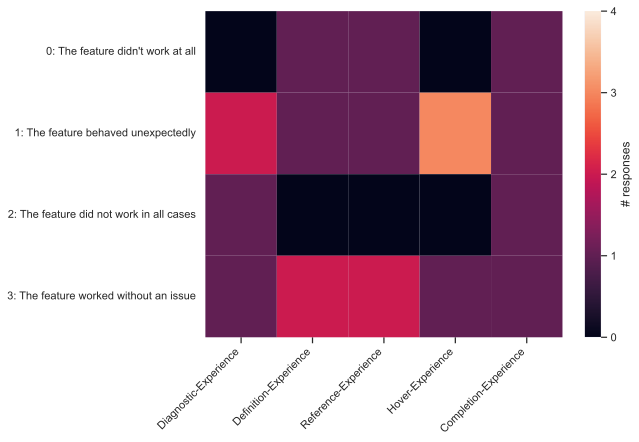
\includegraphics[width=0.5\textwidth,height=\textheight]{log_analysis/figures/results-comp-experience}\label{fig:results-comp-experience}}
\subfloat[Number of votes for each satisfaction category and
feature]{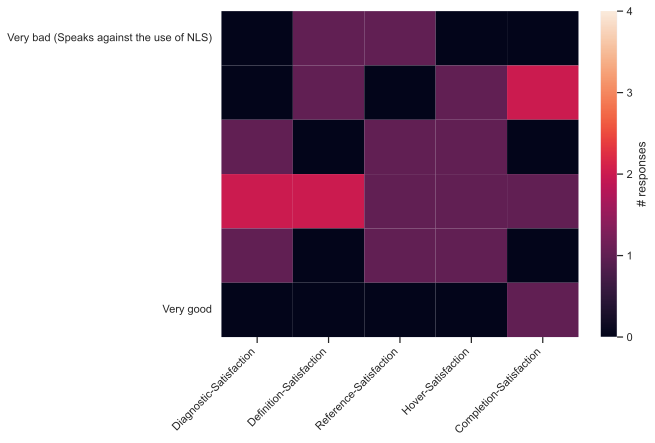
\includegraphics[width=0.5\textwidth,height=\textheight]{log_analysis/figures/results-comp-satisfaction}\label{fig:results-comp-satisfaction}}

\subfloat[Number of votes for each expectation category and
feature]{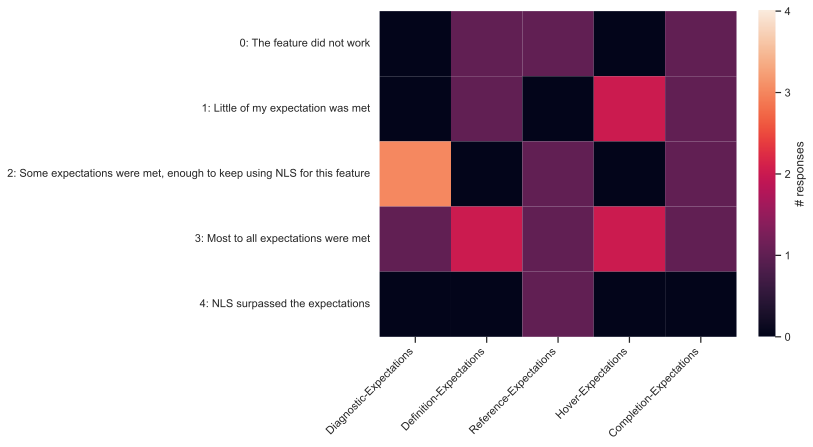
\includegraphics[width=0.75\textwidth,height=\textheight]{log_analysis/figures/results-comp-expectations}\label{fig:results-comp-expectations}}

\caption[{User responses regarding general experience, fulfillment of
expectations and general satisfaction.}]{User responses regarding
general experience, fulfillment of expectations and general
satisfaction.}

\label{fig:expe-survey-results}

\end{pandoccrossrefsubfigures}

Figures \ref{fig:results-comp-experience},
\ref{fig:results-comp-satisfaction}, \ref{fig:results-comp-expectations}
show the turnout of three items from the survey for each of the relevant
features. Neither of them exhibits clear trends with positive and
negative results distributed almost evenly between positive and negative
sentiment.

The first graph (fig.~\ref{fig:results-comp-experience}) represents the
participants' general experience with the relevant features. It shows
that each feature worked without issue in at least one instance. Yet,
three features were reported to not work at all and no feature left the
users unsurprised. Users found the hover and diagnostic features to
behave particularly unexpectedly.

In the second item of each feature, the survey asked the subjects to
rate the quality of the language server based on their expectations.
Figure \ref{fig:results-comp-expectations} summarizes the results. In
agreement with the first graph, one user was unable to use at least
three features entirely. The majority of responses show that NLS met its
user's expectations at least partially. The results are however highly
polarized as the Jump-to-Definition and Hover features demonstrate; Each
received equally many votes for being inapt and fully able to hold up to
the participants expectations at the same time. Other features were left
with a uniformly distributed assessment (e.g.~Completion and
Find-References). The clearest result was achieved by the Diagnostics
feature, which received a slight but uncontested positive sentiment.

The general satisfaction with each feature was answered in the same
polarized manner as seen in fig.~\ref{fig:results-comp-satisfaction}. A
slight majority of responses falls into the upper half of the possible
spectrum. Two of the features reported without function in the preceding
questions were given the lowest possible rating.

\hypertarget{sec:hover-res}{%
\paragraph{Hover}\label{sec:hover-res}}

As apparent in (fig.~\ref{fig:results-comp-experience}), most
participants experienced unexpected behavior by the LSP when using the
hover functionality. In the comments, extraneous debug output and
incorrect displaying of the output by the IDE are pointed out as
concrete examples. However, one answer suggests that the feature was
working with ``usually useful'' output.

\hypertarget{sec:diagnostics-res}{%
\paragraph{Diagnostics}\label{sec:diagnostics-res}}

While the diagnostics shown by NLS appear to behave unexpectedly for
some users in fig.~\ref{fig:results-comp-experience}, no user felt
deterred from keep using NLS for it as displayed in
fig.~\ref{fig:results-comp-expectations}. Some respondents praised the
``quick'' and ``direct feedback'' as well as the visual error markers
pointing to the exact locations of possible issues. On the contrary,
others mentioned ``unclear messages'' and pointed out that contracts
were not checked by the Language Server. Moreover, a performance issue
was brought up noting that in some situations NLS ``queues a lot of work
and does not respond.''

\hypertarget{sec:code-completion-res}{%
\paragraph{Code Completion}\label{sec:code-completion-res}}

Comments about the Code Completion feature were unanimously critical.
One participant noted the little gained ``value over the token based
completion built into the editor'' while two others specifically pointed
at ``missing type information and docs.'' Additionally, record field
completion was found to be missing, albeit highly valued.

\hypertarget{sec:document-navigation-res}{%
\paragraph{Document Navigation}\label{sec:document-navigation-res}}

Results and comments about the Go-To-Definition and Find-References were
polarized. Some users experienced unexpected behavior or were unable to
use the feature at all (cf. fig.~\ref{fig:results-comp-experience}).
Similarly, the comments on one hand suggest that ``the feature works
well and is quick'' while on the other mention inconsistencies and
unavailability. More specifically, cross file navigation was named an
important missing feature.

\hypertarget{sec:general-performance-res}{%
\paragraph{General Performance}\label{sec:general-performance-res}}

The responses to the general performance suggest that NLS' performance
is largely dependent on its usage. On unmodified files queries were
reported to evaluate ``instantaneously.'' However, modifying files
caused that ``modifications stack up'' causing high CPU usage and
generally ``very slow'' responses. Besides, documentation was reported
as slow to resolve while the server itself was ``generally fast.''

\hypertarget{sec:discussion}{%
\subsubsection{Discussion}\label{sec:discussion}}

\hypertarget{sec:diagnostics-2}{%
\paragraph{Diagnostics}\label{sec:diagnostics-2}}

First, participants criticized sec.~\ref{sec:diagnostics-res} the
diagnostics feature for some unhelpful error messages and specifically
for not taking into account Nickel's hallmark feature, Contracts
sec.~\ref{sec:contracts}. While Contracts are a central element of
Nickel and relied upon to validate data, the language server does not
actually warn about contract breaches. Yet, while contracts and their
application looks similar to types, contracts are a dynamic language
element which are dynamically applied during evaluation. Therefore, it
is not possible to determine whether a value conforms to a contract
without evaluation of the contract. NLS's is integrated with Nickel's
type-checking mechanism which precedes evaluation and provides only a
static representation of the source code. In order to support
diagnostics for contracts NLS would need to locally evaluate arbitrary
code that makes up contracts. However, contracts can not be evaluated
entirely locally as they may transitively depend on other contracts.
This is particularly true for a file's output value. Additionally,
Contracts can implement any sort of complex computation including
unbound recursion. Due to these caveats, evaluating contracts as part of
NLS's analysis implies the evaluation of the entire code which was
considered a possibly significant impact to the performance. As laid out
above evaluating contracts locally is no option either. It is not only
challenging to collect the minimal context of the Contract, the context
may in fact be the entire program. An alternative option is to provide
the ability to apply contracts manually using an LSP feature called
``Code Lenses.'' Code Lenses are displayed by editors as annotations
allowing the user to manually execute an associated action.

\hypertarget{sec:cross-file-navigation}{%
\paragraph{Cross File Navigation}\label{sec:cross-file-navigation}}

In both cases \texttt{Jump-To-Definition} and \texttt{Find-References}
surveyed users requested support for cross file navigation. In
particular, finding the definition of a record field of an imported
record should navigate the editor to the respective file as symbolized
in lst.~\ref{lst:imported-record-access}.

\begin{codelisting}

\caption{Minimal example of cross file referencing}

\hypertarget{lst:imported-record-access}{%
\label{lst:imported-record-access}}%
\begin{verbatim}
// file_a.ncl

let b = import "./b.ncl" in b.field
                              |
                              +------+
                                     |
-----------------------------------  |
                                     |
// file_b.ncl                        |
                                     |
{                                    |
  field = "field value";             |
}  ^                                 |
   +---------------------------------+
\end{verbatim}

\end{codelisting}

The resolution of imported values is done at evaluation time, the AST
therefore only contains nodes representing the concept of an import but
no not reference elements of that file. NLS does ingest the AST without
resolving these imports manually. The type checking module underlying
NLS still recurses into imported files to check their formal
correctness. As a result it would be possible for a NLS to resolve these
links as an additional step in the post-processing by either inserting
artificial linearization items sec.~\ref{sec:linearization} or merging
both files' linearization entirely.

\hypertarget{sec:autocompletion}{%
\paragraph{Autocompletion}\label{sec:autocompletion}}

Another criticized element of NLS was the autocompletion feature. In the
survey, participants mentioned the lack of additional information and
distinction of elements as well as NLS inability to provide completion
for record fields. In Nickel, record access is declared by a period. An
LSP client can be configured to ask for completions when such an access
character is entered additionally to manual requests by the user. The
language server is then responsible to provide a list of completion
candidates depending on the context, i.e.~the position. {[}Section
\#sec:completion{]} describes how NLS resolves this kind of request. NLS
just lists all identifiers of declarations that are in scope at the
given position. Notably, it does not take the preceding element into
account as additional context. To support completing records, the server
must first be aware of separating tokens such as the period symbol,
check whether the current position is part of a token that is preceded
by a separator and finally resolve the parent element to a record.

\hypertarget{sec:quantitative}{%
\subsection{Quantitative}\label{sec:quantitative}}

The quantitative evaluation focuses on the performance characteristics
of NLS. As described in sec.~\ref{sec:quantitative-methods} a tracing
module was embedded into the NLS binary which recorded the runtime
together with the size of the analyzed data, i.e., the number of
linearization items sec.~\ref{sec:linearization} or size of the analyzed
file. This section will first introduce the dataset before looking at
the general performance and finally looking into particular cases.

\hypertarget{sec:dataset}{%
\subsubsection{Dataset}\label{sec:dataset}}

The underlying data set consists of 16761 unique trace records,
contributed by the lead developer of Nickel. The traces were generated
during the work on different Nickel files of varying size during the
course of one day. It is a record of both the development of entire new
files and work on a bigger Nickel based project.

Since the \texttt{textDocument/didOpen} method is executed on every
update of the source, it greatly outnumbers the other events. The final
distribution of methods traced is:

\begin{longtable}[]{@{}lll@{}}
\caption{Number of traces per LSP method}\tabularnewline
\toprule
Method & count & linearization based \\
\midrule
\endfirsthead
\toprule
Method & count & linearization based \\
\midrule
\endhead
\texttt{textDocument/didOpen} & 13436 & no \\
\texttt{textDocument/completion} & 2981 & yes \\
\texttt{textDocument/hover} & 227 & yes \\
\texttt{textDocument/definition} & 68 & yes \\
\texttt{textDocument/references} & 49 & yes \\
& & \\
total & 16761 & \\
\bottomrule
\end{longtable}

\begin{pandoccrossrefsubfigures}

\subfloat[Distribution of linearization based LSP
requests]{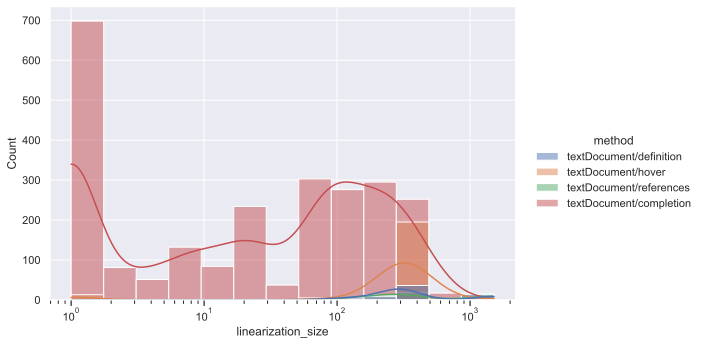
\includegraphics[width=0.5\textwidth,height=\textheight]{log_analysis/figures/distribution-by-lin-size}\label{fig:distribution-by-lin-size}}
\subfloat[Distribution of file analysis
requests]{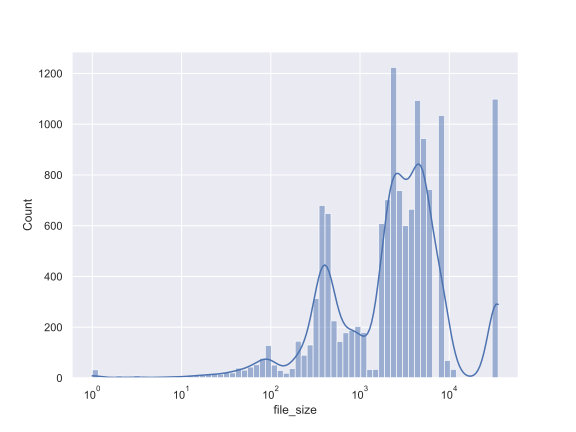
\includegraphics[width=0.5\textwidth,height=\textheight]{log_analysis/figures/distribution-by-file-size}\label{fig:distribution-by-file-size}}

\subfloat[Empirical Cumulative Distribution of linearization based LSP
requests]{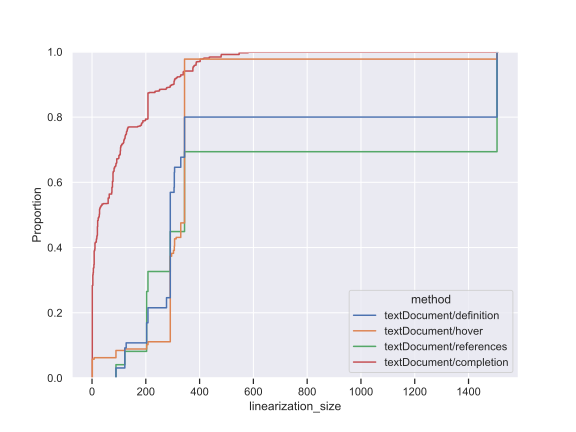
\includegraphics[width=0.5\textwidth,height=\textheight]{log_analysis/figures/ecdf-by-lin-size}\label{fig:ecdf-by-lin-size}}
\subfloat[Empirical Cumulative Distribution of file analysis
requests]{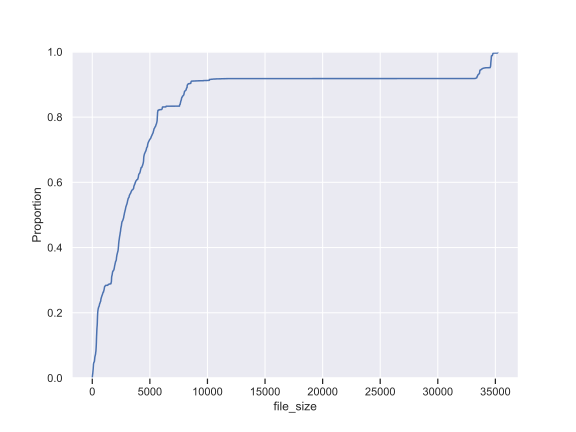
\includegraphics[width=0.5\textwidth,height=\textheight]{log_analysis/figures/ecdf-by-file-size}\label{fig:ecdf-by-file-size}}

\caption[{Estimated distribution and empirical cumulative distributions
of traced method calls.}]{Estimated distribution and empirical
cumulative distributions of traced method calls.}

\label{fig:distributions}

\end{pandoccrossrefsubfigures}

Figures \ref{fig:distribution-by-lin-size} break up these numbers by
method and linearization size or file size respectively. The
linearization is the linear representation of an enriched AST. It is
explained in great detail in sec.~\ref{sec:linearization}. The first
figure shows a peak number of traces for completion events between \(0\)
to \(1\) linearization items as well as local maxima around a
linearization size of \(20\) to \(30\) and sustained usage of completion
requests in files of \(90-400\) items. Similar to the completion
requests (but well outnumbered in total counts), other methods were used
mainly in the range between \(200\) and \(400\) linearization items. A
visualization of the Empirical Cumulative Distribution Function (ECDF)
figs.~\ref{fig:ecdf-by-lin-size}, \ref{fig:ecdf-by-file-size}
corroborates these findings. Moreover, it shows an additional hike of
Jump-to-Definition and Find-References calls at on files with around
1500 linearization items. The findings for linearization based methods
line up with those depicting linearization events (identified as
\texttt{textDocument/didOpen}). An initial peak referring to rather
small input files between \(300\) and \(400\) bytes in size is followed
by a sustained usage of the NLS on files with \(2\) to \(6\) kilobytes
of content topped with a final application on \(35\) kilobyte large
data.

\hypertarget{sec:big-picture-latencies}{%
\subsubsection{Big Picture Latencies}\label{sec:big-picture-latencies}}

\begin{figure}
\hypertarget{fig:boxplot-latencies}{%
\centering
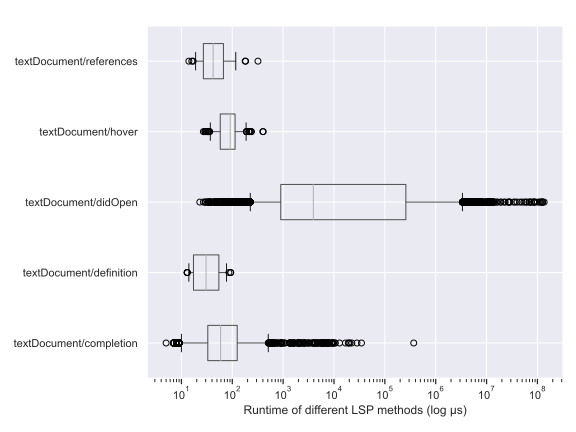
\includegraphics{log_analysis/figures/boxplot-latencies}
\caption{Statistical runtime of different LSP
methods}\label{fig:boxplot-latencies}
}
\end{figure}

Comparing the runtime of the individual methods alone in
fig.~\ref{fig:boxplot-latencies}, reveals three key findings. First, all
linearization based methods exhibit a sub-millisecond latency in at
least \(95%
\) of all invocations and median response times of less than \(100µs\)
However, maximum latencies of completion invocations reached tens of
milliseconds and in one recorded case about \(300ms\). Finally, document
linearization as associated with the \texttt{textDocument/didOpen}
method shows a great range with maxima of \(1.5 * 10^5µs\) (about
\(2.5\) minutes) and a generally greater interquartile range spanning
more than two orders of magnitude.

\hypertarget{sec:special-cases}{%
\subsubsection{Special cases}\label{sec:special-cases}}

\begin{pandoccrossrefsubfigures}

\subfloat[Runtime latencies of completion requests at different
linearization
sizes]{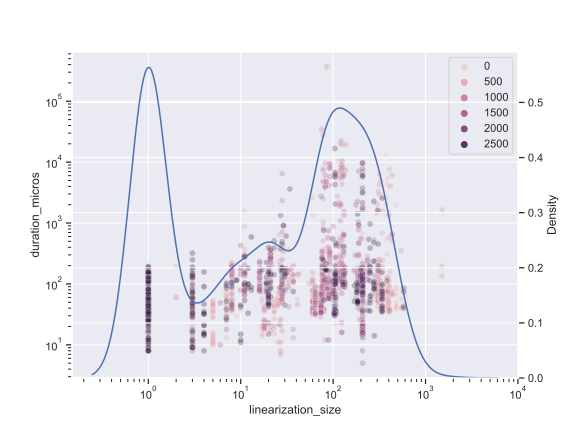
\includegraphics[width=0.5\textwidth,height=\textheight]{log_analysis/figures/correlation-completions}\label{fig:correlation-completions}}
\subfloat[Runtime latencies of hover requests at different linearization
sizes]{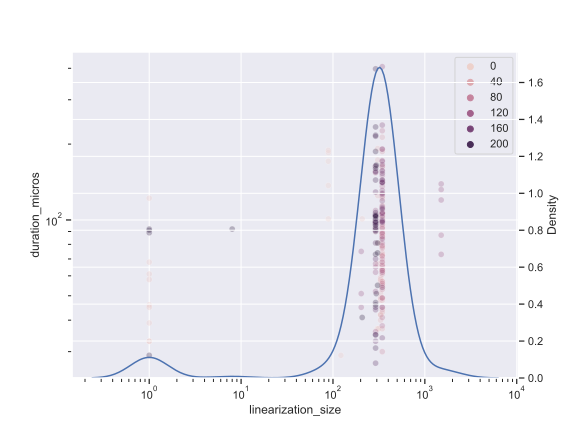
\includegraphics[width=0.5\textwidth,height=\textheight]{log_analysis/figures/correlation-hovers}\label{fig:correlation-hovers}}

\subfloat[Runtime latencies of find-references requests at different
linearization
sizes]{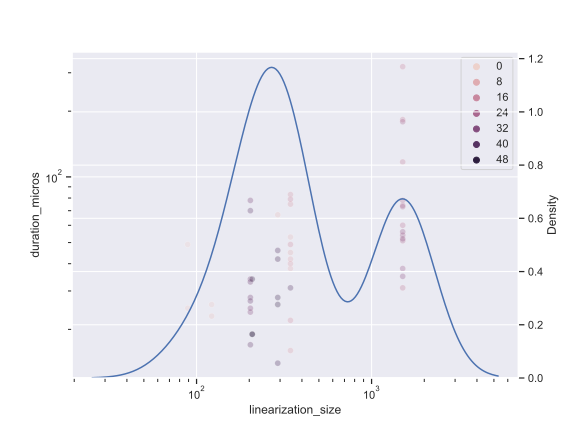
\includegraphics[width=0.5\textwidth,height=\textheight]{log_analysis/figures/correlation-references}\label{fig:correlation-references}}
\subfloat[Runtime latencies of jump-to-definition requests at different
linearization
sizes]{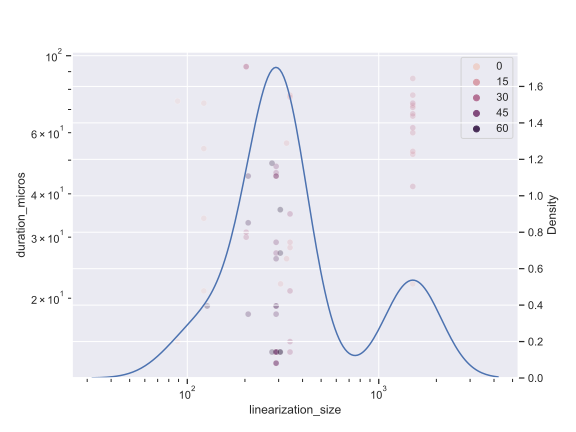
\includegraphics[width=0.5\textwidth,height=\textheight]{log_analysis/figures/correlation-definitions}\label{fig:correlation-definitions}}

\caption[{Runtime latencies of different linearization based
methods}]{Runtime latencies of different linearization based methods}

\label{fig:correlation-linearization-methods}

\end{pandoccrossrefsubfigures}

\begin{figure}
\hypertarget{fig:correlation-opens}{%
\centering
\includegraphics[width=0.5\textwidth,height=\textheight]{log_analysis/figures/correlation-opens}
\caption{Runtime latencies of file update handling at different file
sizes}\label{fig:correlation-opens}
}
\end{figure}

Setting the runtime of completion requests in relation to the
linearization size on which the command was performed shows no clear
correlation between the dimensions. In fact the correlation coefficient
between both variables measures \(0.01617\) on a linear scale and
\(0.26\) on a \(\log_{10}\log_{10}\) scale. Instead, vertical columns
stand out in the correlation graph
fig.~\ref{fig:correlation-completions}. The height of these columns
varies from one to five orders of magnitude. The item density shows that
especially high columns form whenever the server receives a higher load
of requests. Additionally, color coding the individual requests by time
reveals that the trace points of each column were recorded at a short
time interval. Applying the same analysis to the other methods in
figs.~\ref{fig:correlation-hovers}, \ref{fig:correlation-references}, \ref{fig:correlation-definitions}
returns similar findings, although the columns remain more compact in
comparison to the Completions method. In case of the \texttt{didOpen}
method columns are clearly visible too fig.~\ref{fig:correlation-opens}.
However, here they appear leaning as suggesting an increase in
computation time as the file grows during a single series of changes to
the file.

\hypertarget{sec:discussion-1}{%
\subsubsection{Discussion}\label{sec:discussion-1}}

In the experience survey performance was pointed out as a potential
issue. Especially in connection with the diagnostics and hover feature.
NLS was described to ``queue a lot of work and not respond'' and show
different performance signatures depending on its usage. While commands
resolved ``instantaneously'' on unmodified files, editing a file causes
high CPU usage and generally ``very slow'' responses. An analysis of the
measured runtime of \(16761\) requests confirmed that observation. Both
Hover and Update requests showed a wide range of latencies with some
reaching more than two minutes. However, the data distribution also
confirmed that latencies for most requests except \texttt{didOpen} are
distributed well below one millisecond. The \texttt{didOpen} requests
which are associated with the linearization process (c.f.
sec.~\ref{sec:linearization}) peak around \(1ms\) but longer latencies
remain frequent: fig.~\ref{fig:distribution-latencies}. Looking deeper
into the individual features, reveals signs of the aforementioned
``stacking.'' As discussed in sec.~\ref{sec:special-cases} subsequent
requests exhibit increasing processing times especially during peak
usage.

\begin{figure}
\hypertarget{fig:distribution-latencies}{%
\centering
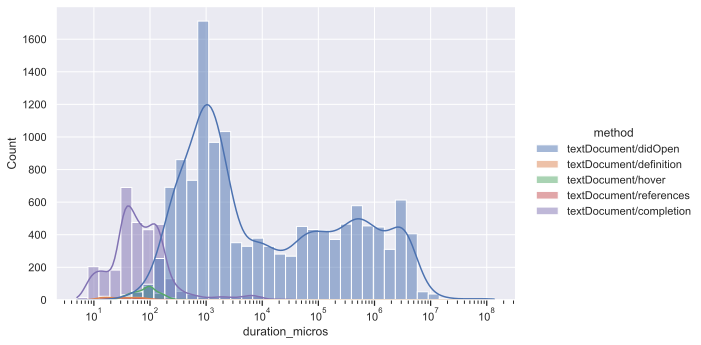
\includegraphics[width=0.66\textwidth,height=\textheight]{log_analysis/figures/distribution-latencies}
\caption{Distribution of latencies by request
type}\label{fig:distribution-latencies}
}
\end{figure}

This behavior is caused by the architecture of the LSP and NLS'
processing method. The Language Server Protocol is a synchronous
protocol which requires the processing of all requests FIFO order. In
effect, every request is delayed until previous requests are handled.
This effect is particularly strong as the server is faced with a high
volume. In the case of the trace for \texttt{didOpen} events the delay
effect is greater than for other methods as \texttt{didOpen} is
associated with a full analysis of the entire file. NLS architecture is
heavily influenced by the desire to reuse as many elements of the Nickel
runtime as possible to maintain feature parity with the evolving
language core. Consequently, file updates invoke a complete eager
analysis of the contents; The entire document is parsed, type checked
and recorded to a linearization every time. In contrast, all other
methods rely on the linearization of a document which allows them to use
a binary search to efficiently lookup elements in logarithmic time.
Additionally, all requests regardless of their type are subject to the
same queue. Given that \texttt{didOpen} requests make up \(>80%
\) of the recorded events, suggests that other events are heavily slowed
down collaterally.

Multiple ways exist to address this issue by reducing the average queue
size. The most approachable way to reduce queue sizes is to reduce the
number of requests the server needs to handle. The \texttt{didOpen}
trace elements actually represents the joint processing path of initial
file openings, and changes. NLS configures clients to signal changes
both on save and following editor defined ``change.'' The fact that it
is the editor's responsibility to define what constitutes a change means
that some editors send invoke the server on every key press. In
fig.~\ref{fig:distribution-latencies} signs for such a behavior can be
seen as local increases of processing time as the document grows. Hence,
restricting analysis to happen only as the user saves the document could
potentially reduce the load of requests substantially. Yet, many users
preferred automatic processing to happen while they type. To server this
pattern, NLS could implement a debouncing mechanism for the processing
of document changes. The messages associated to document changes and
openings are technically no requests but notifications. The
specification of JSON-RPC which the LSP is based on defines that
notifications are not allowing a server response. Clients can not rely
on the execution of associated procedures. In effect, a language server
like NLS, where each change notification contains the entire latest
document, may skip the processing of changes. In practice, NLS could
skip such queue items if a more recent version of the file is notified
later in the queue. The queue size can also be influenced by reducing
the processing time. Other language servers such as the rust-analyzer
{[}61{]} chose to process documents lazily. Update requests
incrementally change an internal model which other requests use as a
basis to invoke targeted analysis, resolve elements and more. The entire
model is based on in incremental computation model which automates
memorization of requests. This method however requires rust-analyzer to
reimplement core components of rust to support incrementally. Therefore,
if one accepts to implement an incremental model of Nickel (including
parsing and type checking) to enable incremental analysis in NLS,
switching to a lazy model is a viable method to reduce the processing
time of change notifications and shorten the queue.

\hypertarget{sec:conclusion}{%
\chapter{Conclusion}\label{sec:conclusion}}

This chapter summarizes the outcomes of the research underlying this
thesis and how they answer the research questions raised in
sec.~\ref{sec:research-questions}. Moreover, it will discuss the
limitations of the Language Server implementation as discovered in
sec.~\ref{sec:evaluation}. Finally, it suggests some short and long term
research opportunities in the field of language servers.

\hypertarget{sec:study-outcome}{%
\section{Study Outcome}\label{sec:study-outcome}}

This thesis project was driven by two central research questions:

\begin{quote}
\begin{description}
\item[RQ.1]
\begin{enumerate}
\def\labelenumi{\alph{enumi})}
\tightlist
\item[]
\item
  How to develop a language server for a new language that
\end{enumerate}

\begin{enumerate}
\def\labelenumi{\alph{enumi})}
\setcounter{enumi}{1}
\tightlist
\item
  satisfies its users' needs while being performant enough not to slow
  them down?
\end{enumerate}
\item[RQ.2]
How can we assess the implementation both quantitatively based on
performance measures and qualitatively based on user satisfaction?
\end{description}
\end{quote}

Chapter \ref{sec:design-and-implementation} introduced an approach to
implement language server based on the Language Server Protocol. Section
\ref{sec:high-level-architecture} describes how the NLS consists of
three modules: A generic Language Server Interface, an implementation of
the interface for the target language Nickel as well as minimal
adaptions to Nickel itself. The architecture aims to provide
generalizability to other languages by replacing the implementation of
the Language Server Interface.

At the core of the interface stands the Linearization -- a data
structure that represents the syntactic structure of a program linearly
as opposed to in a tree-like structure. However, elements can contain
references (e.g.~variable usages reference elements representing the
corresponding declaration), constituting a graph on top of the linear
structure. The data structure is populated using a single tree
traversal. In NLS, this traversal is implemented by Nickel's type
checking which was modified to pass typed AST nodes into the
linearization. The linearization allows efficient access to analysis
results for arbitrary positions. NLS implements handlers for several
requests of the LSP that exploit this property to provide capabilities
like Jump-to-Declaration, Hover and Auto-Completion as detailed in
sec.~\ref{sec:lsp-server-implementation}.

While sec.~\ref{sec:design-and-implementation} answers RQ.1a), to answer
RQ.1b) its ability to efficiently provide satisfying results had to be
assessed objectively. This research relies on both qualitative and
quantitative data to address RQ.1b). Chapter \ref{sec:evaluation}
describes the process of the evaluation which answers RQ.2. Tweag
employees helped to evaluate the NLS taking part in a workshop and
sharing their expectations and experiences through separate surveys. The
data showed fairly polarized satisfaction with the tool.

\hypertarget{sec:limitations}{%
\section{Limitations}\label{sec:limitations}}

While the NLS project yielded a working and under good conditions
performant implementation of the LSP, limitations standing in the way of
its adaption remain. During the evaluation, users criticized that some
features were only usable in a limited scope. References to imported
files were not followed and autocompletion only worked for top level
variable names. Moreover, performance issues were reported. A
quantitative analysis of the latencies shown by the NLS supported the
performance concerns brought up in the surveys. Processing files can be
observed to be slower as file sizes increase. At the same time what
constitutes a ``file change'' is an implementation detail of the LSP
client and may issues as frequent as on every keystroke. Since requests
are processed synchronously, files are needlessly processes multiple
times. The limitations are discussed in detail in
sec.~\ref{sec:discussion}.

\hypertarget{sec:future-work}{%
\section{Future Work}\label{sec:future-work}}

The apart from discussing the shortcoming found during the evaluation,
sec.~\ref{sec:discussion} brings up several opportunities around
criticized features for future research and implementation. Improving
the highly demanded features such as Auto-Completion and cross file
references are easy targets for work in the short term future.

Advancing over simple feature additions, future work should look into
improving performance by reducing server load. Alternatively
implementing incremental processing capabilities to the linearization
could be a more involved but more sustainable research. This way only
the changed contents of files would be transmitted and integrated into
NLS's data model. It's open how type checking and other diagnostics can
be integrated into this process.

Additionally, some platforms start to use the static Language Server
Index Format (LSIF) to provide code aware navigation in static contexts
such as websites where running a language server is impractical. The
Linearization already represents a static view on a file that underlies
all LSP methods. Hence, it is conceivable to implement a translation
into LSIF to be used by supported platforms.

Finally, while the project is structured to be transferred to other
languages, this feature has not been assessed. Future projects should
include the implementation of a language server based on the
abstractions presented here. Only such work could verify the
generalizability of the architecture underlying NLS.

\hypertarget{sec:analysis-of-the-impact-on-the-society-ethics-and-sustainability}{%
\section{Analysis of the Impact on the Society, Ethics and
Sustainability}\label{sec:analysis-of-the-impact-on-the-society-ethics-and-sustainability}}

As a tool targeting exclusively software developers, and in reality only
a subset thereof, the direct impact on the society as a whole this tool
has, is negligible. This project aims to (1) improve the workflow of
Nickel Developers directly and (b) enable developers to provide the same
to their peers using another language. Therefore, the impact of this
tool is limited to an improved productivity and work experience of the
developers using this work's artifacts.

Nickel as well as its language server and the related academic work
presented here are publicly available. The creators of that work are
hence unable to control or assess the application of their tools,
whether ethical or not. Considering privacy, the project associated to
this work, NLS, includes an optional usage logging mode which has access
to a user's entire interaction with the tool including source code, file
names, etc. However, no personal data is exposed, and the logs are never
transferred from the user's machine.

In terms of sustainability, the performance analysis reported in
{[}\#sec:quantitative{]} showed that NLS currently, processes requests
very inefficiently. To the user this appears as surging latencies as
well as significantly increased power consumption due to constant
(unnecessary) computation.

\hypertarget{sec:references}{%
\chapter*{References}\label{sec:references}}
\addcontentsline{toc}{chapter}{References}

\hypertarget{refs}{}
\begin{CSLReferences}{0}{0}
\leavevmode\vadjust pre{\hypertarget{ref-bourMerlinLanguageServer2018a}{}}%
\CSLLeftMargin{{[}1{]} }
\CSLRightInline{F. Bour, T. Refis, and G. Scherer, {``Merlin: {A
Language Server} for {OCaml} ({Experience Report}),''} \emph{Proceedings
of the ACM on Programming Languages}, vol. 2, no. ICFP, pp. 1--15, Jul.
2018, doi: \href{https://doi.org/10.1145/3236798}{10.1145/3236798}.
{[}Online{]}. Available: \url{http://arxiv.org/abs/1807.06702}.
{[}Accessed: Nov. 12, 2021{]}}

\leavevmode\vadjust pre{\hypertarget{ref-sloaneMontoDisintegratedDevelopment2014}{}}%
\CSLLeftMargin{{[}2{]} }
\CSLRightInline{A. M. Sloane, M. Roberts, S. Buckley, and S. Muscat,
{``Monto: {A Disintegrated Development Environment},''} in
\emph{Software {Language Engineering}}, 2014, pp. 211--220, doi:
\href{https://doi.org/10.1007/978-3-319-11245-9_12}{10.1007/978-3-319-11245-9\_12}.
}

\leavevmode\vadjust pre{\hypertarget{ref-sourcegraphLangserverOrg}{}}%
\CSLLeftMargin{{[}3{]} }
\CSLRightInline{Sourcegraph, {``Langserver.org.''} {[}Online{]}.
Available: \url{https://langserver.org/}. {[}Accessed: Apr. 27, 2022{]}}

\leavevmode\vadjust pre{\hypertarget{ref-microsoftLanguageServers}{}}%
\CSLLeftMargin{{[}4{]} }
\CSLRightInline{Microsoft, {``Language {Servers}.''} {[}Online{]}.
Available:
\url{https://microsoft.github.io/language-server-protocol/implementors/servers/}.
{[}Accessed: May 01, 2022{]}}

\leavevmode\vadjust pre{\hypertarget{ref-meyerovichEmpiricalAnalysisProgramming2013}{}}%
\CSLLeftMargin{{[}5{]} }
\CSLRightInline{L. A. Meyerovich and A. S. Rabkin, {``Empirical analysis
of programming language adoption,''} in \emph{Proceedings of the 2013
{ACM SIGPLAN} international conference on {Object} oriented programming
systems languages \& applications}, Oct. 2013, pp. 1--18, doi:
\href{https://doi.org/10.1145/2509136.2509515}{10.1145/2509136.2509515}
{[}Online{]}. Available: \url{https://doi.org/10.1145/2509136.2509515}.
{[}Accessed: Dec. 21, 2021{]}}

\leavevmode\vadjust pre{\hypertarget{ref-Nickel2022}{}}%
\CSLLeftMargin{{[}6{]} }
\CSLRightInline{{``Nickel.''} Tweag, May 2022 {[}Online{]}. Available:
\url{https://github.com/tweag/nickel}. {[}Accessed: May 24, 2022{]}}

\leavevmode\vadjust pre{\hypertarget{ref-OCamlLSP2022}{}}%
\CSLLeftMargin{{[}7{]} }
\CSLRightInline{OCaml Community, {``{OCaml Language Server Protocol}
implementation.''} OCaml, Apr. 2022 {[}Online{]}. Available:
\url{https://github.com/ocaml/ocaml-lsp}. {[}Accessed: May 01, 2022{]}}

\leavevmode\vadjust pre{\hypertarget{ref-hessDafnyLanguageServer2019}{}}%
\CSLLeftMargin{{[}8{]} }
\CSLRightInline{M. Hess and T. Kistler, {``Dafny {Language Server
Redesign},''} Srp, HSR Hochschule für Technik Rapperswil, 2019
{[}Online{]}. Available: \url{https://eprints.ost.ch/id/eprint/842/}.
{[}Accessed: Feb. 18, 2022{]}}

\leavevmode\vadjust pre{\hypertarget{ref-kladovExplainingRustanalyzer2021}{}}%
\CSLLeftMargin{{[}9{]} }
\CSLRightInline{A. Kladov, {``Explaining rust-analyzer.''} Nov. 2021
{[}Online{]}. Available:
\url{https://www.youtube.com/playlist?list=PLhb66M_x9UmrqXhQuIpWC5VgTdrGxMx3y}.
{[}Accessed: May 29, 2022{]}}

\leavevmode\vadjust pre{\hypertarget{ref-JSONRPCSpecification2013}{}}%
\CSLLeftMargin{{[}10{]} }
\CSLRightInline{{``{JSON-RPC} 2.0 {Specification},''} {JSON-RPC Working
Group}, Specification, Jan. 2013 {[}Online{]}. Available:
\url{https://www.jsonrpc.org/specification}. {[}Accessed: Dec. 15,
2021{]}}

\leavevmode\vadjust pre{\hypertarget{ref-birrellImplementingRemoteProcedure1984}{}}%
\CSLLeftMargin{{[}11{]} }
\CSLRightInline{A. D. Birrell and B. J. Nelson, {``Implementing {Remote
Procedure Calls},''} \emph{ACM Transactions on Computer Systems}, vol.
2, no. 1, p. 21, 1984. }

\leavevmode\vadjust pre{\hypertarget{ref-microsoftLanguageServerProtocol2020}{}}%
\CSLLeftMargin{{[}12{]} }
\CSLRightInline{Microsoft, {``Language {Server Protocol Specification} -
3.16.''} Dec. 2020 {[}Online{]}. Available:
\url{https://microsoft.github.io/language-server-protocol/specification.html}.
{[}Accessed: Jul. 28, 2021{]}}

\leavevmode\vadjust pre{\hypertarget{ref-w3cExtensibleMarkupLanguage2008}{}}%
\CSLLeftMargin{{[}13{]} }
\CSLRightInline{W3C, {``Extensible {Markup Language} ({XML}) 1.0 ({Fifth
Edition}),''} Specification, Nov. 2008 {[}Online{]}. Available:
\url{https://www.w3.org/TR/2008/REC-xml-20081126/}. {[}Accessed: May 24,
2022{]}}

\leavevmode\vadjust pre{\hypertarget{ref-charollaisECMA4042ndEdition2017}{}}%
\CSLLeftMargin{{[}14{]} }
\CSLRightInline{P. Charollais, {``{ECMA-404}, 2nd edition, {December}
2017,''} p. 16, 2017. }

\leavevmode\vadjust pre{\hypertarget{ref-YAMLAinMarkup}{}}%
\CSLLeftMargin{{[}15{]} }
\CSLRightInline{{``{YAML Ain}'t {Markup Language}
({YAML}\texttrademark ) revision 1.2.2''} {[}Online{]}. Available:
\url{https://yaml.org/spec/1.2.2/}. {[}Accessed: May 24, 2022{]}}

\leavevmode\vadjust pre{\hypertarget{ref-Pereira2016}{}}%
\CSLLeftMargin{{[}16{]} }
\CSLRightInline{C. R. Pereira, {``Managing modules with {NPM},''} in
\emph{Building {APIs} with {Node}.js}, {Berkeley, CA}: {Apress}, 2016,
pp. 9--13 {[}Online{]}. Available:
\url{https://doi.org/10.1007/978-1-4842-2442-7_3}}

\leavevmode\vadjust pre{\hypertarget{ref-Varanasi2014}{}}%
\CSLLeftMargin{{[}17{]} }
\CSLRightInline{B. Varanasi and S. Belida, {``Maven project basics,''}
in \emph{Introducing maven}, {Berkeley, CA}: {Apress}, 2014, pp. 23--36
{[}Online{]}. Available:
\url{https://doi.org/10.1007/978-1-4842-0841-0_4}}

\leavevmode\vadjust pre{\hypertarget{ref-adermannComposer}{}}%
\CSLLeftMargin{{[}18{]} }
\CSLRightInline{N. Adermann and J. Boggiano, {``Composer.''}
{[}Online{]}. Available: \url{https://getcomposer.org/}. {[}Accessed:
May 24, 2022{]}}

\leavevmode\vadjust pre{\hypertarget{ref-Vemula2017}{}}%
\CSLLeftMargin{{[}19{]} }
\CSLRightInline{R. Vemula, {``Configuring a continuous build with travis
{CI},''} in \emph{Real-time web application development : {With
ASP}.{NET} core, {SignalR}, docker, and azure}, {Berkeley, CA}:
{Apress}, 2017, pp. 489--508 {[}Online{]}. Available:
\url{https://doi.org/10.1007/978-1-4842-3270-5_13}}

\leavevmode\vadjust pre{\hypertarget{ref-hellerAutomatingWorkflowsGitHub2021}{}}%
\CSLLeftMargin{{[}20{]} }
\CSLRightInline{P. Heller, \emph{Automating {Workflows} with {GitHub
Actions}: {Automate} software development workflows and seamlessly
deploy your applications using {GitHub Actions}}. {Packt Publishing},
2021. }

\leavevmode\vadjust pre{\hypertarget{ref-arefeen2019continuous}{}}%
\CSLLeftMargin{{[}21{]} }
\CSLRightInline{M. S. Arefeen and M. Schiller, {``Continuous integration
using gitlab,''} \emph{Undergraduate Research in Natural and Clinical
Science and Technology Journal}, vol. 3, pp. 1--6, 2019. }

\leavevmode\vadjust pre{\hypertarget{ref-burnsKubernetesRunning}{}}%
\CSLLeftMargin{{[}22{]} }
\CSLRightInline{B. Burns, J. Beda, and K. Hightower, {``Kubernetes: {Up}
and {Running},''} p. 277. }

\leavevmode\vadjust pre{\hypertarget{ref-Jangla2018}{}}%
\CSLLeftMargin{{[}23{]} }
\CSLRightInline{K. Jangla, {``Docker compose,''} in \emph{Accelerating
development velocity using docker: {Docker} across microservices},
{Berkeley, CA}: {Apress}, 2018, pp. 77--98 {[}Online{]}. Available:
\url{https://doi.org/10.1007/978-1-4842-3936-0_6}}

\leavevmode\vadjust pre{\hypertarget{ref-pezoaFoundationsJSONSchema2016}{}}%
\CSLLeftMargin{{[}24{]} }
\CSLRightInline{F. Pezoa, J. L. Reutter, F. Suarez, M. Ugarte, and D.
Vrgoč, {``Foundations of {JSON Schema},''} in \emph{Proceedings of the
25th {International Conference} on {World Wide Web}}, Apr. 2016, pp.
263--273, doi:
\href{https://doi.org/10.1145/2872427.2883029}{10.1145/2872427.2883029}
{[}Online{]}. Available: \url{https://doi.org/10.1145/2872427.2883029}.
{[}Accessed: May 24, 2022{]}}

\leavevmode\vadjust pre{\hypertarget{ref-w3cW3CXMLSchema}{}}%
\CSLLeftMargin{{[}25{]} }
\CSLRightInline{W3C, {``{W3C XML Schema Definition Language} ({XSD}) 1.1
{Part} 1: {Structures}.''} {[}Online{]}. Available:
\url{https://www.w3.org/TR/xmlschema11-1/}. {[}Accessed: Jan. 02,
2022{]}}

\leavevmode\vadjust pre{\hypertarget{ref-Webpacka}{}}%
\CSLLeftMargin{{[}26{]} }
\CSLRightInline{{``Webpack.''} JS Foundation {[}Online{]}. Available:
\url{https://webpack.js.org/}. {[}Accessed: May 24, 2022{]}}

\leavevmode\vadjust pre{\hypertarget{ref-macraeVueJsRunning2018}{}}%
\CSLLeftMargin{{[}27{]} }
\CSLRightInline{C. Macrae, \emph{Vue.js: {Up} and {Running}: {Building
Accessible} and {Performant Web Apps}}, 1st edition. {Sebastopol,
California}: {O'Reilly Media}, 2018. }

\leavevmode\vadjust pre{\hypertarget{ref-martelliDistributingExtensionsPrograms}{}}%
\CSLLeftMargin{{[}28{]} }
\CSLRightInline{A. Martelli, A. Ravenscroft, and S. Holden,
\emph{Distributing {Extensions} and {Programs}}. {[}Online{]}.
Available:
\url{https://learning.oreilly.com/library/view/python-in-a/9781491913833/ch25.html}.
{[}Accessed: May 24, 2022{]}}

\leavevmode\vadjust pre{\hypertarget{ref-DhallConfigurationLanguage}{}}%
\CSLLeftMargin{{[}29{]} }
\CSLRightInline{{``The {Dhall} configuration language.''} Dhall
{[}Online{]}. Available: \url{https://dhall-lang.org/}. {[}Accessed:
Jan. 01, 2022{]}}

\leavevmode\vadjust pre{\hypertarget{ref-CUE}{}}%
\CSLLeftMargin{{[}30{]} }
\CSLRightInline{{``{CUE}.''} Cue Language Community {[}Online{]}.
Available: \url{https://cuelang.org/}. {[}Accessed: Jan. 01, 2022{]}}

\leavevmode\vadjust pre{\hypertarget{ref-JsonnetDataTemplating}{}}%
\CSLLeftMargin{{[}31{]} }
\CSLRightInline{{``Jsonnet - {The Data Templating Language}.''} Code
owned by Google {[}Online{]}. Available: \url{https://jsonnet.org/}.
{[}Accessed: Jan. 01, 2022{]}}

\leavevmode\vadjust pre{\hypertarget{ref-beyerSiteReliabilityWorkbook2018}{}}%
\CSLLeftMargin{{[}32{]} }
\CSLRightInline{B. Beyer, N. R. Murphy, D. K. Rensin, K. Kawahara, and
S. Thorne, \emph{The {Site Reliability Workbook}: {Practical Ways} to
{Implement SRE}}. {"O'Reilly Media, Inc."}, 2018. }

\leavevmode\vadjust pre{\hypertarget{ref-Nix2022}{}}%
\CSLLeftMargin{{[}33{]} }
\CSLRightInline{{``Nix.''} Nix/Nixpkgs/NixOS, May 2022 {[}Online{]}.
Available: \url{https://github.com/NixOS/nix}. {[}Accessed: May 01,
2022{]}}

\leavevmode\vadjust pre{\hypertarget{ref-NixOps2022}{}}%
\CSLLeftMargin{{[}34{]} }
\CSLRightInline{{``{NixOps}.''} Nix/Nixpkgs/NixOS, May 2022
{[}Online{]}. Available: \url{https://github.com/NixOS/nixops}.
{[}Accessed: May 24, 2022{]}}

\leavevmode\vadjust pre{\hypertarget{ref-GollumGitbasedWiki2022}{}}%
\CSLLeftMargin{{[}35{]} }
\CSLRightInline{{``Gollum -- {A} git-based {Wiki}.''} Gollum, Jan. 2022
{[}Online{]}. Available: \url{https://github.com/gollum/gollum}.
{[}Accessed: Jan. 04, 2022{]}}

\leavevmode\vadjust pre{\hypertarget{ref-jamesturnbullTerraformBook2016}{}}%
\CSLLeftMargin{{[}36{]} }
\CSLRightInline{James Turnbull, \emph{The {Terraform Book}}. 2016
{[}Online{]}. Available:
\url{https://learning.oreilly.com/library/view/the-terraform-book/9780988820258/}.
{[}Accessed: May 24, 2022{]}}

\leavevmode\vadjust pre{\hypertarget{ref-taylorLearningChef2014}{}}%
\CSLLeftMargin{{[}37{]} }
\CSLRightInline{M. Taylor and S. Vargo, \emph{Learning {Chef}}. 2014
{[}Online{]}. Available:
\url{https://learning.oreilly.com/library/view/learning-chef/9781491945087/}.
{[}Accessed: May 24, 2022{]}}

\leavevmode\vadjust pre{\hypertarget{ref-unit42HighlightsUnit422021}{}}%
\CSLLeftMargin{{[}38{]} }
\CSLRightInline{Unit 42, {``Highlights {From} the {Unit} 42 {Cloud
Threat Report}, {2H} 2021,''} \emph{Unit42}. Sep. 2021 {[}Online{]}.
Available:
\url{https://unit42.paloaltonetworks.com/cloud-threat-report-2h-2021/}.
{[}Accessed: Jan. 04, 2022{]}}

\leavevmode\vadjust pre{\hypertarget{ref-tzvetkovIntegratingAWSCloudFormation2020}{}}%
\CSLLeftMargin{{[}39{]} }
\CSLRightInline{V. Tzvetkov and J. M. Rinaudo, {``Integrating {AWS
CloudFormation} security tests with {AWS Security Hub} and {AWS
CodeBuild} reports,''} \emph{Amazon Web Services}. Sep. 2020
{[}Online{]}. Available:
\url{https://aws.amazon.com/blogs/security/integrating-aws-cloudformation-security-tests-with-aws-security-hub-and-aws-codebuild-reports/}.
{[}Accessed: Jan. 04, 2022{]}}

\leavevmode\vadjust pre{\hypertarget{ref-siekGradualTypingFunctional2006}{}}%
\CSLLeftMargin{{[}40{]} }
\CSLRightInline{J. G. Siek and W. Taha, {``Gradual {Typing} for
{Functional Languages},''} p. 12, 2006. }

\leavevmode\vadjust pre{\hypertarget{ref-hamdaouiRFC001Overriding2022}{}}%
\CSLLeftMargin{{[}41{]} }
\CSLRightInline{Y. Hamdaoui, {``{RFC-001 Overriding},''} {Tweag}, May
2022 {[}Online{]}. Available:
\url{https://github.com/tweag/nickel/blob/f0dc86bd35241ddcb8e9d8482bdc2724ac1b2b19/rfcs/001-overriding.md}.
{[}Accessed: May 24, 2022{]}}

\leavevmode\vadjust pre{\hypertarget{ref-wadlerWellTypedProgramsCan2009}{}}%
\CSLLeftMargin{{[}42{]} }
\CSLRightInline{P. Wadler and R. B. Findler, {``Well-{Typed Programs
Can}'t {Be Blamed},''} in \emph{Programming {Languages} and {Systems}},
vol. 5502, G. Castagna, Ed. {Berlin, Heidelberg}: {Springer Berlin
Heidelberg}, 2009, pp. 1--16 {[}Online{]}. Available:
\url{http://link.springer.com/10.1007/978-3-642-00590-9_1}. {[}Accessed:
May 24, 2022{]}}

\leavevmode\vadjust pre{\hypertarget{ref-desrivieresEclipsePlatformIntegrating2004}{}}%
\CSLLeftMargin{{[}43{]} }
\CSLRightInline{J. des Rivieres and J. Wiegand, {``Eclipse: {A} platform
for integrating development tools. {IBM Systems Journal}, 43(2),
371-383,''} \emph{IBM Systems Journal}, vol. 43, pp. 371--383, Jan.
2004, doi:
\href{https://doi.org/10.1147/sj.432.0371}{10.1147/sj.432.0371}. }

\leavevmode\vadjust pre{\hypertarget{ref-burnetteEclipseIDEPocket2005}{}}%
\CSLLeftMargin{{[}44{]} }
\CSLRightInline{E. Burnette, \emph{Eclipse {IDE}: Pocket guide}, 1st ed.
{Sebastopol, CA}: {O'Reilly}, 2005. }

\leavevmode\vadjust pre{\hypertarget{ref-IntelliJIDEACapable}{}}%
\CSLLeftMargin{{[}45{]} }
\CSLRightInline{{``{IntelliJ IDEA}: {The Capable} \& {Ergonomic Java
IDE} by {JetBrains},''} \emph{JetBrains}. {[}Online{]}. Available:
\url{https://www.jetbrains.com/idea/}. {[}Accessed: May 01, 2022{]}}

\leavevmode\vadjust pre{\hypertarget{ref-VisualStudioIDE}{}}%
\CSLLeftMargin{{[}46{]} }
\CSLRightInline{{``Visual {Studio}: {IDE} and {Code Editor} for
{Software Developers} and {Teams}.''} {[}Online{]}. Available:
\url{https://visualstudio.microsoft.com/}. {[}Accessed: May 01, 2022{]}}

\leavevmode\vadjust pre{\hypertarget{ref-EclipseFP}{}}%
\CSLLeftMargin{{[}47{]} }
\CSLRightInline{Moresmau, {``{EclipseFP The Haskell} plug-in for
{Eclipse}.''} {[}Online{]}. Available:
\url{https://eclipsefp.github.io/index.html}. {[}Accessed: May 01,
2022{]}}

\leavevmode\vadjust pre{\hypertarget{ref-IntelliJHaskellIntelliJIDEs}{}}%
\CSLLeftMargin{{[}48{]} }
\CSLRightInline{{``{IntelliJ-Haskell} - {IntelliJ IDEs Plugin}
\textbar{} {Marketplace},''} \emph{JetBrains Marketplace}. {[}Online{]}.
Available:
\url{https://plugins.jetbrains.com/plugin/8258-intellij-haskell}.
{[}Accessed: May 01, 2022{]}}

\leavevmode\vadjust pre{\hypertarget{ref-HaskForceHaskellPlugin}{}}%
\CSLLeftMargin{{[}49{]} }
\CSLRightInline{{``{HaskForce} - {The Haskell} plugin for {IntelliJ
IDEA}.''} {[}Online{]}. Available: \url{https://haskforce.com/}.
{[}Accessed: Feb. 19, 2022{]}}

\leavevmode\vadjust pre{\hypertarget{ref-HaskellMacIDE}{}}%
\CSLLeftMargin{{[}50{]} }
\CSLRightInline{{``Haskell for {Mac IDE} \textemdash{} {Learn Functional
Programming} with {Haskell}.''} {[}Online{]}. Available:
\url{http://haskellformac.com/}. {[}Accessed: Dec. 28, 2021{]}}

\leavevmode\vadjust pre{\hypertarget{ref-cebronCustomLanguageSupport}{}}%
\CSLLeftMargin{{[}51{]} }
\CSLRightInline{Y. Cébron, {``Custom {Language Support},''}
\emph{IntelliJ Platform Plugin SDK Help}. {[}Online{]}. Available:
\url{https://plugins.jetbrains.com/docs/intellij/custom-language-support.html}.
{[}Accessed: Feb. 20, 2022{]}}

\leavevmode\vadjust pre{\hypertarget{ref-keidelIDEPortabilityProblem2016}{}}%
\CSLLeftMargin{{[}52{]} }
\CSLRightInline{S. Keidel, W. Pfeiffer, and S. Erdweg, {``The {IDE}
portability problem and its solution in {Monto},''} in \emph{Proceedings
of the 2016 {ACM SIGPLAN International Conference} on {Software Language
Engineering}}, Oct. 2016, pp. 152--162, doi:
\href{https://doi.org/10.1145/2997364.2997368}{10.1145/2997364.2997368}
{[}Online{]}. Available: \url{https://doi.org/10.1145/2997364.2997368}.
{[}Accessed: Dec. 21, 2021{]}}

\leavevmode\vadjust pre{\hypertarget{ref-lattnerLLVMCompilationFramework2004}{}}%
\CSLLeftMargin{{[}53{]} }
\CSLRightInline{C. Lattner and V. Adve, {``{LLVM}: A compilation
framework for lifelong program analysis amp; transformation,''} in
\emph{International {Symposium} on {Code Generation} and {Optimization},
2004. {CGO} 2004.}, Mar. 2004, pp. 75--86, doi:
\href{https://doi.org/10.1109/CGO.2004.1281665}{10.1109/CGO.2004.1281665}.
}

\leavevmode\vadjust pre{\hypertarget{ref-lattnerLLVMClangNext2008}{}}%
\CSLLeftMargin{{[}54{]} }
\CSLRightInline{C. Lattner, {``{LLVM} and {Clang}: {Next Generation
Compiler Technology},''} vol. BSDCan, p. 33, May 2008 {[}Online{]}.
Available: \url{https://llvm.org/pubs/2008-05-17-BSDCan-LLVMIntro.pdf}}

\leavevmode\vadjust pre{\hypertarget{ref-matsakisRustLanguage2014}{}}%
\CSLLeftMargin{{[}55{]} }
\CSLRightInline{N. D. Matsakis and F. S. Klock, {``The rust language,''}
\emph{ACM SIGAda Ada Letters}, vol. 34, no. 3, pp. 103--104, Oct. 2014,
doi:
\href{https://doi.org/10.1145/2692956.2663188}{10.1145/2692956.2663188}.
{[}Online{]}. Available: \url{https://doi.org/10.1145/2692956.2663188}.
{[}Accessed: May 01, 2022{]}}

\leavevmode\vadjust pre{\hypertarget{ref-nvidiaCUDACompilerDriver2022}{}}%
\CSLLeftMargin{{[}56{]} }
\CSLRightInline{NVIDIA, {``{CUDA Compiler Driver NVCC}.''} May 2022
{[}Online{]}. Available:
\url{https://docs.nvidia.com/cuda/pdf/CUDA_Compiler_Driver_NVCC.pdf}}

\leavevmode\vadjust pre{\hypertarget{ref-hintjensZeroMQMessagingMany2013}{}}%
\CSLLeftMargin{{[}57{]} }
\CSLRightInline{P. Hintjens, \emph{{ZeroMQ}: {Messaging} for {Many
Applications}}. {"O'Reilly Media, Inc."}, 2013. }

\leavevmode\vadjust pre{\hypertarget{ref-ocamlcommunityOCamlMerlin}{}}%
\CSLLeftMargin{{[}58{]} }
\CSLRightInline{OCaml Community, {``{OCaml} - {Merlin},''} \emph{An
editor service that provides advanced IDE features for OCaml.}
{[}Online{]}. Available: \url{https://ocaml.github.io/merlin/}.
{[}Accessed: Feb. 20, 2022{]}}

\leavevmode\vadjust pre{\hypertarget{ref-vaughan-nicholsOpensourceMicrosoftProtocol}{}}%
\CSLLeftMargin{{[}59{]} }
\CSLRightInline{S. Vaughan-Nichols, {``Protocol aims to be a programming
standard,''} \emph{ZDNet}. {[}Online{]}. Available:
\url{https://www.zdnet.com/article/open-source-microsoft-protocol-aims-to-be-a-programming-standard/}.
{[}Accessed: Dec. 28, 2021{]}}

\leavevmode\vadjust pre{\hypertarget{ref-CodenvyMicrosoftRed2016}{}}%
\CSLLeftMargin{{[}60{]} }
\CSLRightInline{Red Hat, {``Red {Hat}, {Codenvy} and {Microsoft
Collaborate} on {Language Server Protocol}.''} Jun. 2016 {[}Online{]}.
Available:
\url{https://www.redhat.com/en/about/press-releases/red-hat-codenvy-and-microsoft-collaborate-language-server-protocol}.
{[}Accessed: May 22, 2022{]}}

\leavevmode\vadjust pre{\hypertarget{ref-therustprogramminglanguageBringingGreatIDE}{}}%
\CSLLeftMargin{{[}61{]} }
\CSLRightInline{{``Bringing a great {IDE} experience to the {Rust}
programming language.''} \emph{rust-analyzer}. {[}Online{]}. Available:
\url{https://rust-analyzer.github.io/}. {[}Accessed: Nov. 23, 2021{]}}

\leavevmode\vadjust pre{\hypertarget{ref-mitchellBuildingIntegratedDevelopment2020}{}}%
\CSLLeftMargin{{[}62{]} }
\CSLRightInline{N. Mitchell \emph{et al.}, {``Building an {Integrated
Development Environment} ({IDE}) on top of a {Build System}: {The} tale
of a {Haskell IDE},''} in \emph{{IFL} 2020: {Proceedings} of the 32nd
{Symposium} on {Implementation} and {Application} of {Functional
Languages}}, Sep. 2020, pp. 1--10, doi:
\href{https://doi.org/10.1145/3462172.3462180}{10.1145/3462172.3462180}
{[}Online{]}. Available:
\url{https://dl.acm.org/doi/10.1145/3462172.3462180}. {[}Accessed: Nov.
12, 2021{]}}

\leavevmode\vadjust pre{\hypertarget{ref-wechsungFregeProgrammingLanguage}{}}%
\CSLLeftMargin{{[}63{]} }
\CSLRightInline{I. Wechsung, {``The {Frege Programming Language}
({Draft}),''} p. 124 {[}Online{]}. Available:
\url{http://web.mit.edu/frege-lang_v3.24/Language.pdf}}

\leavevmode\vadjust pre{\hypertarget{ref-gagnauxDevelopingMinimalLanguage}{}}%
\CSLLeftMargin{{[}64{]} }
\CSLRightInline{T. Gagnaux and D. Konig, {``Developing a {Minimal
Language Server} for the {Frege Programming Language}: An {Experience
Report},''} p. 7. }

\leavevmode\vadjust pre{\hypertarget{ref-dolstraNixSafePolicyFree2004}{}}%
\CSLLeftMargin{{[}65{]} }
\CSLRightInline{E. Dolstra, M. de Jonge, and E. Visser, {``Nix: {A Safe}
and {Policy-Free System} for {Software Deployment},''} p. 14, 2004. }

\leavevmode\vadjust pre{\hypertarget{ref-Rnixlsp2022}{}}%
\CSLLeftMargin{{[}66{]} }
\CSLRightInline{{``Rnix-lsp.''} Nix community projects, Apr. 2022
{[}Online{]}. Available:
\url{https://github.com/nix-community/rnix-lsp}. {[}Accessed: May 01,
2022{]}}

\leavevmode\vadjust pre{\hypertarget{ref-beyerCPAcheckerToolConfigurable2009}{}}%
\CSLLeftMargin{{[}67{]} }
\CSLRightInline{D. Beyer and M. E. Keremoglu, {``{CPAchecker}: {A Tool}
for {Configurable Software Verification},''} \emph{arXiv:0902.0019
{[}cs{]}}, Jan. 2009 {[}Online{]}. Available:
\url{http://arxiv.org/abs/0902.0019}. {[}Accessed: Feb. 24, 2022{]}}

\leavevmode\vadjust pre{\hypertarget{ref-leimeisterLanguageServerIDE2020}{}}%
\CSLLeftMargin{{[}68{]} }
\CSLRightInline{A. Leimeister, {``A {Language Server} and {IDE Plugin}
for {CPAchecker},''} Master's thesis, Ludwig-Maximilians-Universität
München, 2020 {[}Online{]}. Available:
\url{https://www.sosy-lab.org/research/bsc/2020.Leimeister.A_Language_Server_and_IDE_Plugin_for_CPAchecker.pdf}}

\leavevmode\vadjust pre{\hypertarget{ref-porkolabCodecompassOpenSoftware2018}{}}%
\CSLLeftMargin{{[}69{]} }
\CSLRightInline{Z. Porkoláb, T. Brunner, D. Krupp, and M. Csordás,
{``Codecompass: An open software comprehension framework for industrial
usage,''} in \emph{Proceedings of the 26th {Conference} on {Program
Comprehension}}, May 2018, pp. 361--369, doi:
\href{https://doi.org/10.1145/3196321.3197546}{10.1145/3196321.3197546}
{[}Online{]}. Available: \url{https://doi.org/10.1145/3196321.3197546}.
{[}Accessed: Feb. 25, 2022{]}}

\leavevmode\vadjust pre{\hypertarget{ref-bunderMultieditorSupportDomainSpecific2020}{}}%
\CSLLeftMargin{{[}70{]} }
\CSLRightInline{H. Bünder and H. Kuchen, {``Towards {Multi-editor
Support} for {Domain-Specific Languages Utilizing} the {Language Server
Protocol},''} in \emph{Model-{Driven Engineering} and {Software
Development}}, 2020, pp. 225--245, doi:
\href{https://doi.org/10.1007/978-3-030-37873-8_10}{10.1007/978-3-030-37873-8\_10}.
}

\leavevmode\vadjust pre{\hypertarget{ref-Rnixparser2022}{}}%
\CSLLeftMargin{{[}71{]} }
\CSLRightInline{{``Rnix-parser.''} Nix community projects, May 2022
{[}Online{]}. Available:
\url{https://github.com/nix-community/rnix-parser}. {[}Accessed: May 01,
2022{]}}

\leavevmode\vadjust pre{\hypertarget{ref-beyerSoftwareVerificationGoogle2014}{}}%
\CSLLeftMargin{{[}72{]} }
\CSLRightInline{D. Beyer, G. Dresler, and P. Wendler, {``Software
{Verification} in the {Google App-Engine Cloud},''} in \emph{Computer
{Aided Verification}}, vol. 8559, D. Hutchison, T. Kanade, J. Kittler,
J. M. Kleinberg, A. Kobsa, F. Mattern, J. C. Mitchell, M. Naor, O.
Nierstrasz, C. Pandu Rangan, B. Steffen, D. Terzopoulos, D. Tygar, G.
Weikum, A. Biere, and R. Bloem, Eds. {Cham}: {Springer International
Publishing}, 2014, pp. 327--333 {[}Online{]}. Available:
\url{http://link.springer.com/10.1007/978-3-319-08867-9_21}.
{[}Accessed: Feb. 24, 2022{]}}

\leavevmode\vadjust pre{\hypertarget{ref-beyerCPAcheckerVerifierCloud}{}}%
\CSLLeftMargin{{[}73{]} }
\CSLRightInline{D. Beyer, {``{CPAchecker In} the {VerifierCloud}.''}
Software Systems Lab LMU {[}Online{]}. Available:
\url{https://vcloud.sosy-lab.org/cpachecker/webclient/help/}.
{[}Accessed: Feb. 24, 2022{]}}

\leavevmode\vadjust pre{\hypertarget{ref-meszarosDeliveringComprehensionFeatures2019}{}}%
\CSLLeftMargin{{[}74{]} }
\CSLRightInline{M. Mészáros, M. Cserép, and A. Fekete, {``Delivering
comprehension features into source code editors through {LSP},''} in
\emph{2019 42nd {International Convention} on {Information} and
{Communication Technology}, {Electronics} and {Microelectronics}
({MIPRO})}, May 2019, pp. 1581--1586, doi:
\href{https://doi.org/10.23919/MIPRO.2019.8756695}{10.23919/MIPRO.2019.8756695}.
}

\leavevmode\vadjust pre{\hypertarget{ref-bettiniImplementingDomainspecificLanguages2016}{}}%
\CSLLeftMargin{{[}75{]} }
\CSLRightInline{L. Bettini and S. Efftinge, \emph{Implementing
domain-specific languages with {Xtext} and {Xtend}: Learn how to
implement a {DSL} with {Xtext} and {Xtend} using easy-to-understand
examples and best practices}, Second edition. {Birmingham Mumbai}:
{Packt Publishing}, 2016. }

\leavevmode\vadjust pre{\hypertarget{ref-katsSpoofaxLanguageWorkbench2010}{}}%
\CSLLeftMargin{{[}76{]} }
\CSLRightInline{L. C. L. Kats and E. Visser, {``The spoofax language
workbench: Rules for declarative specification of languages and
{IDEs},''} in \emph{Proceedings of the {ACM} international conference on
{Object} oriented programming systems languages and applications}, Oct.
2010, pp. 444--463, doi:
\href{https://doi.org/10.1145/1869459.1869497}{10.1145/1869459.1869497}
{[}Online{]}. Available: \url{https://doi.org/10.1145/1869459.1869497}.
{[}Accessed: Dec. 21, 2021{]}}

\leavevmode\vadjust pre{\hypertarget{ref-pechJetBrainsMPSWhy2021}{}}%
\CSLLeftMargin{{[}77{]} }
\CSLRightInline{V. Pech, {``{JetBrains MPS}: {Why Modern Language
Workbenches Matter},''} in \emph{Domain-{Specific Languages} in
{Practice}: With {JetBrains MPS}}, A. Bucchiarone, A. Cicchetti, F.
Ciccozzi, and A. Pierantonio, Eds. {Cham}: {Springer International
Publishing}, 2021, pp. 1--22 {[}Online{]}. Available:
\url{https://doi.org/10.1007/978-3-030-73758-0_1}. {[}Accessed: May 08,
2022{]}}

\leavevmode\vadjust pre{\hypertarget{ref-MonacoEditor2022}{}}%
\CSLLeftMargin{{[}78{]} }
\CSLRightInline{{``Monaco {Editor}.''} Microsoft, May 2022 {[}Online{]}.
Available: \url{https://github.com/microsoft/monaco-editor}.
{[}Accessed: May 01, 2022{]}}

\leavevmode\vadjust pre{\hypertarget{ref-vogeleclipse}{}}%
\CSLLeftMargin{{[}79{]} }
\CSLRightInline{L. Vogel and M. Milinkovich, {``Eclipse rich client
platform. {Vogella} series, lars vogel (2015).''} }

\leavevmode\vadjust pre{\hypertarget{ref-rodriguez-echeverriaLanguageServerProtocol2018}{}}%
\CSLLeftMargin{{[}80{]} }
\CSLRightInline{R. Rodriguez-Echeverria, J. L. C. Izquierdo, M. Wimmer,
and J. Cabot, {``Towards a {Language Server Protocol Infrastructure} for
{Graphical Modeling},''} in \emph{Proceedings of the 21th {ACM}/{IEEE
International Conference} on {Model Driven Engineering Languages} and
{Systems}}, Oct. 2018, pp. 370--380, doi:
\href{https://doi.org/10.1145/3239372.3239383}{10.1145/3239372.3239383}
{[}Online{]}. Available: \url{https://doi.org/10.1145/3239372.3239383}.
{[}Accessed: Mar. 01, 2022{]}}

\leavevmode\vadjust pre{\hypertarget{ref-raskSpecificationLanguageServer2021}{}}%
\CSLLeftMargin{{[}81{]} }
\CSLRightInline{J. K. Rask, F. P. Madsen, N. Battle, H. D. Macedo, and
P. G. Larsen, {``The {Specification Language Server Protocol}: {A
Proposal} for {Standardised LSP Extensions},''} \emph{Electronic
Proceedings in Theoretical Computer Science}, vol. 338, pp. 3--18, Aug.
2021, doi:
\href{https://doi.org/10.4204/EPTCS.338.3}{10.4204/EPTCS.338.3}.
{[}Online{]}. Available: \url{http://arxiv.org/abs/2108.02961}.
{[}Accessed: Feb. 15, 2022{]}}

\leavevmode\vadjust pre{\hypertarget{ref-raskDecouplingCoreAnalysis2021}{}}%
\CSLLeftMargin{{[}82{]} }
\CSLRightInline{J. Rask and F. Madsen, {``Decoupling of {Core Analysis
Support} for {Specification Languages} from {User Interfaces} in
{Integrated Development Environments},''} Master's thesis, Aarhus
University, 2021. }

\leavevmode\vadjust pre{\hypertarget{ref-scalacenterBuildServerProtocol}{}}%
\CSLLeftMargin{{[}83{]} }
\CSLRightInline{Scala Center and Jetbrains, {``Build {Server Protocol}
{\(\cdot\)} {Protocol} for {IDEs} and build tools to communicate about
compile, run, test, debug and more.''} {[}Online{]}. Available:
\url{https://build-server-protocol.github.io/}. {[}Accessed: May 01,
2022{]}}

\leavevmode\vadjust pre{\hypertarget{ref-DebugAdapters}{}}%
\CSLLeftMargin{{[}84{]} }
\CSLRightInline{Microsoft, {``Debug {Adapter Protocol},''}
\emph{Official page for Debug Adapter Protocol}. {[}Online{]}.
Available:
\url{https://microsoft.github.io/debug-adapter-protocol/implementors/adapters/}.
{[}Accessed: Mar. 03, 2022{]}}

\leavevmode\vadjust pre{\hypertarget{ref-jeanjeanIDECodeReifying2021}{}}%
\CSLLeftMargin{{[}85{]} }
\CSLRightInline{P. Jeanjean, B. Combemale, and O. Barais, {``{IDE} as
{Code}: {Reifying Language Protocols} as {First-Class Citizens},''} in
\emph{14th {Innovations} in {Software Engineering Conference} (formerly
known as {India Software Engineering Conference})}, Feb. 2021, pp. 1--5,
doi:
\href{https://doi.org/10.1145/3452383.3452406}{10.1145/3452383.3452406}
{[}Online{]}. Available:
\url{https://dl.acm.org/doi/10.1145/3452383.3452406}. {[}Accessed: Mar.
03, 2022{]}}

\leavevmode\vadjust pre{\hypertarget{ref-abadTaskInterruptionSoftware2018}{}}%
\CSLLeftMargin{{[}86{]} }
\CSLRightInline{Z. S. H. Abad, O. Karras, K. Schneider, K. Barker, and
M. Bauer, {``Task {Interruption} in {Software Development Projects}:
{What Makes} some {Interruptions More Disruptive} than {Others}?''} in
\emph{Proceedings of the 22nd {International Conference} on {Evaluation}
and {Assessment} in {Software Engineering} 2018}, Jun. 2018, pp.
122--132, doi:
\href{https://doi.org/10.1145/3210459.3210471}{10.1145/3210459.3210471}
{[}Online{]}. Available: \url{https://doi.org/10.1145/3210459.3210471}.
{[}Accessed: Mar. 14, 2022{]}}

\leavevmode\vadjust pre{\hypertarget{ref-jenkinsConcerningInterruptions2006}{}}%
\CSLLeftMargin{{[}87{]} }
\CSLRightInline{S. Jenkins, {``Concerning {Interruptions},''}
\emph{Computer}, vol. 39, no. 11, pp. 116--115, Nov. 2006, doi:
\href{https://doi.org/10.1109/MC.2006.378}{10.1109/MC.2006.378}. }

\leavevmode\vadjust pre{\hypertarget{ref-Lspserver2022}{}}%
\CSLLeftMargin{{[}88{]} }
\CSLRightInline{{``Lsp-server.''} rust-analyzer, Mar. 2022 {[}Online{]}.
Available: \url{https://github.com/rust-analyzer/lsp-server}.
{[}Accessed: Mar. 21, 2022{]}}

\leavevmode\vadjust pre{\hypertarget{ref-Rowan2022}{}}%
\CSLLeftMargin{{[}89{]} }
\CSLRightInline{{``Rowan.''} rust-analyzer, Jul. 2022 {[}Online{]}.
Available: \url{https://github.com/rust-analyzer/rowan}. {[}Accessed:
Jul. 17, 2022{]}}

\leavevmode\vadjust pre{\hypertarget{ref-gluon-langGluonlangGluon}{}}%
\CSLLeftMargin{{[}90{]} }
\CSLRightInline{gluon-lang, {``Gluon-lang/gluon.''} {[}Online{]}.
Available: \url{https://github.com/gluon-lang/gluon}. {[}Accessed: Jul.
17, 2022{]}}

\leavevmode\vadjust pre{\hypertarget{ref-SlintFastEasy}{}}%
\CSLLeftMargin{{[}91{]} }
\CSLRightInline{{``Slint - {The} fast and easy {UI Toolkit}.''}
{[}Online{]}. Available: \url{https://slint-ui.com/}. {[}Accessed: Jul.
17, 2022{]}}

\leavevmode\vadjust pre{\hypertarget{ref-googlechrometeamMojoDocsGo}{}}%
\CSLLeftMargin{{[}92{]} }
\CSLRightInline{Google Chrome Team, {``Mojo docs (go/mojo-docs).''}
{[}Online{]}. Available:
\url{https://chromium.googlesource.com/chromium/src/+/master/mojo/public/tools/bindings/README.md}.
{[}Accessed: Jul. 17, 2022{]}}

\leavevmode\vadjust pre{\hypertarget{ref-scharliTraitsComposableUnits2002}{}}%
\CSLLeftMargin{{[}93{]} }
\CSLRightInline{N. Schärli, S. Ducasse, O. Nierstrasz, and A. Black,
{``Traits: {Composable Units} of {Behavior}.''} 2002. }

\leavevmode\vadjust pre{\hypertarget{ref-blandyProgrammingRust2nd2021}{}}%
\CSLLeftMargin{{[}94{]} }
\CSLRightInline{J. Blandy, J. Orendorff, and L. F. S. Tindall,
{``Programming {Rust}, 2nd {Edition} {[}{Book}{]}.''} Jun. 2021
{[}Online{]}. Available:
\url{https://www.oreilly.com/library/view/programming-rust-2nd/9781492052586/}.
{[}Accessed: Jul. 17, 2022{]}}

\leavevmode\vadjust pre{\hypertarget{ref-duarteRetrofittingTypestatesRust2021}{}}%
\CSLLeftMargin{{[}95{]} }
\CSLRightInline{J. Duarte and A. Ravara, {``Retrofitting {Typestates}
into {Rust},''} in \emph{25th {Brazilian Symposium} on {Programming
Languages}}, {New York, NY, USA}: {Association for Computing Machinery},
2021, pp. 83--91 {[}Online{]}. Available:
\url{https://doi.org/10.1145/3475061.3475082}. {[}Accessed: Jan. 09,
2022{]}}

\leavevmode\vadjust pre{\hypertarget{ref-ExoticallySizedTypes}{}}%
\CSLLeftMargin{{[}96{]} }
\CSLRightInline{{``Exotically {Sized Types} - {The Rustonomicon}.''}
{[}Online{]}. Available:
\url{https://doc.rust-lang.org/nomicon/exotic-sizes.html\#zero-sized-types-zsts}.
{[}Accessed: Mar. 26, 2022{]}}

\leavevmode\vadjust pre{\hypertarget{ref-visserFreshLookName}{}}%
\CSLLeftMargin{{[}97{]} }
\CSLRightInline{E. Visser, {``A fresh look at name binding in
programming languages,''} p. 55. }

\end{CSLReferences}

\label{pg:lastPageofMainmatter}

\cleardoublepage
\clearpage

\thispagestyle{empty}\mbox{} \kthbackcover \fancyhead{}

\section*{€€€€ For DIVA €€€€}

\divainfo{pg:lastPageofPreface}{pg:lastPageofMainmatter}

\end{document}
